% Created 2023-05-22 ma 17:39
% Intended LaTeX compiler: pdflatex
\documentclass{article}

%%%% settings when exporting code %%%% 

\usepackage{listings}
\lstdefinestyle{code-small}{
backgroundcolor=\color{white}, % background color for the code block
basicstyle=\ttfamily\small, % font used to display the code
commentstyle=\color[rgb]{0.5,0,0.5}, % color used to display comments in the code
keywordstyle=\color{black}, % color used to highlight certain words in the code
numberstyle=\ttfamily\tiny\color{gray}, % color used to display the line numbers
rulecolor=\color{black}, % color of the frame
stringstyle=\color[rgb]{0,.5,0},  % color used to display strings in the code
breakatwhitespace=false, % sets if automatic breaks should only happen at whitespace
breaklines=true, % sets automatic line breaking
columns=fullflexible,
frame=single, % adds a frame around the code (non,leftline,topline,bottomline,lines,single,shadowbox)
keepspaces=true, % % keeps spaces in text, useful for keeping indentation of code
literate={~}{$\sim$}{1}, % symbol properly display via latex
numbers=none, % where to put the line-numbers; possible values are (none, left, right)
numbersep=10pt, % how far the line-numbers are from the code
showspaces=false,
showstringspaces=false,
stepnumber=1, % the step between two line-numbers. If it's 1, each line will be numbered
tabsize=1,
xleftmargin=0cm,
emph={anova,apply,class,coef,colnames,colNames,colSums,dim,dcast,for,ggplot,head,if,ifelse,is.na,lapply,list.files,library,logLik,melt,plot,require,rowSums,sapply,setcolorder,setkey,str,summary,tapply},
aboveskip = \medskipamount, % define the space above displayed listings.
belowskip = \medskipamount, % define the space above displayed listings.
lineskip = 0pt} % specifies additional space between lines in listings
\lstset{style=code-small}
%%%% packages %%%%%

\usepackage[utf8]{inputenc}
\usepackage[T1]{fontenc}
\usepackage{lmodern}
\usepackage{textcomp}
\usepackage{color}
\usepackage{graphicx}
\usepackage{grffile}
\usepackage{wrapfig}
\usepackage{rotating}
\usepackage{longtable}
\usepackage{multirow}
\usepackage{multicol}
\usepackage{changes}
\usepackage{pdflscape}
\usepackage{geometry}
\usepackage[normalem]{ulem}
\usepackage{amssymb}
\usepackage{amsmath}
\usepackage{amsfonts}
\usepackage{dsfont}
\usepackage{array}
\usepackage{ifthen}
\usepackage{hyperref}
\usepackage{natbib}
\RequirePackage{xargs} % newcommandx
\usepackage{authblk}
\usepackage{xspace}
\newcommand\Rlogo{\textbf{\textsf{R}}\xspace}
\usepackage{titlesec}
\usepackage{etoolbox}
\makeatletter
\patchcmd{\ttlh@hang}{\parindent\z@}{\parindent\z@\leavevmode}{}{}
\patchcmd{\ttlh@hang}{\noindent}{}{}{}
\makeatother
\newcommand{\sectionbreak}{\clearpage}
\newcommand{\subsectionbreak}{\clearpage}
\RequirePackage{fancyvrb}
\DefineVerbatimEnvironment{verbatim}{Verbatim}{fontsize=\small,formatcom = {\color[rgb]{0.5,0,0}}}
\RequirePackage{epstopdf} % to be able to convert .eps to .pdf image files
\RequirePackage{amsmath}
\RequirePackage{algorithm}
\RequirePackage[noend]{algpseudocode}
\RequirePackage{dsfont}
\RequirePackage{amsmath,stmaryrd,graphicx}
\RequirePackage{prodint} % product integral symbol (\PRODI)
\newcommand\defOperator[7]{%
\ifthenelse{\isempty{#2}}{
\ifthenelse{\isempty{#1}}{#7{#3}#4}{#7{#3}#4 \left#5 #1 \right#6}
}{
\ifthenelse{\isempty{#1}}{#7{#3}#4_{#2}}{#7{#3}#4_{#1}\left#5 #2 \right#6}
}
}
\newcommand\defUOperator[5]{%
\ifthenelse{\isempty{#1}}{
#5\left#3 #2 \right#4
}{
\ifthenelse{\isempty{#2}}{\underset{#1}{\operatornamewithlimits{#5}}}{
\underset{#1}{\operatornamewithlimits{#5}}\left#3 #2 \right#4}
}
}
\newcommand{\defBoldVar}[2]{
\ifthenelse{\equal{#2}{T}}{\boldsymbol{#1}}{\mathbf{#1}}
}
\newcommandx\Cov[2][1=,2=]{\defOperator{#1}{#2}{C}{ov}{\lbrack}{\rbrack}{\mathbb}}
\newcommandx\Esp[2][1=,2=]{\defOperator{#1}{#2}{E}{}{\lbrack}{\rbrack}{\mathbb}}
\newcommandx\Prob[2][1=,2=]{\defOperator{#1}{#2}{P}{}{\lbrack}{\rbrack}{\mathbb}}
\newcommandx\Qrob[2][1=,2=]{\defOperator{#1}{#2}{Q}{}{\lbrack}{\rbrack}{\mathbb}}
\newcommandx\Var[2][1=,2=]{\defOperator{#1}{#2}{V}{ar}{\lbrack}{\rbrack}{\mathbb}}
\newcommandx\Binom[2][1=,2=]{\defOperator{#1}{#2}{B}{}{(}{)}{\mathcal}}
\newcommandx\Gaus[2][1=,2=]{\defOperator{#1}{#2}{N}{}{(}{)}{\mathcal}}
\newcommandx\Wishart[2][1=,2=]{\defOperator{#1}{#2}{W}{ishart}{(}{)}{\mathcal}}
\newcommandx\Likelihood[2][1=,2=]{\defOperator{#1}{#2}{L}{}{(}{)}{\mathcal}}
\newcommandx\Information[2][1=,2=]{\defOperator{#1}{#2}{I}{}{(}{)}{\mathcal}}
\newcommandx\Score[2][1=,2=]{\defOperator{#1}{#2}{S}{}{(}{)}{\mathcal}}
\newcommandx\Vois[2][1=,2=]{\defOperator{#1}{#2}{V}{}{(}{)}{\mathcal}}
\newcommandx\IF[2][1=,2=]{\defOperator{#1}{#2}{IF}{}{(}{)}{\mathcal}}
\newcommandx\Ind[1][1=]{\defOperator{}{#1}{1}{}{(}{)}{\mathds}}
\newcommandx\Max[2][1=,2=]{\defUOperator{#1}{#2}{(}{)}{min}}
\newcommandx\Min[2][1=,2=]{\defUOperator{#1}{#2}{(}{)}{max}}
\newcommandx\argMax[2][1=,2=]{\defUOperator{#1}{#2}{(}{)}{argmax}}
\newcommandx\argMin[2][1=,2=]{\defUOperator{#1}{#2}{(}{)}{argmin}}
\newcommandx\cvD[2][1=D,2=n \rightarrow \infty]{\xrightarrow[#2]{#1}}
\newcommandx\Hypothesis[2][1=,2=]{
\ifthenelse{\isempty{#1}}{
\mathcal{H}
}{
\ifthenelse{\isempty{#2}}{
\mathcal{H}_{#1}
}{
\mathcal{H}^{(#2)}_{#1}
}
}
}
\newcommandx\dpartial[4][1=,2=,3=,4=\partial]{
\ifthenelse{\isempty{#3}}{
\frac{#4 #1}{#4 #2}
}{
\left.\frac{#4 #1}{#4 #2}\right\rvert_{#3}
}
}
\newcommandx\dTpartial[3][1=,2=,3=]{\dpartial[#1][#2][#3][d]}
\newcommandx\ddpartial[3][1=,2=,3=]{
\ifthenelse{\isempty{#3}}{
\frac{\partial^{2} #1}{\partial #2^2}
}{
\frac{\partial^2 #1}{\partial #2\partial #3}
}
}
\newcommand\Real{\mathbb{R}}
\newcommand\Rational{\mathbb{Q}}
\newcommand\Natural{\mathbb{N}}
\newcommand\trans[1]{{#1}^\intercal}%\newcommand\trans[1]{{\vphantom{#1}}^\top{#1}}
\newcommand{\independent}{\mathrel{\text{\scalebox{1.5}{$\perp\mkern-10mu\perp$}}}}
\newcommand\half{\frac{1}{2}}
\newcommand\normMax[1]{\left|\left|#1\right|\right|_{max}}
\newcommand\normTwo[1]{\left|\left|#1\right|\right|_{2}}
\author{Brice Ozenne}
\date{\today}
\title{"How to" in \Rlogo}
\hypersetup{
 colorlinks=true,
 pdfauthor={Brice Ozenne},
 pdftitle={"How to" in \Rlogo},
 pdfkeywords={},
 pdfsubject={},
 pdfcreator={Emacs 27.2 (Org mode 9.5.2)},
 pdflang={English}
 }
\begin{document}

\maketitle
This document present ways to perform basic operations in \Rlogo:
\begin{itemize}
\item importing data
\item data management
\item graphical displaying
\item modeling
\item loops and parallel computing
\item generating data through simulation
\end{itemize}

\clearpage

\tableofcontents

\clearpage

\section{Packages}
\label{sec:org824f841}
The following packages are necessary to run the code suggested in the document:
\lstset{language=r,label= ,caption= ,captionpos=b,numbers=none}
\begin{lstlisting}
## importing data and data management
library(data.table)

## graphical display
library(ggplot2)
library(ggthemes)
library(abind) # convert list to array

## modeling
library(car)

library(prodlim) # survival analysis
library(survival) # survival analysis

## statistical inference
library(multcomp) # adjust for multiple comparisons
library(exactci) ##  ci / p-values for proportions 
library(exact2x2) ## compare proportions between groups
library(asht) ##  test on the quantile
library(BuyseTest) ## wilcoxon-test with estimated effect size
library(perm) ## permutation tests
library(quantreg) ## quantile regression
library(butils) ## partial residuals (butils::install_github("bozenne/butils"))

## diagnostics 
library(gof) ## devtools::install_github("kkholst/gof")

## loops and parallel computing
library(pbapply)
library(doSNOW)
library(parallel)

## simulation
library(lava)
\end{lstlisting}

\clearpage

\section{Import/export data}
\label{sec:org9c1dcf2}
\subsection{Set the working directory}
\label{sec:orgf3892bc}

The working directory is where \Rlogo \(\;\) will, by default, look for files
to import and export data or pictures. The current working directory
can be accessed using:
\lstset{language=r,label= ,caption= ,captionpos=b,numbers=none}
\begin{lstlisting}
getwd()
\end{lstlisting}

\begin{verbatim}
[1] "c:/Users/hpl802/AppData/Roaming/R"
\end{verbatim}


It can be changed using the function \texttt{setwd()}:
\lstset{language=r,label= ,caption= ,captionpos=b,numbers=none}
\begin{lstlisting}
path <- "c:/Users/hpl802/Documents/GitHub/bozenne.github.io/doc/howTo-R/"
setwd(path)
\end{lstlisting}

We can check that the working directory has indeed changed calling
again \texttt{getwd()}:
\lstset{language=r,label= ,caption= ,captionpos=b,numbers=none}
\begin{lstlisting}
getwd()
\end{lstlisting}

\begin{verbatim}
[1] "c:/Users/hpl802/Documents/GitHub/bozenne.github.io/doc/howTo-R"
\end{verbatim}

\subsection{See which files are present in the current directory}
\label{sec:org9a602d7}

List all files in the current directory:
\lstset{language=r,label= ,caption= ,captionpos=b,numbers=none}
\begin{lstlisting}
list.files() 
\end{lstlisting}

\begin{verbatim}
 [1] "#howTo-R.org#"       "figures"             "howTo-R.aux"         "howTo-R.log"        
 [5] "howTo-R.org"         "howTo-R.org_archive" "howTo-R.pdf"         "howTo-R.tex"        
 [9] "howTo-R.toc"         "mydata.csv"          "mydata.txt"          "myplot.png"         
[13] "Table1.docx"
\end{verbatim}


There are many files. To list files in the current directory with a
given extension, e.g. \texttt{.txt} use:
\lstset{language=r,label= ,caption= ,captionpos=b,numbers=none}
\begin{lstlisting}
list.files(pattern = ".txt") 
\end{lstlisting}

\begin{verbatim}
[1] "mydata.txt"
\end{verbatim}


There is only one file with a \texttt{.txt} extension, it is called
\texttt{mydata.txt}.

\subsection{Check that the file we want to import exists:}
\label{sec:org6014deb}

Test whether the file exists:
\lstset{language=r,label= ,caption= ,captionpos=b,numbers=none}
\begin{lstlisting}
file.exists("./mydata.txt")
\end{lstlisting}

\begin{verbatim}
[1] TRUE
\end{verbatim}

\subsection{Display a file before importing it}
\label{sec:org9143350}


Display the first three lines of the file we want to import
\lstset{language=r,label= ,caption= ,captionpos=b,numbers=none}
\begin{lstlisting}
readLines("./mydata.txt")[1:3]
\end{lstlisting}

\begin{verbatim}
[1] "Id Age Gender Treatment weight_t1 weight_t2 weight_t3 size_t1 size_t2 size_t3"
[2] "1 40 Male Yes 50 57 56 50.67 55.88 61.69"                                     
[3] "2 38 Female No 52 57 63 50.26 55.73 60.37"
\end{verbatim}


\lstset{language=r,label= ,caption= ,captionpos=b,numbers=none}
\begin{lstlisting}
readLines("./mydata.csv")[1:3]
\end{lstlisting}

\begin{verbatim}
[1] "Id;Age;Gender;Treatment;weight_t1;weight_t2;weight_t3;size_t1;size_t2;size_t3"
[2] "1;40;Male;Yes;50;57;56;50,67;55,88;61,69"                                     
[3] "2;38;Female;No;52;57;63;50,26;55,73;60,37"
\end{verbatim}

\subsection{Import a data from a file (.txt, .csv)}
\label{sec:org272d610}

Import a file and store the dataset into a \texttt{data.frame} object:
\lstset{language=r,label= ,caption= ,captionpos=b,numbers=none}
\begin{lstlisting}
dfW.data <- read.table("./mydata.txt", header = TRUE, na.strings = ".")
\end{lstlisting}

Import a file and store the dataset into a \texttt{data.table} object:
\lstset{language=r,label= ,caption= ,captionpos=b,numbers=none}
\begin{lstlisting}
dtW.data <- fread("./mydata.txt", header = TRUE, na.strings = ".")
\end{lstlisting}

In both cases, the argument \texttt{na.strings} specifies which character(s)
in the dataset stands for missing values. The argument \texttt{header=TRUE}
indicates that the first line of the dataset contains the name of the
columns of the dataset (and not the data of an observation). See
\texttt{?read.table} or \texttt{?fread} for further explanations about the arguments
of these functions.

\bigskip

\begin{center}
\begin{tabular}{lll}
\uline{Note:} & \texttt{"./"} & stands for current directory, e.g. \texttt{"./mydata.txt"} abreviated in \texttt{"mydata.txt"}\\
 & \texttt{"../"} & stands for parent directory, e.g. \texttt{"../mydata.txt"}\\
 & \texttt{"/"} & stands for root directory, e.g. \texttt{"/mydata.txt"}\\
\end{tabular}
\end{center}

\subsection{Import data from a specific format (e.g. excel files or outputs from SPSS/SAS)}
\label{sec:org3adb8b1}

There are many packages that can be used to read excel files, e.g.:
\begin{itemize}
\item \textbf{readxl} package (no dependency): function \texttt{read\_excel}, \texttt{read\_xls},
or \texttt{read\_xlsx}.
\item \textbf{xlsx} package: function \texttt{read.xlsx}.
\item \textbf{gdata} package: function \texttt{read.xls}.
\item \textbf{XLConnect} package: function \texttt{readWorksheet}.
\end{itemize}

\bigskip

The \textbf{foreign} package enable to read a variety for files, e.g.:
\begin{itemize}
\item \texttt{read.spss}: read an spss data file.
\item \texttt{read.ssd}: obtain a data frame from a sas permanent dataset, via read.xport.
\end{itemize}

\bigskip

To load .rds files use \texttt{readRDS} and to load .rdata files use \texttt{load}.

\subsection{Import data from a Github repository}
\label{sec:org848f274}
\lstset{language=r,label= ,caption= ,captionpos=b,numbers=none}
\begin{lstlisting}
urlfile="https://raw.githubusercontent.com/bozenne/repeated/master/data/calciumL.rda"
load(url(urlfile))
head(calciumL)
\end{lstlisting}

\begin{verbatim}
  girl grp visit bmd time.obs time.num time.fac
1  101   C     1 815        0        0  0 years
2  102   P     1 813        0        0  0 years
3  103   P     1 812        0        0  0 years
4  104   C     1 804        0        0  0 years
5  105   C     1 904        0        0  0 years
6  106   P     1 831        0        0  0 years
\end{verbatim}

\subsection{Export data}
\label{sec:org1eeb0d3}

To export a data.frame to a file one can use:
\begin{itemize}
\item \texttt{write.csv} to export a .csv file
\item \texttt{write.table} to export a .txt file
\item \texttt{readxl::read\_excel} to export a .xlsx file
\item \texttt{data.table::fwrite}
\end{itemize}
\lstset{language=r,label= ,caption= ,captionpos=b,numbers=none}
\begin{lstlisting}
fwrite(dtW.data, file = "./mydata.csv", sep = ";", dec = ",")
fwrite(dtW.data, file = "./mydata.txt", sep = " ", dec = ".")
\end{lstlisting}

To export a single R object (can be anything) use \texttt{saveRDS}.
To export several R object use \texttt{save}.
To export the current workspace use \texttt{save.image}.

\subsection{Export table}
\label{sec:org88c2717}

\lstset{language=r,label= ,caption= ,captionpos=b,numbers=none}
\begin{lstlisting}
library(Publish)
myTable1 <- univariateTable(Treatment ~ Age + Gender + weight_t1, data = dtW.data)
\end{lstlisting}

Export to word:
\lstset{language=r,label= ,caption= ,captionpos=b,numbers=none}
\begin{lstlisting}
library(officer)
myTable1.doc <- body_add_table(x = read_docx(), 
                               value =  summary(myTable1)) 
print(myTable1.doc, target = "./Table1.docx")
\end{lstlisting}

\begin{verbatim}
[1] "c:/Users/hpl802/Documents/GitHub/bozenne.github.io/doc/howTo-R/Table1.docx"
\end{verbatim}

\subsection{Export graphs}
\label{sec:orgeef84ec}

The functions \texttt{pdf}, \texttt{png}, \texttt{postscript}, \texttt{svg}, \texttt{tiff} enables a graph to
export to .pdf, .png, .eps, .svg, or .tiff file:
\lstset{language=r,label= ,caption= ,captionpos=b,numbers=none}
\begin{lstlisting}
png("myplot.png")
plot(1:10)
dev.off()
\end{lstlisting}

\begin{verbatim}
null device 
          1
\end{verbatim}


\lstset{language=r,label= ,caption= ,captionpos=b,numbers=none}
\begin{lstlisting}
file.exists("myplot.png")
\end{lstlisting}

\begin{verbatim}
[1] TRUE
\end{verbatim}


For exporting graph generated by \textbf{ggplot2}, use \texttt{ggsave}.

\section{Data management}
\label{sec:orgc640233}
\subsection{Categorize age into groups}
\label{sec:org067abca}
\lstset{language=r,label= ,caption= ,captionpos=b,numbers=none}
\begin{lstlisting}
vec <- dfW.data$weight_t3
vec
\end{lstlisting}

\begin{verbatim}
 [1] 56 63 62 60 64 65 66 63 59 64 59 58 63 64 61 64 67 54 57 65 63 60 60 57 66 65 60 53 57 58 58
[32] 58 59 63 64 58 64 58 59 59 60 59 57 62 61 63 63 63 65 55 59 65 71 64 62 62 64 58 61 61 65 64
[63] 66 60 58 60 63 57 58 68 59 60 54 61 60 63 61 60 62 61 59 59 65 62 66 58 64 66 62 65 59 63 57
[94] 62 64 59 63 57 62 59 55 68
\end{verbatim}


\lstset{language=r,label= ,caption= ,captionpos=b,numbers=none}
\begin{lstlisting}
cut(vec, breaks = seq(0,100,5))
\end{lstlisting}

\begin{verbatim}
  [1] (55,60] (60,65] (60,65] (55,60] (60,65] (60,65] (65,70] (60,65] (55,60] (60,65] (55,60]
 [12] (55,60] (60,65] (60,65] (60,65] (60,65] (65,70] (50,55] (55,60] (60,65] (60,65] (55,60]
 [23] (55,60] (55,60] (65,70] (60,65] (55,60] (50,55] (55,60] (55,60] (55,60] (55,60] (55,60]
 [34] (60,65] (60,65] (55,60] (60,65] (55,60] (55,60] (55,60] (55,60] (55,60] (55,60] (60,65]
 [45] (60,65] (60,65] (60,65] (60,65] (60,65] (50,55] (55,60] (60,65] (70,75] (60,65] (60,65]
 [56] (60,65] (60,65] (55,60] (60,65] (60,65] (60,65] (60,65] (65,70] (55,60] (55,60] (55,60]
 [67] (60,65] (55,60] (55,60] (65,70] (55,60] (55,60] (50,55] (60,65] (55,60] (60,65] (60,65]
 [78] (55,60] (60,65] (60,65] (55,60] (55,60] (60,65] (60,65] (65,70] (55,60] (60,65] (65,70]
 [89] (60,65] (60,65] (55,60] (60,65] (55,60] (60,65] (60,65] (55,60] (60,65] (55,60] (60,65]
[100] (55,60] (50,55] (65,70]
20 Levels: (0,5] (5,10] (10,15] (15,20] (20,25] (25,30] (30,35] (35,40] (40,45] (45,50] ... (95,100]
\end{verbatim}

\subsection{Convert list to array}
\label{sec:org5394288}

\lstset{language=r,label= ,caption= ,captionpos=b,numbers=none}
\begin{lstlisting}
ll <- list(matrix(1,2,2),
           matrix(3,2,2),
           matrix(9,2,2))
do.call(abind, c(ll, list(along = 3)))
\end{lstlisting}

\begin{verbatim}
, , 1

     [,1] [,2]
[1,]    1    1
[2,]    1    1

, , 2

     [,1] [,2]
[1,]    3    3
[2,]    3    3

, , 3

     [,1] [,2]
[1,]    9    9
[2,]    9    9
\end{verbatim}

\subsection{Apply function for each element of a list}
\label{sec:orgf5d68b2}


\lstset{language=r,label= ,caption= ,captionpos=b,numbers=none}
\begin{lstlisting}
ll <- list(matrix(1,2,2),
           matrix(3,2,2),
           matrix(9,2,2))
apply(do.call(abind, c(ll, list(along = 3))), 1:2, median)
\end{lstlisting}

\begin{verbatim}
     [,1] [,2]
[1,]    3    3
[2,]    3    3
\end{verbatim}

\section{Data management using the \emph{data.table} package}
\label{sec:org2766200}
\subsection{Introduction}
\label{sec:orgf3e1153}
In \Rlogo, data are usually stored in \texttt{data.frame} object since compared
to matrices, it enables to store in a same object different types of
variables (e.g. numeric, categorical, \ldots{}). Data management can be
performed using the core R function, e.g. using \texttt{for} loops or
the \texttt{apply}, \texttt{tapply}, \texttt{lapply} functions.  However this approach will
most often requires many lines of code to get the expected
transformation.  A faster and safer approach is to functions/packages
suited to the structure of longitudinal data.

\bigskip

We present here how to use the \emph{data.table} package to perform the
most common operations in data management. The main benefit of using
this package are:
\begin{itemize}
\item a concise and consistant syntax for performing the most common
operations in data management.
\item fast and memory efficient implementation (i.e. able to deal with
dataset with millions of lines).
\item share common features with the SQL terminology.
\end{itemize}
A concise summary of the features can be found at:
\url{https://s3.amazonaws.com/assets.datacamp.com/img/blog/data+table+cheat+sheet.pdf}

\bigskip

Additional documentation can be found:
\begin{itemize}
\item in the documentation of the function \texttt{data.table}: type \texttt{?data.table} in \Rlogo.
\item on the webpage of the package: \url{https://github.com/Rdatatable/data.table/wiki}.
\item in the vignettes of the package: \url{https://cran.r-project.org/web/packages/data.table/vignettes/datatable-intro.html}.
\end{itemize}

\bigskip

\uline{Note}: the \textbf{wide format} denote a format where each line corresponds
to a different individuals. Repeated measurements of the same quantity
(e.g. weight) for a given individual are stored in different columns
(e.g. \texttt{weight\_t1}, \texttt{weight\_t2}).

\lstset{language=r,label= ,caption= ,captionpos=b,numbers=none}
\begin{lstlisting}
head(dtW.data)
\end{lstlisting}

\begin{verbatim}
   Id Age Gender Treatment weight_t1 weight_t2 weight_t3 size_t1 size_t2 size_t3
1:  1  40   Male       Yes        50        57        56   50.67   55.88   61.69
2:  2  38 Female        No        52        57        63   50.26   55.73   60.37
3:  3  41   Male        No        47        54        62   46.61   50.89   56.52
4:  4  41 Female       Yes        48        55        60   45.95   53.10   59.82
5:  5  42 Female       Yes        52        56        64   52.86   58.41   63.79
6:  6  38   Male       Yes        52        59        65   49.37   57.91   64.45
\end{verbatim}


 The \textbf{long} format denote a format where the same individual may
appear on different lines but a given quantity is only stored in one
column. In case of repeated measurement, an additional column encodes
at which repetition the measurement was obtained (e.g. \texttt{time}):
\lstset{language=r,label= ,caption= ,captionpos=b,numbers=none}
\begin{lstlisting}
head(dtL.data)
\end{lstlisting}

\begin{verbatim}
   Id Gender Treatment Age time weight  size
1:  1   Male       Yes  40    1     50 50.67
2:  2 Female        No  38    1     52 50.26
3:  3   Male        No  41    1     47 46.61
4:  4 Female       Yes  41    1     48 45.95
5:  5 Female       Yes  42    1     52 52.86
6:  6   Male       Yes  38    1     52 49.37
\end{verbatim}

\subsection{Display a dataset}
\label{sec:orgf518171}

Using the \texttt{print} method:
\lstset{language=r,label= ,caption= ,captionpos=b,numbers=none}
\begin{lstlisting}
print(dtW.data) # equivalent to just dtW.data
\end{lstlisting}

\begin{verbatim}
      Id Age Gender Treatment weight_t1 weight_t2 weight_t3 size_t1 size_t2 size_t3
  1:   1  40   Male       Yes        50        57        56   50.67   55.88   61.69
  2:   2  38 Female        No        52        57        63   50.26   55.73   60.37
  3:   3  41   Male        No        47        54        62   46.61   50.89   56.52
  4:   4  41 Female       Yes        48        55        60   45.95   53.10   59.82
  5:   5  42 Female       Yes        52        56        64   52.86   58.41   63.79
 ---                                                                               
 98:  98  39   Male        No        53        59        57   49.51   53.80   61.13
 99:  99  42 Female       Yes        51        57        62   47.60   56.55   59.47
100: 100  40 Female        No        53        55        59   50.06   54.90   61.89
101: 101  38 Female        No        48        58        55   49.51   54.01   62.32
102: 102  39 Female        No        52        58        68   47.35   56.08   59.49
\end{verbatim}

To print more lines use the argument \texttt{topn}:
\lstset{language=r,label= ,caption= ,captionpos=b,numbers=none}
\begin{lstlisting}
print(dtW.data, topn = 6)
\end{lstlisting}

\begin{verbatim}
      Id Age Gender Treatment weight_t1 weight_t2 weight_t3 size_t1 size_t2 size_t3
  1:   1  40   Male       Yes        50        57        56   50.67   55.88   61.69
  2:   2  38 Female        No        52        57        63   50.26   55.73   60.37
  3:   3  41   Male        No        47        54        62   46.61   50.89   56.52
  4:   4  41 Female       Yes        48        55        60   45.95   53.10   59.82
  5:   5  42 Female       Yes        52        56        64   52.86   58.41   63.79
  6:   6  38   Male       Yes        52        59        65   49.37   57.91   64.45
 ---                                                                               
 97:  97  39   Male        No        50        60        63   51.72   57.86   61.06
 98:  98  39   Male        No        53        59        57   49.51   53.80   61.13
 99:  99  42 Female       Yes        51        57        62   47.60   56.55   59.47
100: 100  40 Female        No        53        55        59   50.06   54.90   61.89
101: 101  38 Female        No        48        58        55   49.51   54.01   62.32
102: 102  39 Female        No        52        58        68   47.35   56.08   59.49
\end{verbatim}

\subsection{Extract row(s), i.e. all the variables relative to one or several observations}
\label{sec:org0e1cd3e}

\subsubsection{Extract row(s) using row numbers}
\label{sec:org97be402}
Extract the third line:
\lstset{language=r,label= ,caption= ,captionpos=b,numbers=none}
\begin{lstlisting}
dtW.data[3]
\end{lstlisting}

\begin{verbatim}
   Id Age Gender Treatment weight_t1 weight_t2 weight_t3 size_t1 size_t2 size_t3
1:  3  41   Male        No        47        54        62   46.61   50.89   56.52
\end{verbatim}


Extract line one to four:
\lstset{language=r,label= ,caption= ,captionpos=b,numbers=none}
\begin{lstlisting}
dtW.data[1:4]
\end{lstlisting}

\begin{verbatim}
   Id Age Gender Treatment weight_t1 weight_t2 weight_t3 size_t1 size_t2 size_t3
1:  1  40   Male       Yes        50        57        56   50.67   55.88   61.69
2:  2  38 Female        No        52        57        63   50.26   55.73   60.37
3:  3  41   Male        No        47        54        62   46.61   50.89   56.52
4:  4  41 Female       Yes        48        55        60   45.95   53.10   59.82
\end{verbatim}


Extract line one, three, and five:
\lstset{language=r,label= ,caption= ,captionpos=b,numbers=none}
\begin{lstlisting}
dtW.data[c(1,3,5)]
\end{lstlisting}

\begin{verbatim}
   Id Age Gender Treatment weight_t1 weight_t2 weight_t3 size_t1 size_t2 size_t3
1:  1  40   Male       Yes        50        57        56   50.67   55.88   61.69
2:  3  41   Male        No        47        54        62   46.61   50.89   56.52
3:  5  42 Female       Yes        52        56        64   52.86   58.41   63.79
\end{verbatim}

\subsubsection{Extract row(s) according to conditions}
\label{sec:orgfba84b1}

Extract lines corresponding to the observations with \texttt{Id} equals to \texttt{1}:
\lstset{language=r,label= ,caption= ,captionpos=b,numbers=none}
\begin{lstlisting}
dtW.data[Id == 1]
\end{lstlisting}

\begin{verbatim}
   Id Age Gender Treatment weight_t1 weight_t2 weight_t3 size_t1 size_t2 size_t3
1:  1  40   Male       Yes        50        57        56   50.67   55.88   61.69
\end{verbatim}


Extract lines corresponding to the males:
\lstset{language=r,label= ,caption= ,captionpos=b,numbers=none}
\begin{lstlisting}
newdata <- dtW.data[Gender == "Male"]
head(newdata)
\end{lstlisting}

\begin{verbatim}
   Id Age Gender Treatment weight_t1 weight_t2 weight_t3 size_t1 size_t2 size_t3
1:  1  40   Male       Yes        50        57        56   50.67   55.88   61.69
2:  3  41   Male        No        47        54        62   46.61   50.89   56.52
3:  6  38   Male       Yes        52        59        65   49.37   57.91   64.45
4:  9  42   Male       Yes        46        52        59   49.53   52.84   60.54
5: 11  42   Male        No        55        58        59   50.03   55.09   60.94
6: 12  41   Male       Yes        50        52        58   48.66   52.73   55.86
\end{verbatim}


Extract lines corresponding to the males whose age is inferior or
equal to 38:
\lstset{language=r,label= ,caption= ,captionpos=b,numbers=none}
\begin{lstlisting}
dtW.data[Gender == "Male" & Age <= 38]
\end{lstlisting}

\begin{verbatim}
   Id Age Gender Treatment weight_t1 weight_t2 weight_t3 size_t1 size_t2 size_t3
1:  6  38   Male       Yes        52        59        65   49.37   57.91   64.45
2: 41  37   Male        No        53        55        60   47.59   53.75   57.00
3: 76  38   Male        No        53        57        63   48.10   54.82   55.29
4: 91  38   Male        No        51        55        59   52.05   57.01   59.53
\end{verbatim}


Extract lines corresponding to observations where \texttt{Age} is inferior or
equal to 37, or greater or equal to 43 :
\lstset{language=r,label= ,caption= ,captionpos=b,numbers=none}
\begin{lstlisting}
dtW.data[Age <= 37 | Age >= 43]
\end{lstlisting}

\begin{verbatim}
   Id Age Gender Treatment weight_t1 weight_t2 weight_t3 size_t1 size_t2 size_t3
1: 10  43 Female       Yes        52        57        64   53.22   57.25   62.94
2: 41  37   Male        No        53        55        60   47.59   53.75   57.00
3: 45  43 Female       Yes        48        51        61   49.88   54.41   56.18
4: 73  43   Male       Yes        46        53        54   48.44   52.74   60.93
\end{verbatim}

\subsection{Extract column(s), i.e. all the observations relative to one or several variables}
\label{sec:org3464b53}

\subsubsection{Extract column(s) using column numbers}
\label{sec:org48fd0e0}

Extract the third column:
\lstset{language=r,label= ,caption= ,captionpos=b,numbers=none}
\begin{lstlisting}
dtW.data[, 3, with = FALSE]
\end{lstlisting}

\begin{verbatim}
     Gender
  1:   Male
  2: Female
  3:   Male
  4: Female
  5: Female
 ---       
 98:   Male
 99: Female
100: Female
101: Female
102: Female
\end{verbatim}

Alternatively:
\lstset{language=r,label= ,caption= ,captionpos=b,numbers=none}
\begin{lstlisting}
dtW.data[[3]]
\end{lstlisting}

\begin{verbatim}
  [1] "Male"   "Female" "Male"   "Female" "Female" "Male"   "Female" "Female" "Male"   "Female"
 [11] "Male"   "Male"   "Female" "Female" "Female" "Female" "Female" "Female" "Male"   "Female"
 [21] "Male"   "Male"   "Female" "Male"   "Female" "Male"   "Male"   "Male"   "Female" "Female"
 [31] "Male"   "Male"   "Male"   "Male"   "Female" "Female" "Female" "Female" "Male"   "Male"  
 [41] "Male"   "Female" "Female" "Female" "Female" "Female" "Female" "Female" "Male"   "Male"  
 [51] "Female" "Male"   "Male"   "Male"   "Female" "Female" "Male"   "Male"   "Female" "Male"  
 [61] "Female" "Male"   "Male"   "Male"   "Female" "Male"   "Female" "Male"   "Male"   "Male"  
 [71] "Female" "Female" "Male"   "Female" "Female" "Male"   "Female" "Female" "Female" "Female"
 [81] "Male"   "Male"   "Female" "Female" "Male"   "Female" "Female" "Female" "Female" "Female"
 [91] "Male"   "Male"   "Male"   "Male"   "Male"   "Male"   "Male"   "Male"   "Female" "Female"
[101] "Female" "Female"
\end{verbatim}

Extract column one, three, and five:
\lstset{language=r,label= ,caption= ,captionpos=b,numbers=none}
\begin{lstlisting}
dtW.data[, c(1,3,5), with = FALSE]
\end{lstlisting}

\begin{verbatim}
      Id Gender weight_t1
  1:   1   Male        50
  2:   2 Female        52
  3:   3   Male        47
  4:   4 Female        48
  5:   5 Female        52
 ---                     
 98:  98   Male        53
 99:  99 Female        51
100: 100 Female        53
101: 101 Female        48
102: 102 Female        52
\end{verbatim}

\subsubsection{Extract column(s) using column names}
\label{sec:org1fa80ae}

Extract one column, e.g. \texttt{Id}:
\lstset{language=r,label= ,caption= ,captionpos=b,numbers=none}
\begin{lstlisting}
dtW.data[, Id] # similar to dtW.data[,"Id",with=FALSE] 
\end{lstlisting}

\begin{verbatim}
 [1]   1   2   3   4   5   6   7   8   9  10  11  12  13  14  15  16  17  18  19  20  21  22  23
[24]  24  25  26  27  28  29  30  31  32  33  34  35  36  37  38  39  40  41  42  43  44  45  46
[47]  47  48  49  50  51  52  53  54  55  56  57  58  59  60  61  62  63  64  65  66  67  68  69
[70]  70  71  72  73  74  75  76  77  78  79  80  81  82  83  84  85  86  87  88  89  90  91  92
[93]  93  94  95  96  97  98  99 100 101 102
\end{verbatim}


Extract several columns, e.g. \texttt{Id} and \texttt{Age}:
\lstset{language=r,label= ,caption= ,captionpos=b,numbers=none}
\begin{lstlisting}
dtW.data[, .(Id,Age)] 
# similar to dtW.data[, c("Id","Age"), with = FALSE]
# similar to dtW.data[, .SD, .SDcols = c("Id","Age")]
\end{lstlisting}

\begin{verbatim}
      Id Age
  1:   1  40
  2:   2  38
  3:   3  41
  4:   4  41
  5:   5  42
 ---        
 98:  98  39
 99:  99  42
100: 100  40
101: 101  38
102: 102  39
\end{verbatim}

\subsection{Work with categorical variables}
\label{sec:org2a68cd4}
\subsubsection{Convert a numeric/character into a factor}
\label{sec:org1ea60de}

\lstset{language=r,label= ,caption= ,captionpos=b,numbers=none}
\begin{lstlisting}
class(dtW.data[,Gender])
\end{lstlisting}

\begin{verbatim}
[1] "character"
\end{verbatim}


\lstset{language=r,label= ,caption= ,captionpos=b,numbers=none}
\begin{lstlisting}
dtW.data[, Gender := as.factor(Gender)]
class(dtW.data[,Gender])
\end{lstlisting}

\begin{verbatim}
[1] "factor"
\end{verbatim}


\lstset{language=r,label= ,caption= ,captionpos=b,numbers=none}
\begin{lstlisting}
class(dtW.data[,Id])
\end{lstlisting}

\begin{verbatim}
[1] "integer"
\end{verbatim}


\lstset{language=r,label= ,caption= ,captionpos=b,numbers=none}
\begin{lstlisting}
dtW.data[, Id := as.factor(Id)]
class(dtW.data[,Id])
\end{lstlisting}

\begin{verbatim}
[1] "factor"
\end{verbatim}

\subsubsection{Divide a continuous variable into categories}
\label{sec:org31c9004}

\lstset{language=r,label= ,caption= ,captionpos=b,numbers=none}
\begin{lstlisting}
dtW.data[, AgeCategory := cut(Age, breaks = c(0,38,40,42,100))]
dtW.data[,.(Age,AgeCategory)]
\end{lstlisting}

\begin{verbatim}
     Age AgeCategory
  1:  40     (38,40]
  2:  38      (0,38]
  3:  41     (40,42]
  4:  41     (40,42]
  5:  42     (40,42]
 ---                
 98:  39     (38,40]
 99:  42     (40,42]
100:  40     (38,40]
101:  38      (0,38]
102:  39     (38,40]
\end{verbatim}

Alternatively:
\lstset{language=r,label= ,caption= ,captionpos=b,numbers=none}
\begin{lstlisting}
dtW.data[, AgeCategory0 := findInterval(Age, vec = c(0,38,40,42,100))]
dtW.data[,.(Age,AgeCategory0)]
\end{lstlisting}

\begin{verbatim}
     Age AgeCategory0
  1:  40            3
  2:  38            2
  3:  41            3
  4:  41            3
  5:  42            4
 ---                 
 98:  39            2
 99:  42            4
100:  40            3
101:  38            2
102:  39            2
\end{verbatim}

The arguments \texttt{rightmost} and \texttt{left.open} can be used to decide what
to do with the values equaling the breaks (i.e. one of the value of
the argument \texttt{vec}). But it is often easier to modify \texttt{vec} such that no value
equals the breaks, e.g. using \texttt{c(0,38,40,42,100)-1e12}.

\subsubsection{Redefine the levels of a factor variable}
\label{sec:org78f922b}

\lstset{language=r,label= ,caption= ,captionpos=b,numbers=none}
\begin{lstlisting}
dtW.data[,AgeCategory0 := factor(AgeCategory0, 
                                levels = 1:4, 
                                labels = c("[0-37)","[38-39)","[40-41)","[42-100)"))]
dtW.data[,.(Age,AgeCategory0,AgeCategory)]
\end{lstlisting}

\begin{verbatim}
     Age AgeCategory0 AgeCategory
  1:  40      [40-41)     (38,40]
  2:  38      [38-39)      (0,38]
  3:  41      [40-41)     (40,42]
  4:  41      [40-41)     (40,42]
  5:  42     [42-100)     (40,42]
 ---                             
 98:  39      [38-39)     (38,40]
 99:  42     [42-100)     (40,42]
100:  40      [40-41)     (38,40]
101:  38      [38-39)      (0,38]
102:  39      [38-39)     (38,40]
\end{verbatim}

\subsection{Extract simple features of a dataset}
\label{sec:org166e0f9}
\subsubsection{Number of rows and columns}
\label{sec:orgf94d1f8}
\lstset{language=r,label= ,caption= ,captionpos=b,numbers=none}
\begin{lstlisting}
dim(dtW.data)
\end{lstlisting}

\begin{verbatim}
[1] 102  12
\end{verbatim}


The dataset has 102 rows and 7 columns.

\subsubsection{Name of the columns}
\label{sec:org84b3ecb}
\lstset{language=r,label= ,caption= ,captionpos=b,numbers=none}
\begin{lstlisting}
names(dtW.data)
\end{lstlisting}

\begin{verbatim}
[1] "Id"           "Age"          "Gender"       "Treatment"    "weight_t1"    "weight_t2"   
[7] "weight_t3"    "size_t1"      "size_t2"      "size_t3"      "AgeCategory"  "AgeCategory0"
\end{verbatim}

\subsubsection{Type of the columns}
\label{sec:org180c5c1}
\lstset{language=r,label= ,caption= ,captionpos=b,numbers=none}
\begin{lstlisting}
str(dtW.data)
\end{lstlisting}

\begin{verbatim}
Classes 'data.table' and 'data.frame':	102 obs. of  12 variables:
 $ Id          : Factor w/ 102 levels "1","2","3","4",..: 1 2 3 4 5 6 7 8 9 10 ...
 $ Age         : num  40 38 41 41 42 38 42 40 42 43 ...
 $ Gender      : Factor w/ 2 levels "Female","Male": 2 1 2 1 1 2 1 1 2 1 ...
 $ Treatment   : chr  "Yes" "No" "No" "Yes" ...
 $ weight_t1   : num  50 52 47 48 52 52 52 51 46 52 ...
 $ weight_t2   : int  57 57 54 55 56 59 63 52 52 57 ...
 $ weight_t3   : int  56 63 62 60 64 65 66 63 59 64 ...
 $ size_t1     : num  50.7 50.3 46.6 46 52.9 ...
 $ size_t2     : num  55.9 55.7 50.9 53.1 58.4 ...
 $ size_t3     : num  61.7 60.4 56.5 59.8 63.8 ...
 $ AgeCategory : Factor w/ 4 levels "(0,38]","(38,40]",..: 2 1 3 3 3 1 3 2 3 4 ...
 $ AgeCategory0: Factor w/ 4 levels "[0-37)","[38-39)",..: 3 2 3 3 4 2 4 3 4 4 ...
 - attr(*, ".internal.selfref")=<externalptr> 
 - attr(*, "index")= int
\end{verbatim}

The column \texttt{Gender} contains a factor variable with two levels \texttt{"Yes"}
and \texttt{"No"}. 

The column \texttt{Id} contains integers while the columns \texttt{weight\_t3}
contains numeric numbers.

\subsubsection{Summary statistics by column}
\label{sec:orgbaf8d03}
\lstset{language=r,label= ,caption= ,captionpos=b,numbers=none}
\begin{lstlisting}
summary(dtW.data)
\end{lstlisting}

\begin{verbatim}
       Id          Age           Gender    Treatment           weight_t1       weight_t2    
 1      : 1   Min.   :37.00   Female:54   Length:102         Min.   :46.00   Min.   :51.00  
 2      : 1   1st Qu.:39.00   Male  :48   Class :character   1st Qu.:49.25   1st Qu.:55.00  
 3      : 1   Median :40.00               Mode  :character   Median :51.00   Median :57.00  
 4      : 1   Mean   :40.26                                  Mean   :50.87   Mean   :56.29  
 5      : 1   3rd Qu.:41.00                                  3rd Qu.:52.00   3rd Qu.:58.00  
 6      : 1   Max.   :43.00                                  Max.   :57.00   Max.   :63.00  
 (Other):96                                                                                 
   weight_t3       size_t1         size_t2         size_t3        AgeCategory   AgeCategory0
 Min.   :53.0   Min.   :45.67   Min.   :50.89   Min.   :55.02   (0,38]  : 9   [0-37)  : 1   
 1st Qu.:59.0   1st Qu.:48.45   1st Qu.:54.17   1st Qu.:59.35   (38,40] :48   [38-39) :29   
 Median :61.0   Median :50.44   Median :55.59   Median :61.00   (40,42] :42   [40-41) :53   
 Mean   :61.2   Mean   :50.55   Mean   :55.54   Mean   :60.98   (42,100]: 3   [42-100):19   
 3rd Qu.:64.0   3rd Qu.:52.01   3rd Qu.:57.03   3rd Qu.:62.66                               
 Max.   :71.0   Max.   :59.15   Max.   :61.45   Max.   :67.06
\end{verbatim}

The column \texttt{Gender} contains 48 \texttt{Male} and 54 \texttt{Female}. The median
value of \texttt{Age} is 40.

\subsubsection{Number of missing values}
\label{sec:org512d184}

Total number
\lstset{language=r,label= ,caption= ,captionpos=b,numbers=none}
\begin{lstlisting}
sum(is.na(dtW.data))
\end{lstlisting}

\begin{verbatim}
[1] 0
\end{verbatim}


Number of missing values by variable:
\lstset{language=r,label= ,caption= ,captionpos=b,numbers=none}
\begin{lstlisting}
colSums(is.na(dtW.data))
\end{lstlisting}

\begin{verbatim}
     Id          Age       Gender    Treatment    weight_t1    weight_t2    weight_t3 
      0            0            0            0            0            0            0 
size_t1      size_t2      size_t3  AgeCategory AgeCategory0 
      0            0            0            0            0
\end{verbatim}


Number of missing values by observation:
\lstset{language=r,label= ,caption= ,captionpos=b,numbers=none}
\begin{lstlisting}
rowSums(is.na(dtW.data))
\end{lstlisting}

\begin{verbatim}
 [1] 0 0 0 0 0 0 0 0 0 0 0 0 0 0 0 0 0 0 0 0 0 0 0 0 0 0 0 0 0 0 0 0 0 0 0 0 0 0 0 0 0 0 0 0 0 0 0
[48] 0 0 0 0 0 0 0 0 0 0 0 0 0 0 0 0 0 0 0 0 0 0 0 0 0 0 0 0 0 0 0 0 0 0 0 0 0 0 0 0 0 0 0 0 0 0 0
[95] 0 0 0 0 0 0 0 0
\end{verbatim}

\subsubsection{Mean value of a column}
\label{sec:org9952435}

First extract the values from a column:
\lstset{language=r,label= ,caption= ,captionpos=b,numbers=none}
\begin{lstlisting}
vec.tempo <- dtW.data[,Age]
\end{lstlisting}

Then compute the mean:
\lstset{language=r,label= ,caption= ,captionpos=b,numbers=none}
\begin{lstlisting}
mean(vec.tempo)
\end{lstlisting}

\begin{verbatim}
[1] 40.26471
\end{verbatim}


Alternatively:
\lstset{language=r,label= ,caption= ,captionpos=b,numbers=none}
\begin{lstlisting}
dtW.data[,mean(Age)]
\end{lstlisting}

\begin{verbatim}
[1] 40.26471
\end{verbatim}

\subsubsection{Correlation between values of several columns}
\label{sec:org0dca78b}

First extract the columns:
\lstset{language=r,label= ,caption= ,captionpos=b,numbers=none}
\begin{lstlisting}
dt.tempo <- dtW.data[,.(weight_t1,weight_t2,weight_t3)]
\end{lstlisting}

Then compute the correlation:
\lstset{language=r,label= ,caption= ,captionpos=b,numbers=none}
\begin{lstlisting}
cor(dt.tempo)
\end{lstlisting}

\begin{verbatim}
          weight_t1 weight_t2 weight_t3
weight_t1 1.0000000 0.1882809 0.3179175
weight_t2 0.1882809 1.0000000 0.2374259
weight_t3 0.3179175 0.2374259 1.0000000
\end{verbatim}


Alternatively:
\lstset{language=r,label= ,caption= ,captionpos=b,numbers=none}
\begin{lstlisting}
dtW.data[,cor(cbind(weight_t1,weight_t2,weight_t3))]
\end{lstlisting}

\begin{verbatim}
          weight_t1 weight_t2 weight_t3
weight_t1 1.0000000 0.1882809 0.3179175
weight_t2 0.1882809 1.0000000 0.2374259
weight_t3 0.3179175 0.2374259 1.0000000
\end{verbatim}

\subsection{Performing operations on a group of rows}
\label{sec:org3b4acda}
\subsubsection{Computing the number of observations per subgroup}
\label{sec:orgf9731e1}
Compute the number of observation per gender:
\lstset{language=r,label= ,caption= ,captionpos=b,numbers=none}
\begin{lstlisting}
dtW.data[, .N, by = "Gender"]
\end{lstlisting}

\begin{verbatim}
   Gender  N
1:   Male 48
2: Female 54
\end{verbatim}


Alternatively:
\lstset{language=r,label= ,caption= ,captionpos=b,numbers=none}
\begin{lstlisting}
dtW.data[, NROW(.SD), by = "Gender"]
\end{lstlisting}

\begin{verbatim}
   Gender V1
1:   Male 48
2: Female 54
\end{verbatim}

\subsubsection{Computing the mean by subgroup}
\label{sec:orgbf87342}

Compute the mean weight at time 1 by gender:
\lstset{language=r,label= ,caption= ,captionpos=b,numbers=none}
\begin{lstlisting}
dtW.data[, mean(weight_t1), by = "Gender"]
\end{lstlisting}

\begin{verbatim}
   Gender       V1
1:   Male 50.45833
2: Female 51.24074
\end{verbatim}


Alternative display:
\lstset{language=r,label= ,caption= ,captionpos=b,numbers=none}
\begin{lstlisting}
dtW.data[, .(mean = mean(weight_t1)), by = "Gender"]
\end{lstlisting}

\begin{verbatim}
   Gender     mean
1:   Male 50.45833
2: Female 51.24074
\end{verbatim}


Compute the mean weight at time 1 to 3 by gender:
\lstset{language=r,label= ,caption= ,captionpos=b,numbers=none}
\begin{lstlisting}
dtW.data[, .(mean_t1 = mean(weight_t1),
             mean_t2 = mean(weight_t2),
             mean_t3 = mean(weight_t3)), 
         by = "Gender"]
\end{lstlisting}

\begin{verbatim}
   Gender  mean_t1  mean_t2  mean_t3
1:   Male 50.45833 55.81250 60.64583
2: Female 51.24074 56.72222 61.68519
\end{verbatim}


Compute the mean weight at time 1 to 3 by gender and treatment group:
\lstset{language=r,label= ,caption= ,captionpos=b,numbers=none}
\begin{lstlisting}
dtW.data[, .(mean_t1 = mean(weight_t1),
             mean_t2 = mean(weight_t2),
             mean_t3 = mean(weight_t3)), 
         by = c("Gender","Treatment")]
\end{lstlisting}

\begin{verbatim}
   Gender Treatment  mean_t1  mean_t2  mean_t3
1:   Male       Yes 50.42857 55.09524 60.23810
2: Female        No 51.65517 56.93103 61.75862
3:   Male        No 50.48148 56.37037 60.96296
4: Female       Yes 50.76000 56.48000 61.60000
\end{verbatim}

\subsubsection{Computing the correlation matrix by subgroup}
\label{sec:org18f391f}

We create a matrix containing the variables of interest, compute the
correlation matrix and print it.
\lstset{language=r,label= ,caption= ,captionpos=b,numbers=none}
\begin{lstlisting}
null.result <- dtW.data[, print(cor(cbind(weight_t1,weight_t2,weight_t3))), 
                        by = "Gender"]
\end{lstlisting}

\begin{verbatim}
          weight_t1 weight_t2 weight_t3
weight_t1 1.0000000 0.2867753 0.2886667
weight_t2 0.2867753 1.0000000 0.2740567
weight_t3 0.2886667 0.2740567 1.0000000
           weight_t1  weight_t2 weight_t3
weight_t1 1.00000000 0.03214955 0.3148578
weight_t2 0.03214955 1.00000000 0.1551156
weight_t3 0.31485784 0.15511561 1.0000000
\end{verbatim}


If we want to store the correlation matrix we need to wrap it into
\texttt{.()} to keep the matrix format:
\lstset{language=r,label= ,caption= ,captionpos=b,numbers=none}
\begin{lstlisting}
result <- dtW.data[, .(cor = .(cor(cbind(weight_t1,weight_t2,weight_t3)))), 
                   by = "Gender"]
result[,cor]
\end{lstlisting}

\begin{verbatim}
[[1]]
          weight_t1 weight_t2 weight_t3
weight_t1 1.0000000 0.2867753 0.2886667
weight_t2 0.2867753 1.0000000 0.2740567
weight_t3 0.2886667 0.2740567 1.0000000

[[2]]
           weight_t1  weight_t2 weight_t3
weight_t1 1.00000000 0.03214955 0.3148578
weight_t2 0.03214955 1.00000000 0.1551156
weight_t3 0.31485784 0.15511561 1.0000000
\end{verbatim}

Alternatively:
\lstset{language=r,label= ,caption= ,captionpos=b,numbers=none}
\begin{lstlisting}
null.result <- dtW.data[, print(cor(.SD)), 
                        .SDcols = c("weight_t1","weight_t2","weight_t3"), 
                        by = "Gender"]
\end{lstlisting}

\begin{verbatim}
          weight_t1 weight_t2 weight_t3
weight_t1 1.0000000 0.2867753 0.2886667
weight_t2 0.2867753 1.0000000 0.2740567
weight_t3 0.2886667 0.2740567 1.0000000
           weight_t1  weight_t2 weight_t3
weight_t1 1.00000000 0.03214955 0.3148578
weight_t2 0.03214955 1.00000000 0.1551156
weight_t3 0.31485784 0.15511561 1.0000000
\end{verbatim}

\subsection{Sort a dataset according to one or several variables}
\label{sec:org442d522}

Sort the dataset according to \texttt{Age}:
\lstset{language=r,label= ,caption= ,captionpos=b,numbers=none}
\begin{lstlisting}
setkeyv(dtW.data, c("Age"))
dtW.data
\end{lstlisting}

\begin{verbatim}
     Id Age Gender Treatment weight_t1 weight_t2 weight_t3 size_t1 size_t2 size_t3 AgeCategory
  1: 41  37   Male        No        53        55        60   47.59   53.75   57.00      (0,38]
  2:  2  38 Female        No        52        57        63   50.26   55.73   60.37      (0,38]
  3:  6  38   Male       Yes        52        59        65   49.37   57.91   64.45      (0,38]
  4: 46  38 Female        No        53        57        63   49.27   61.45   66.59      (0,38]
  5: 48  38 Female        No        52        57        63   54.27   57.71   65.63      (0,38]
 ---                                                                                          
 98: 95  42   Male       Yes        51        55        64   51.05   56.48   60.30     (40,42]
 99: 99  42 Female       Yes        51        57        62   47.60   56.55   59.47     (40,42]
100: 10  43 Female       Yes        52        57        64   53.22   57.25   62.94    (42,100]
101: 45  43 Female       Yes        48        51        61   49.88   54.41   56.18    (42,100]
102: 73  43   Male       Yes        46        53        54   48.44   52.74   60.93    (42,100]
     AgeCategory0
  1:       [0-37)
  2:      [38-39)
  3:      [38-39)
  4:      [38-39)
  5:      [38-39)
 ---             
 98:     [42-100)
 99:     [42-100)
100:     [42-100)
101:     [42-100)
102:     [42-100)
\end{verbatim}

Sort the dataset according to \texttt{Age} and then \texttt{weight\_t1}:
\lstset{language=r,label= ,caption= ,captionpos=b,numbers=none}
\begin{lstlisting}
setkeyv(dtW.data, cols = c("Age","weight_t1"))
dtW.data
\end{lstlisting}

\begin{verbatim}
      Id Age Gender Treatment weight_t1 weight_t2 weight_t3 size_t1 size_t2 size_t3 AgeCategory
  1:  41  37   Male        No        53        55        60   47.59   53.75   57.00      (0,38]
  2: 101  38 Female        No        48        58        55   49.51   54.01   62.32      (0,38]
  3:  59  38 Female       Yes        49        60        61   51.08   53.77   60.75      (0,38]
  4:  91  38   Male        No        51        55        59   52.05   57.01   59.53      (0,38]
  5:   2  38 Female        No        52        57        63   50.26   55.73   60.37      (0,38]
 ---                                                                                           
 98:  11  42   Male        No        55        58        59   50.03   55.09   60.94     (40,42]
 99:  54  42   Male       Yes        57        60        64   58.75   57.57   63.98     (40,42]
100:  73  43   Male       Yes        46        53        54   48.44   52.74   60.93    (42,100]
101:  45  43 Female       Yes        48        51        61   49.88   54.41   56.18    (42,100]
102:  10  43 Female       Yes        52        57        64   53.22   57.25   62.94    (42,100]
     AgeCategory0
  1:       [0-37)
  2:      [38-39)
  3:      [38-39)
  4:      [38-39)
  5:      [38-39)
 ---             
 98:     [42-100)
 99:     [42-100)
100:     [42-100)
101:     [42-100)
102:     [42-100)
\end{verbatim}

\subsection{Change the names of the column in a dataset}
\label{sec:org6bd7a7d}

Use a small dataset
\lstset{language=r,label= ,caption= ,captionpos=b,numbers=none}
\begin{lstlisting}
dt.simple <- dtW.data[,.(Age,Gender,Id,Treatment)]
head(dt.simple)
\end{lstlisting}

\begin{verbatim}
   Age Gender  Id Treatment
1:  37   Male  41        No
2:  38 Female 101        No
3:  38 Female  59       Yes
4:  38   Male  91        No
5:  38 Female   2        No
6:  38   Male   6       Yes
\end{verbatim}


Change all names:
\lstset{language=r,label= ,caption= ,captionpos=b,numbers=none}
\begin{lstlisting}
setnames(dt.simple, c("AgeXX","GenderYY","IdZZ","Treat"))
head(dt.simple)
\end{lstlisting}

\begin{verbatim}
   AgeXX GenderYY IdZZ Treat
1:    37     Male   41    No
2:    38   Female  101    No
3:    38   Female   59   Yes
4:    38     Male   91    No
5:    38   Female    2    No
6:    38     Male    6   Yes
\end{verbatim}


Change one or several names (less memory efficient):
\lstset{language=r,label= ,caption= ,captionpos=b,numbers=none}
\begin{lstlisting}
names(dt.simple)[1:2] <- c("Age","Gender")
head(dt.simple)
\end{lstlisting}

\begin{verbatim}
   Age Gender IdZZ Treat
1:  37   Male   41    No
2:  38 Female  101    No
3:  38 Female   59   Yes
4:  38   Male   91    No
5:  38 Female    2    No
6:  38   Male    6   Yes
\end{verbatim}

\subsection{Converting a dataset from the wide format to the long format}
\label{sec:org2c2abcb}
\subsubsection{Univariate melt}
\label{sec:org217946c}
Data in the wide format:
\lstset{language=r,label= ,caption= ,captionpos=b,numbers=none}
\begin{lstlisting}
head(dtW.data)
\end{lstlisting}

\begin{verbatim}
    Id Age Gender Treatment weight_t1 weight_t2 weight_t3 size_t1 size_t2 size_t3 AgeCategory
1:  41  37   Male        No        53        55        60   47.59   53.75   57.00      (0,38]
2: 101  38 Female        No        48        58        55   49.51   54.01   62.32      (0,38]
3:  59  38 Female       Yes        49        60        61   51.08   53.77   60.75      (0,38]
4:  91  38   Male        No        51        55        59   52.05   57.01   59.53      (0,38]
5:   2  38 Female        No        52        57        63   50.26   55.73   60.37      (0,38]
6:   6  38   Male       Yes        52        59        65   49.37   57.91   64.45      (0,38]
   AgeCategory0
1:       [0-37)
2:      [38-39)
3:      [38-39)
4:      [38-39)
5:      [38-39)
6:      [38-39)
\end{verbatim}

The convertion can be done naming explicitely the columns or using \texttt{patterns}:
\lstset{language=r,label= ,caption= ,captionpos=b,numbers=none}
\begin{lstlisting}
dtL.data <- melt(dtW.data, id.vars = c("Id","Gender","Treatment","Age"), 
                 measure=c("weight_t1","weight_t2","weight_t3"), 
                 variable.name = "time", value.name = "weight")

dtL.data.bis <- melt(dtW.data, id.vars = c("Id","Gender","Treatment","Age"), 
                     measure=patterns("weight_t"), 
                     variable.name = "time", value.name = "weight")

identical(dtL.data, dtL.data.bis)
\end{lstlisting}

\begin{verbatim}
Warning message:
In melt.data.table(dtW.data, id.vars = c("Id", "Gender", "Treatment",  :
  'measure.vars' [weight_t1, weight_t2, weight_t3] are not all of the same type. By order of hierarchy, the molten data value column will be of type 'double'. All measure variables not of type 'double' will be coerced too. Check DETAILS in ?melt.data.table for more on coercion.
Warning message:
In melt.data.table(dtW.data, id.vars = c("Id", "Gender", "Treatment",  :
  'measure.vars' [weight_t1, weight_t2, weight_t3] are not all of the same type. By order of hierarchy, the molten data value column will be of type 'double'. All measure variables not of type 'double' will be coerced too. Check DETAILS in ?melt.data.table for more on coercion.
[1] TRUE
\end{verbatim}



Arguments (see \texttt{?melt.data.table} for more details):
\begin{itemize}
\item \texttt{id.vars}: name of the column(s) that are kept constant over the repetitions
\item \texttt{measure.vars}: name of the columns to be melted in a single one
(i.e. repeated measurements).
\end{itemize}

\bigskip

Data in the long format:
\lstset{language=r,label= ,caption= ,captionpos=b,numbers=none}
\begin{lstlisting}
head(dtL.data)
\end{lstlisting}

\begin{verbatim}
    Id Gender Treatment Age      time weight
1:  41   Male        No  37 weight_t1     53
2: 101 Female        No  38 weight_t1     48
3:  59 Female       Yes  38 weight_t1     49
4:  91   Male        No  38 weight_t1     51
5:   2 Female        No  38 weight_t1     52
6:   6   Male       Yes  38 weight_t1     52
\end{verbatim}


Reorder the data by Id and time:
\lstset{language=r,label= ,caption= ,captionpos=b,numbers=none}
\begin{lstlisting}
setkeyv(dtL.data, c("Id","time"))
head(dtL.data)
\end{lstlisting}

\begin{verbatim}
   Id Gender Treatment Age      time weight
1:  1   Male       Yes  40 weight_t1     50
2:  1   Male       Yes  40 weight_t2     57
3:  1   Male       Yes  40 weight_t3     56
4:  2 Female        No  38 weight_t1     52
5:  2 Female        No  38 weight_t2     57
6:  2 Female        No  38 weight_t3     63
\end{verbatim}


\clearpage

\subsubsection{Multivariate melt}
\label{sec:orgddd86f9}

Use a list of vectors each containing a vector with the columns to be
melted:
\lstset{language=r,label= ,caption= ,captionpos=b,numbers=none}
\begin{lstlisting}
dtL.data <- melt(dtW.data, id.vars = c("Id","Gender","Treatment","Age"), 
                 measure=list(c("weight_t1","weight_t2","weight_t3"), 
                              c("size_t1","size_t2","size_t3")),
                 variable.name = "time", value.name = c("weight","size"))

dtL.data.bis <- melt(dtW.data, id.vars = c("Id","Gender","Treatment","Age"), 
                     measure=patterns("weight_t","size_t"),
                     variable.name = "time", value.name = c("weight","size"))

identical(dtL.data,dtL.data.bis)
\end{lstlisting}

\begin{verbatim}
[1] TRUE
\end{verbatim}


\lstset{language=r,label= ,caption= ,captionpos=b,numbers=none}
\begin{lstlisting}
dtL.data
\end{lstlisting}

\begin{verbatim}
      Id Gender Treatment Age time weight  size
  1:  41   Male        No  37    1     53 47.59
  2: 101 Female        No  38    1     48 49.51
  3:  59 Female       Yes  38    1     49 51.08
  4:  91   Male        No  38    1     51 52.05
  5:   2 Female        No  38    1     52 50.26
 ---                                           
302:  11   Male        No  42    3     59 60.94
303:  54   Male       Yes  42    3     64 63.98
304:  73   Male       Yes  43    3     54 60.93
305:  45 Female       Yes  43    3     61 56.18
306:  10 Female       Yes  43    3     64 62.94
\end{verbatim}

\subsection{Converting a dataset from the long format to the wide format}
\label{sec:org68411b5}

\subsubsection{Univariate}
\label{sec:orgba5dafe}
Data in the long format:
\lstset{language=r,label= ,caption= ,captionpos=b,numbers=none}
\begin{lstlisting}
head(dtL.data)
\end{lstlisting}

\begin{verbatim}
    Id Gender Treatment Age time weight  size
1:  41   Male        No  37    1     53 47.59
2: 101 Female        No  38    1     48 49.51
3:  59 Female       Yes  38    1     49 51.08
4:  91   Male        No  38    1     51 52.05
5:   2 Female        No  38    1     52 50.26
6:   6   Male       Yes  38    1     52 49.37
\end{verbatim}


The convertion can be done using a formula:
\begin{itemize}
\item left side: variables that do not vary
\item right side: variable indexing the repetition whose values will be
used to name the new columns.
\end{itemize}
\lstset{language=r,label= ,caption= ,captionpos=b,numbers=none}
\begin{lstlisting}
dtW.data <- dcast(dtL.data, value.var = c("weight"),
                  formula = Id + Gender + Treatment + Age ~ time)
\end{lstlisting}

Data in the wide format:
\lstset{language=r,label= ,caption= ,captionpos=b,numbers=none}
\begin{lstlisting}
setnames(dtW.data, old = c("1","2","3"), new = paste0("weight_t",1:3))
dtW.data
\end{lstlisting}

\begin{verbatim}
      Id Gender Treatment Age weight_t1 weight_t2 weight_t3
  1:   1   Male       Yes  40        50        57        56
  2:   2 Female        No  38        52        57        63
  3:   3   Male        No  41        47        54        62
  4:   4 Female       Yes  41        48        55        60
  5:   5 Female       Yes  42        52        56        64
 ---                                                       
 98:  98   Male        No  39        53        59        57
 99:  99 Female       Yes  42        51        57        62
100: 100 Female        No  40        53        55        59
101: 101 Female        No  38        48        58        55
102: 102 Female        No  39        52        58        68
\end{verbatim}

\clearpage

\subsubsection{Multivariate}
\label{sec:org670c9e7}


Same as before but with several elements in the argument
\texttt{value.var}. Note that the repetition index (here \texttt{time}) must be the
same for both variables:
\lstset{language=r,label= ,caption= ,captionpos=b,numbers=none}
\begin{lstlisting}
dtW.data <- dcast(dtL.data, value.var = c("weight","size"),
                  formula = Id + Gender + Treatment + Age ~ time)
\end{lstlisting}

Data in the wide format:
\lstset{language=r,label= ,caption= ,captionpos=b,numbers=none}
\begin{lstlisting}
dtW.data
\end{lstlisting}

\begin{verbatim}
      Id Gender Treatment Age weight_1 weight_2 weight_3 size_1 size_2 size_3
  1:   1   Male       Yes  40       50       57       56  50.67  55.88  61.69
  2:   2 Female        No  38       52       57       63  50.26  55.73  60.37
  3:   3   Male        No  41       47       54       62  46.61  50.89  56.52
  4:   4 Female       Yes  41       48       55       60  45.95  53.10  59.82
  5:   5 Female       Yes  42       52       56       64  52.86  58.41  63.79
 ---                                                                         
 98:  98   Male        No  39       53       59       57  49.51  53.80  61.13
 99:  99 Female       Yes  42       51       57       62  47.60  56.55  59.47
100: 100 Female        No  40       53       55       59  50.06  54.90  61.89
101: 101 Female        No  38       48       58       55  49.51  54.01  62.32
102: 102 Female        No  39       52       58       68  47.35  56.08  59.49
\end{verbatim}

\section{Graphical display}
\label{sec:org02b000d}
\subsection{Descriptive plots}
\label{sec:orgf5e51f6}

\lstset{language=r,label= ,caption= ,captionpos=b,numbers=none}
\begin{lstlisting}
head(dtL.data)
\end{lstlisting}

\begin{verbatim}
   Id Gender Treatment Age time weight  size
1:  1   Male       Yes  40    1     50 50.67
2:  2 Female        No  38    1     52 50.26
3:  3   Male        No  41    1     47 46.61
4:  4 Female       Yes  41    1     48 45.95
5:  5 Female       Yes  42    1     52 52.86
6:  6   Male       Yes  38    1     52 49.37
\end{verbatim}

\subsubsection{Spaguetti plot}
\label{sec:org830b902}

\begin{enumerate}
\item color by individual (first ten individuals)
\label{sec:orga3843bb}

\lstset{language=r,label= ,caption= ,captionpos=b,numbers=none}
\begin{lstlisting}
gg.spaguetti1 <- ggplot(dtL.data[Id %in% 1:10], 
                        aes(x = time, y = weight, color = Id, group = Id))
gg.spaguetti1 <- gg.spaguetti1 + geom_line() + geom_point()
gg.spaguetti1
\end{lstlisting}

\begin{center}
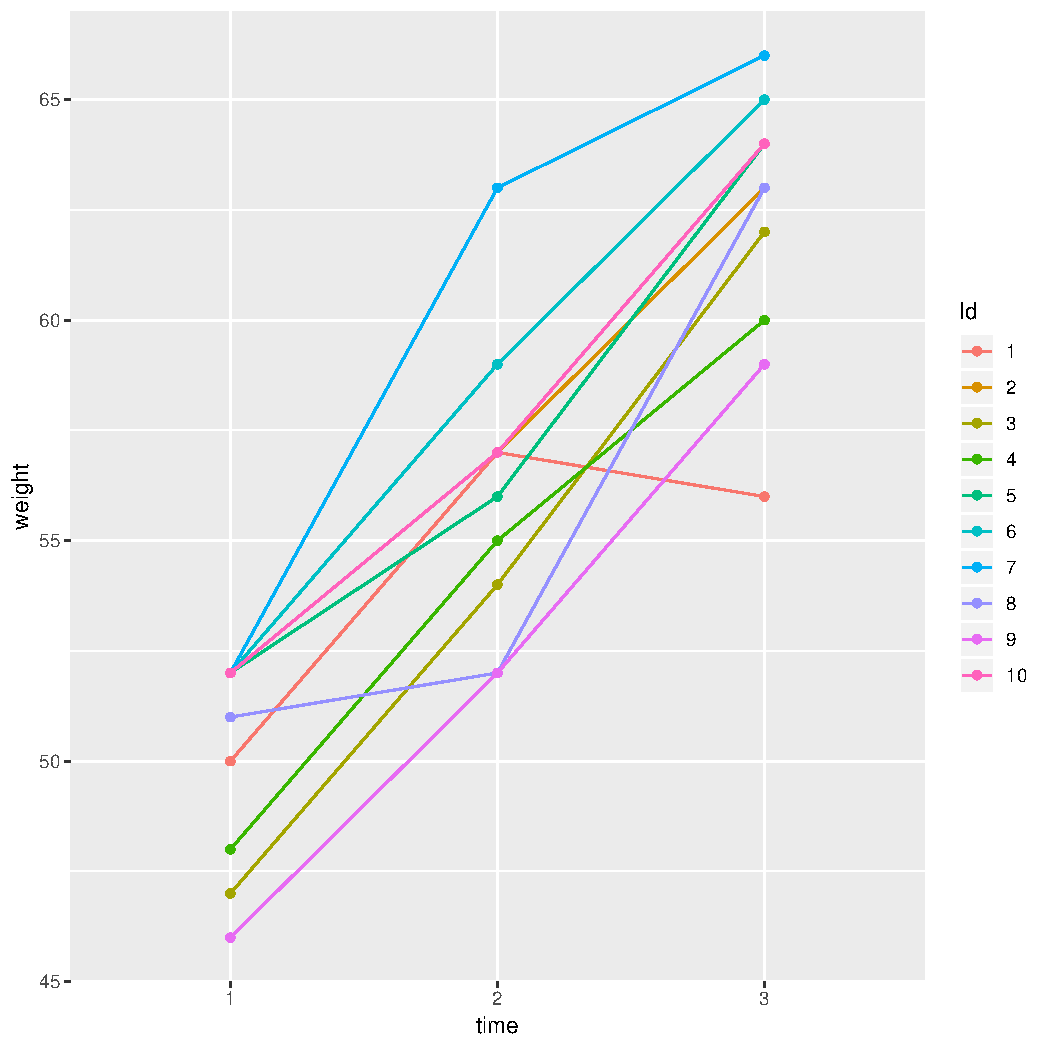
\includegraphics[width=0.65\textwidth]{./figures/fig-spaguetti1.pdf}
\end{center}


\clearpage

\item color by treatment group (first ten individuals)
\label{sec:org474488f}

\lstset{language=r,label= ,caption= ,captionpos=b,numbers=none}
\begin{lstlisting}
gg.spaguetti2 <- ggplot(dtL.data[Id %in% 1:10],
                        aes(x = time, y = weight, color = Treatment, group = Id))
gg.spaguetti2 <- gg.spaguetti2 + geom_line() + geom_point()
gg.spaguetti2
\end{lstlisting}

\begin{center}
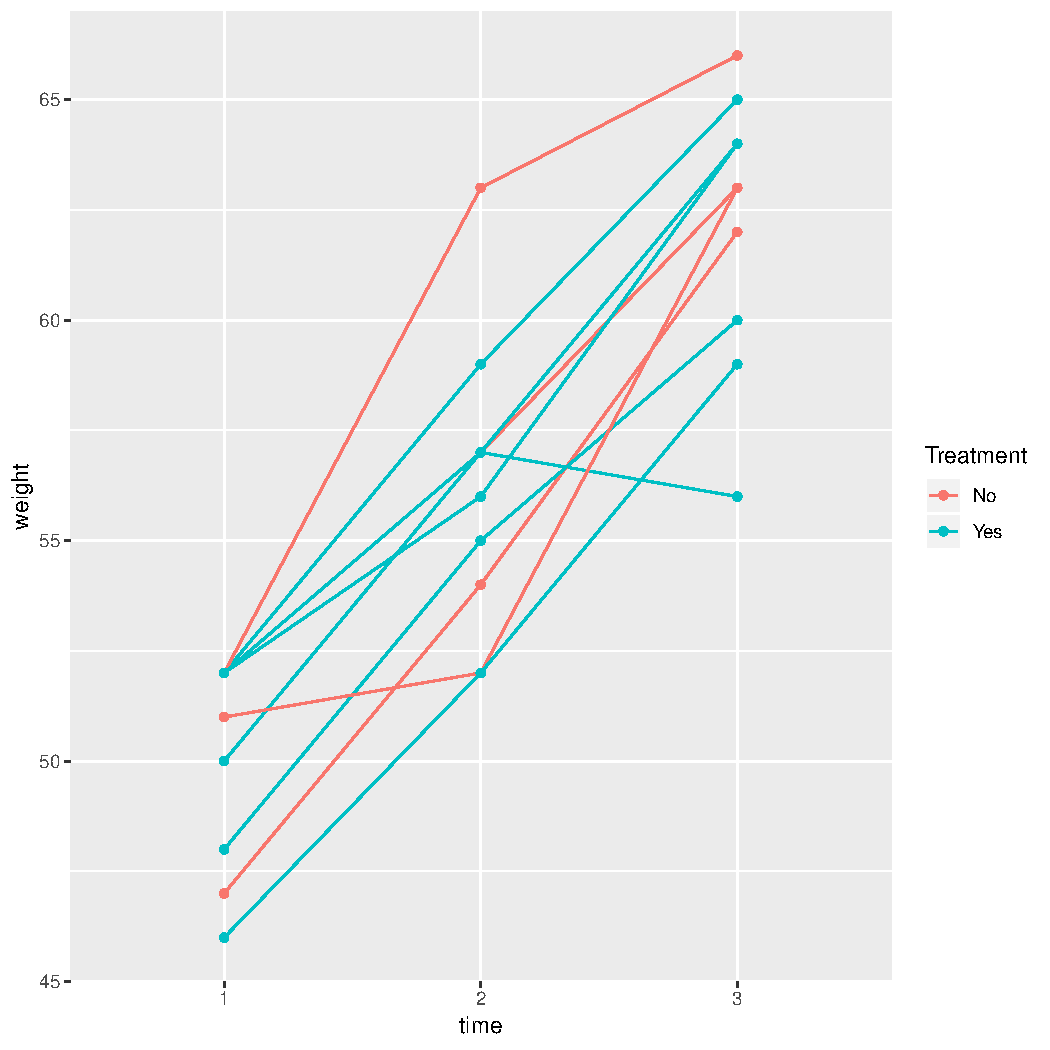
\includegraphics[width=0.8\textwidth]{./figures/fig-spaguetti2.pdf}
\end{center}


\clearpage 

\item pannel for each treatment group (first ten individuals)
\label{sec:orgd275c54}

\lstset{language=r,label= ,caption= ,captionpos=b,numbers=none}
\begin{lstlisting}
gg.spaguetti3 <- ggplot(dtL.data[Id %in% 1:10], 
                        aes(x = time, y = weight, color = Id, group = Id))
gg.spaguetti3 <- gg.spaguetti3 + geom_line() + geom_point()
gg.spaguetti3 <- gg.spaguetti3 + facet_wrap(~ Treatment, labeller = label_both) 
gg.spaguetti3
\end{lstlisting}

\begin{center}
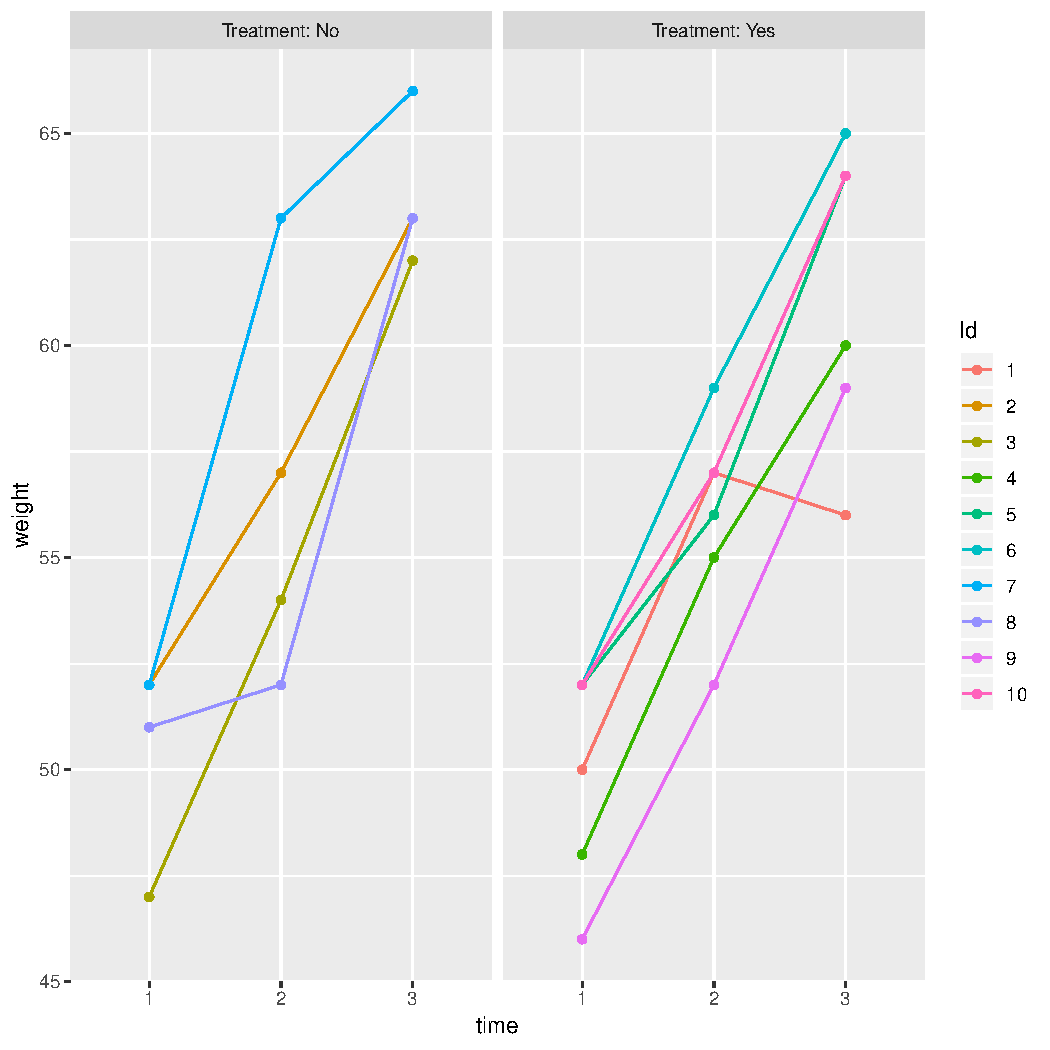
\includegraphics[width=0.8\textwidth]{./figures/fig-spaguetti3.pdf}
\end{center}


\clearpage

\item individual spaguetti plot (first ten individuals)
\label{sec:org3cb4a01}

\lstset{language=r,label= ,caption= ,captionpos=b,numbers=none}
\begin{lstlisting}
gg.spaguetti4 <- ggplot(dtL.data[Id %in% 1:10], 
                        aes(x = time, y = weight, color = Id, group = Id))
gg.spaguetti4 <- gg.spaguetti4 + geom_line() + geom_point()
gg.spaguetti4 <- gg.spaguetti4 + facet_wrap(~ Id, labeller = label_both) 
gg.spaguetti4
\end{lstlisting}

\begin{center}
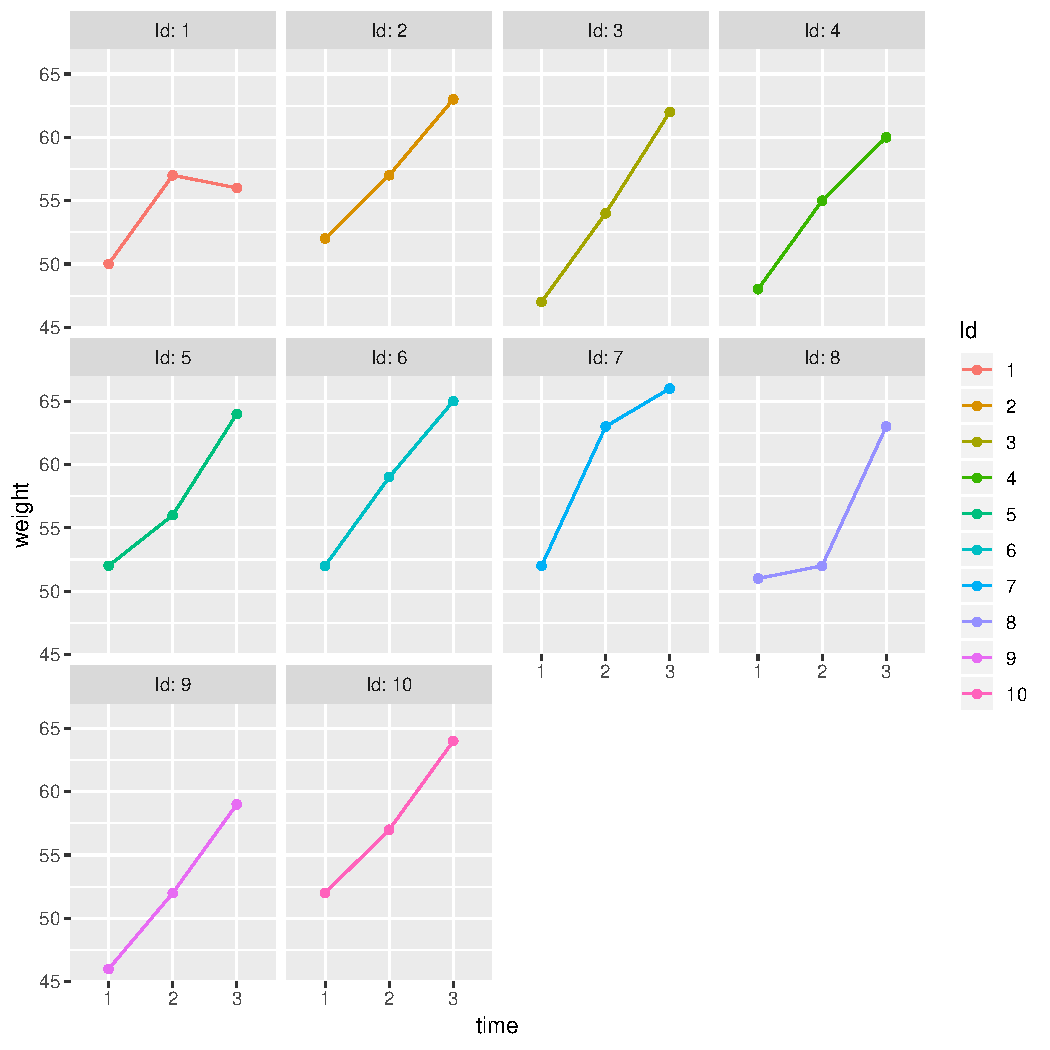
\includegraphics[width=0.8\textwidth]{./figures/fig-spaguetti4.pdf}
\end{center}

\clearpage
\end{enumerate}

\subsubsection{Display the mean over time}
\label{sec:org4a6de56}

\lstset{language=r,label= ,caption= ,captionpos=b,numbers=none}
\begin{lstlisting}
gg.mean <- ggplot(dtL.data[Id %in% 1:10], aes(x = time, y = weight))
gg.mean <- gg.mean + stat_summary(aes(group = Treatment, color = Treatment), 
                                  geom = "line", fun.y = mean, size = 2)
gg.mean <- gg.mean + stat_summary(aes(group = Treatment, color = Treatment), 
                                  geom = "point", fun.y = mean, size = 3)
\end{lstlisting}

\begin{center}
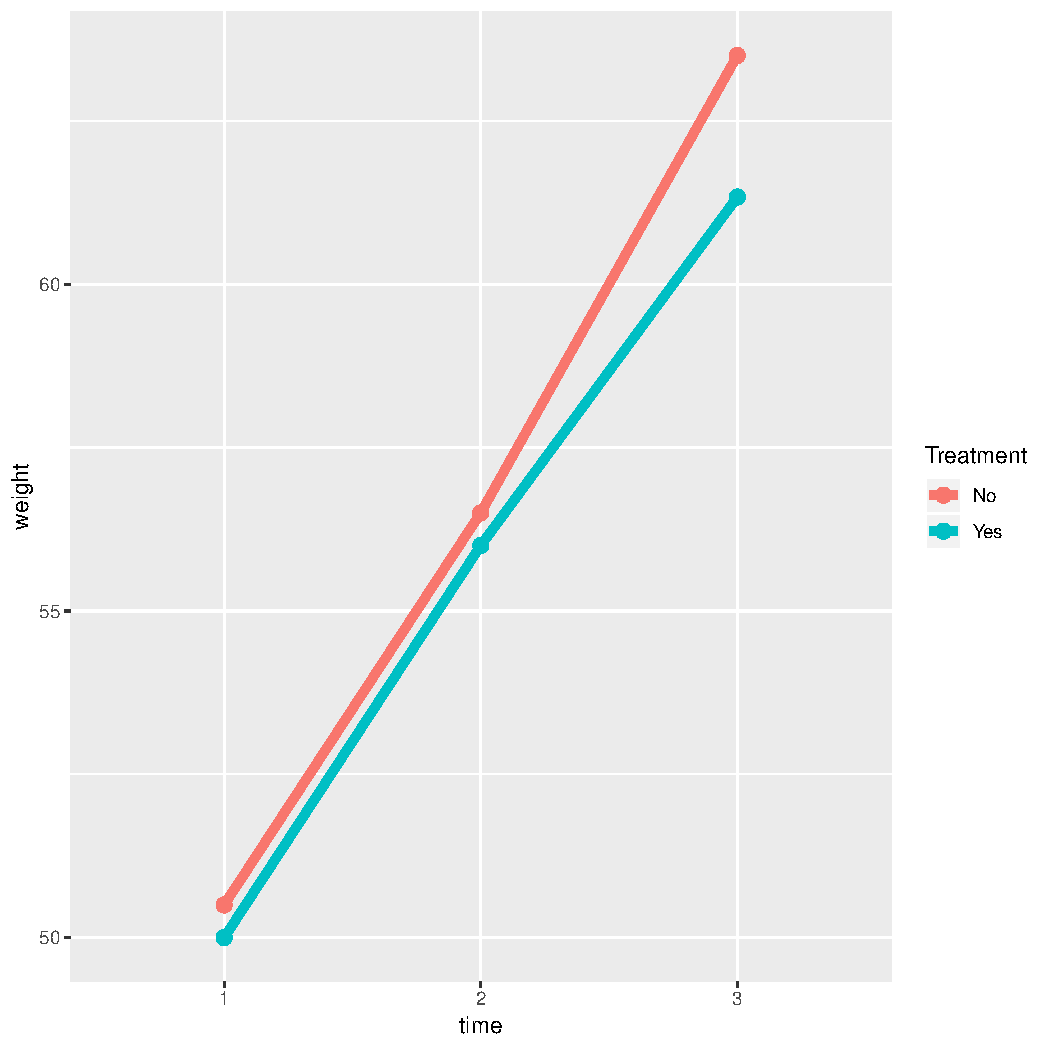
\includegraphics[width=.9\linewidth]{./figures/fig-meanTime.pdf}
\end{center}

\clearpage

\subsubsection{Boxplot + points (non-overlapping)}
\label{sec:orgb52eef7}

\lstset{language=r,label= ,caption= ,captionpos=b,numbers=none}
\begin{lstlisting}
gg.hist <- ggplot(dtL.data, aes(x = time, y = weight))
gg.hist <- gg.hist + geom_boxplot() 
gg.hist <- gg.hist + geom_dotplot(binaxis = "y", stackdir = "center", dotsize = 0.5)
gg.hist
\end{lstlisting}

\begin{verbatim}
`stat_bindot()` using `bins = 30`. Pick better value with `binwidth`.
\end{verbatim}



\begin{center}
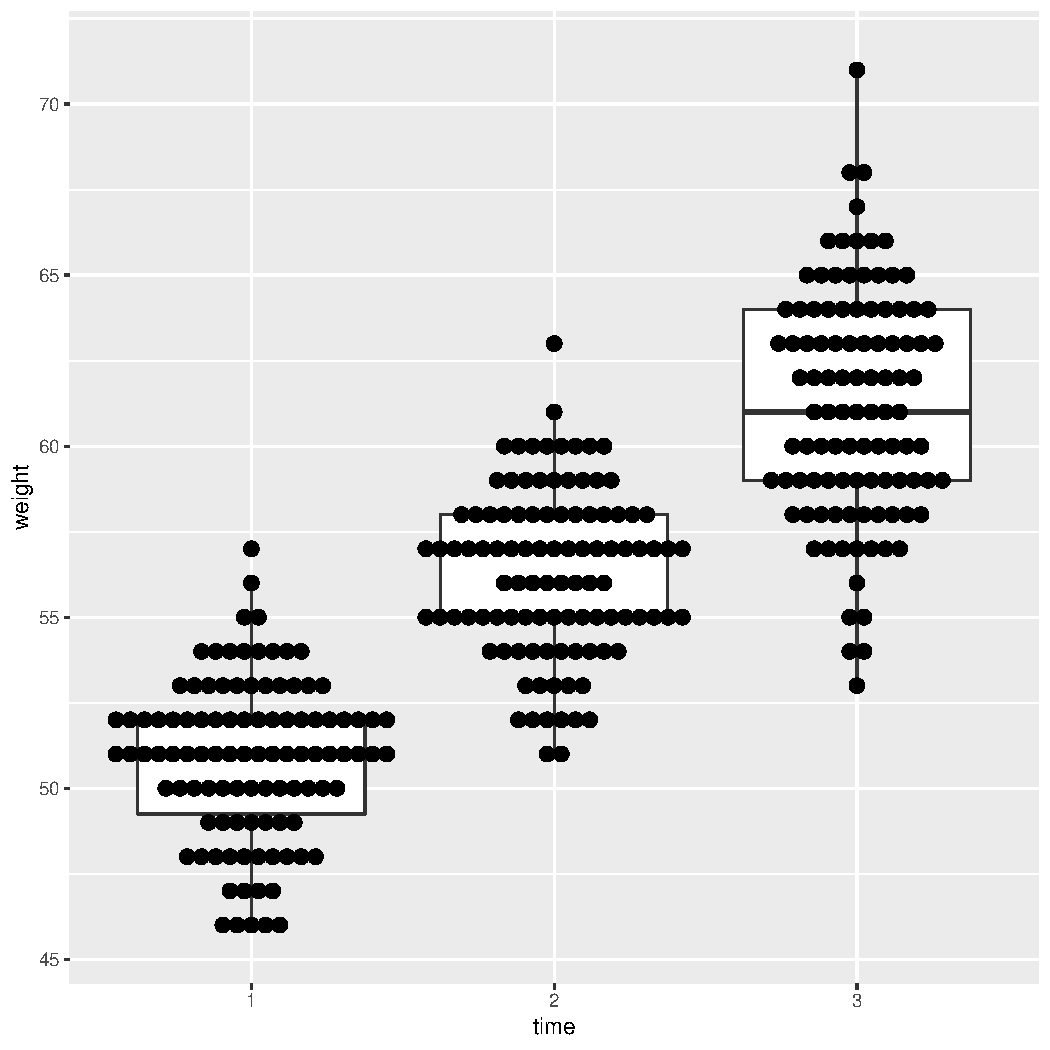
\includegraphics[width=.9\linewidth]{./figures/fig-hist.pdf}
\end{center}

\subsection{Diagnostic plots}
\label{sec:org9c01869}

Consider the linear model:
\lstset{language=r,label= ,caption= ,captionpos=b,numbers=none}
\begin{lstlisting}
e.lm <- lm(weight ~ Age + Treatment + size,
            data = dtL.data)
\end{lstlisting}

\subsubsection{Histogram of the residuals}
\label{sec:org36ac542}

Extract the residuals:
\lstset{language=r,label= ,caption= ,captionpos=b,numbers=none}
\begin{lstlisting}
epsilon <- residuals(e.lm, type = "response")
\end{lstlisting}

Display the histogram
\begin{center}
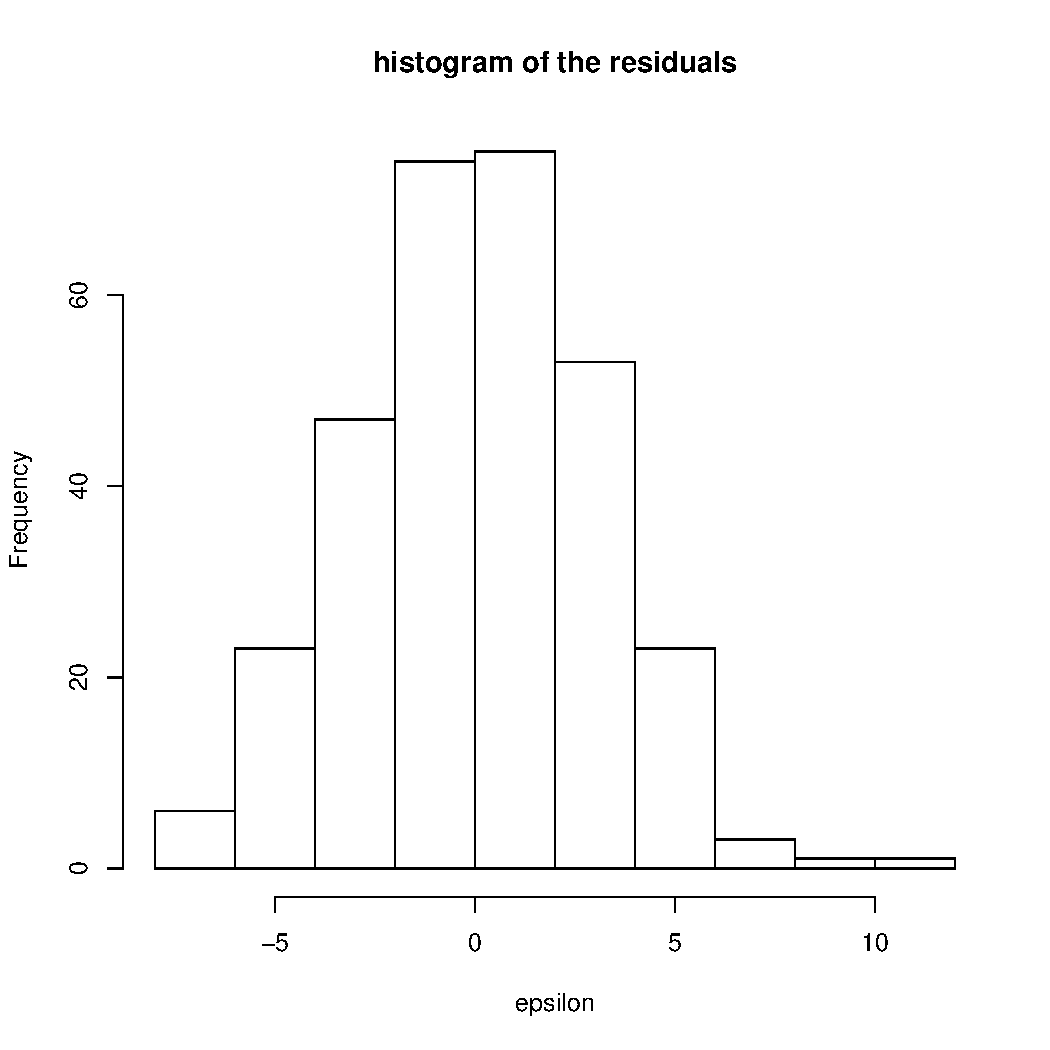
\includegraphics[width=.9\linewidth]{./figures/fig-hist-residuals.pdf}
\end{center}
\subsubsection{Forest plot}
\label{sec:orgb01f75f}
\lstset{language=r,label= ,caption= ,captionpos=b,numbers=none}
\begin{lstlisting}
## gg.forest <- ggplot(data=df.bcg, aes(x=label, y=Estimate, ymin=lower, ymax=upper))
## gg.forest <- gg.forest + geom_pointrange()
## gg.forest <- gg.forest + geom_hline(yintercept=1, lty=2) + coord_flip()
## gg.forest <- gg.forest + xlab("Label") + ylab("Mean (95% CI)") 
\end{lstlisting}

\subsection{Customize graphic}
\label{sec:org12440fe}

\subsubsection{Greek letter in facet}
\label{sec:org53e51ac}
\lstset{language=r,label= ,caption= ,captionpos=b,numbers=none}
\begin{lstlisting}
seqX <- 1:15
df <- rbind(data.frame(density = dpois(seqX,lambda = 1),
                       lambda = 1,
                       x = seqX),
            data.frame(density = dpois(seqX,lambda = 2),
                       lambda = 2,
                       x = seqX))

df$lambda <- factor(df$lambda, levels = c(1,2),
                    labels=c(expression(paste(lambda,"=1")),
                             expression(paste(lambda,"=2")))
                    )

library(ggplot2)
gg <- ggplot(df, aes(y=density,x=x)) + geom_bar(stat="identity")
gg + facet_wrap(~lambda, nrow = 1, labeller = label_parsed)

\end{lstlisting}

\subsubsection{Modify the legend of a discrete scale (with greek letters)}
\label{sec:orgec7b318}

\lstset{language=r,label= ,caption= ,captionpos=b,numbers=none}
\begin{lstlisting}
gg.mean2 <- gg.mean + scale_colour_manual(name = expression("Group"~(alpha*Omega)),
                                          labels = c("\u03b1\u2090","X\u1D30"),
                                          values = c("No" = "purple", 
                                                     "Yes" = "black"))
\end{lstlisting}

\begin{center}
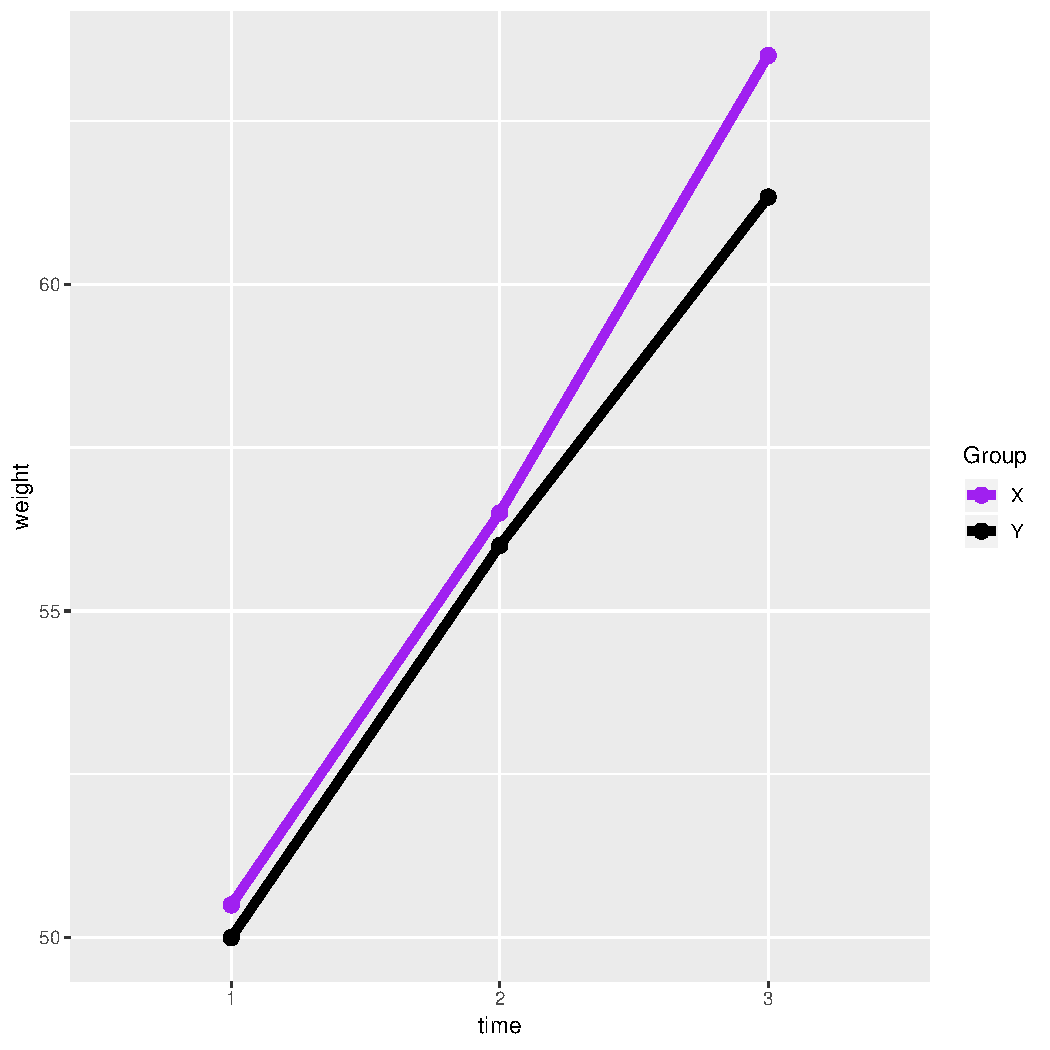
\includegraphics[width=0.8\textwidth]{./figures/fig-meanTime2.pdf}
\end{center}

See also:
\begin{itemize}
\item \url{https://en.wikipedia.org/wiki/List\_of\_Unicode\_characters}
\item \url{https://en.wikipedia.org/wiki/Unicode\_subscripts\_and\_superscripts}
\item \url{https://stackoverflow.com/questions/5293715/how-to-use-greek-symbols-in-ggplot2}
\end{itemize}

\clearpage
\subsubsection{Change the name of the legend}
\label{sec:org46e2017}
\lstset{language=r,label= ,caption= ,captionpos=b,numbers=none}
\begin{lstlisting}
gg.mean3 <- gg.mean2 + labs(colour="xyz")
\end{lstlisting}

\subsubsection{Increase the font size}
\label{sec:org3217dab}

All text:
\lstset{language=r,label= ,caption= ,captionpos=b,numbers=none}
\begin{lstlisting}
gg.mean3 <- gg.mean + theme(text = element_text(size=10))
\end{lstlisting}

\begin{center}
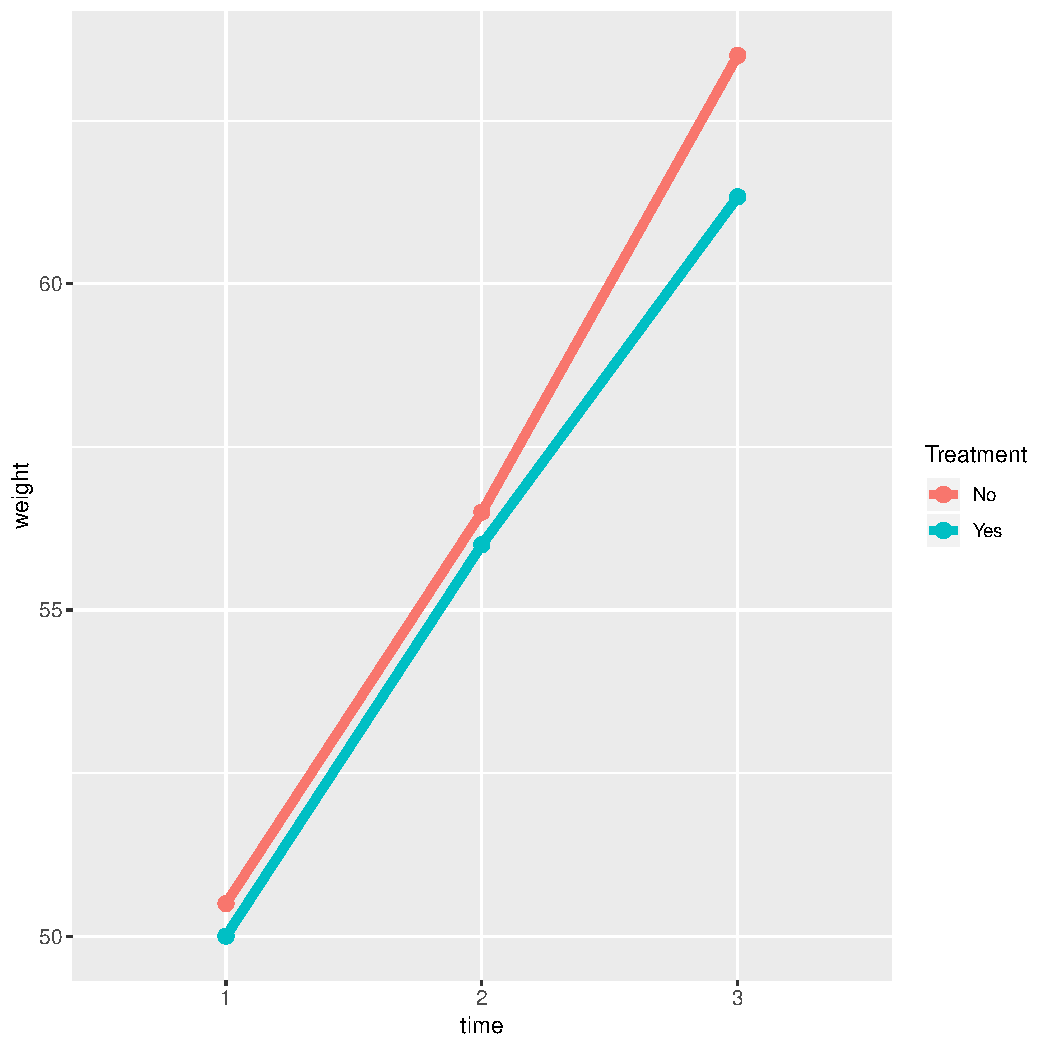
\includegraphics[width=0.8\textwidth]{./figures/fig-meanTime3.pdf}
\end{center}

Only x axis labels:
\lstset{language=r,label= ,caption= ,captionpos=b,numbers=none}
\begin{lstlisting}
gg.mean3 <- gg.mean + theme(axis.text = element_text(size=10))
\end{lstlisting}

Only axis title:
\lstset{language=r,label= ,caption= ,captionpos=b,numbers=none}
\begin{lstlisting}
gg.mean3 <- gg.mean + theme(axis.title = element_text(size=10))
\end{lstlisting}

\clearpage
\subsubsection{Increase size of the legend labels}
\label{sec:org804e143}
\lstset{language=r,label= ,caption= ,captionpos=b,numbers=none}
\begin{lstlisting}
    gg.mean + theme(text = element_text(size=15), 
                    axis.line = element_line(linewidth = 1.25),
                    axis.ticks = element_line(linewidth = 2),
                    axis.ticks.length=unit(.25, "cm"),
                    legend.key.size = unit(3,"line"))

    gg.mean + theme(axis.title = element_text(size=10), 
                    axis.line = element_line(linewidth = 1.25),
                    axis.ticks = element_line(linewidth = 2),
                    axis.ticks.length=unit(.25, "cm"),
                    legend.key.size = unit(3,"line"))
\end{lstlisting}

\subsubsection{Put the legend at the bottom}
\label{sec:orgee6a2da}
\lstset{language=r,label= ,caption= ,captionpos=b,numbers=none}
\begin{lstlisting}
gg.mean4 <- gg.mean + theme(legend.position="bottom",
                            legend.direction = "horizontal")
\end{lstlisting}

\begin{center}
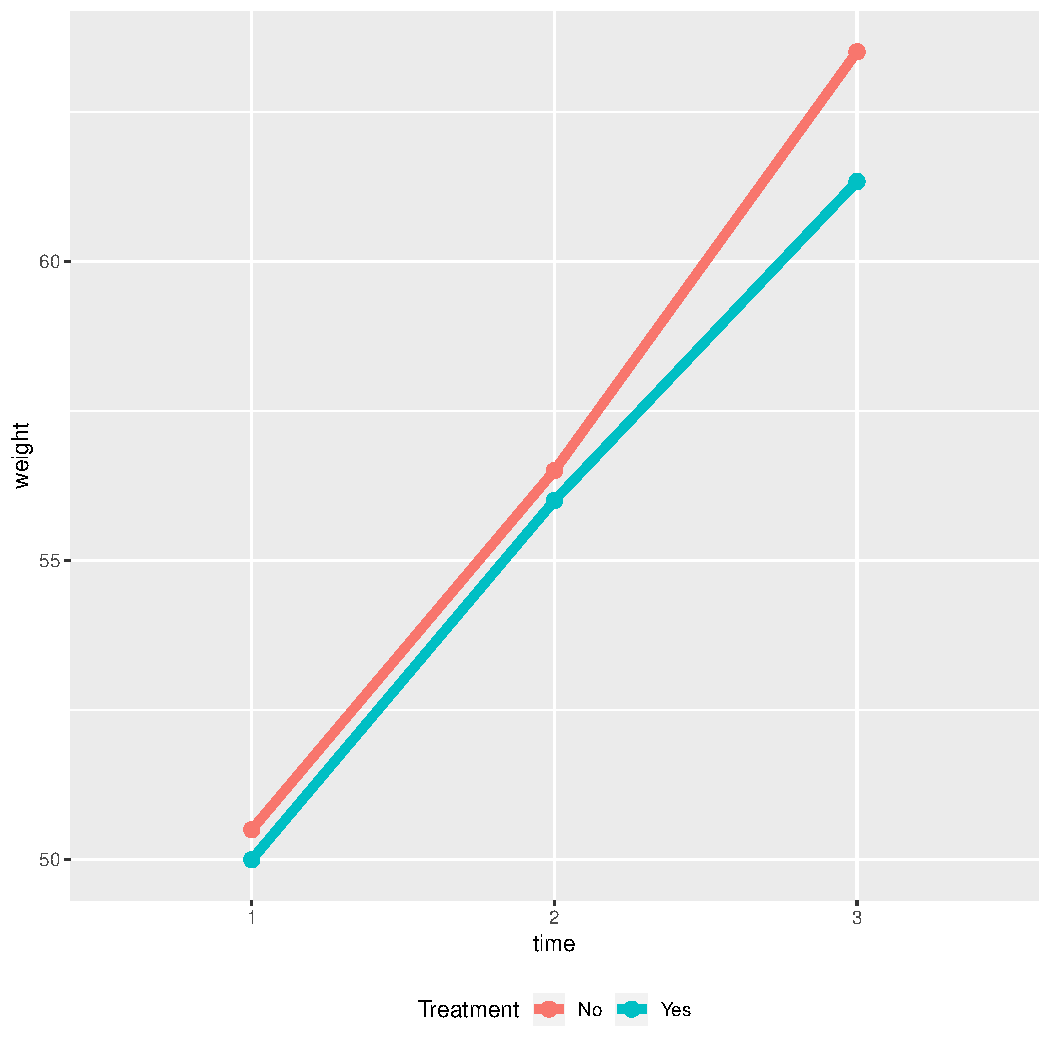
\includegraphics[trim={0 0 0 0},width=0.7\textwidth]{./figures/fig-meanTime4.pdf}
\end{center}
\clearpage
\subsubsection{Number of lines in the legend}
\label{sec:org0a39c06}
\lstset{language=r,label= ,caption= ,captionpos=b,numbers=none}
\begin{lstlisting}
gg.mean + guides(color = guide_legend(nrow = 2, byrow = TRUE))
\end{lstlisting}

\subsubsection{Default ggplot color palette}
\label{sec:orgb34cc80}

\lstset{language=r,label= ,caption= ,captionpos=b,numbers=none}
\begin{lstlisting}
gg_color_hue <- function(n) {
  hues = seq(15, 375, length = n + 1)
  hcl(h = hues, l = 65, c = 100)[1:n]
}
\end{lstlisting}

\subsubsection{Color blind palette}
\label{sec:org189d259}
\lstset{language=r,label= ,caption= ,captionpos=b,numbers=none}
\begin{lstlisting}
ggthemes::colorblind_pal()(8) ## also consider scale_color_colorblind
\end{lstlisting}

\begin{verbatim}
[1] "#000000" "#E69F00" "#56B4E9" "#009E73" "#F0E442" "#0072B2" "#D55E00" "#CC79A7"
\end{verbatim}

\subsubsection{Rotate x-axis labels}
\label{sec:orgc705da7}
\lstset{language=r,label= ,caption= ,captionpos=b,numbers=none}
\begin{lstlisting}
theme(axis.text.x = element_text(angle = 90, hjust = 1))
\end{lstlisting}

\subsubsection{Change tick mark labels}
\label{sec:orgf876cff}

\lstset{language=r,label= ,caption= ,captionpos=b,numbers=none}
\begin{lstlisting}
gg.mean5 <- gg.mean + scale_x_discrete(breaks=c("1","2","3"),
                                       labels=c("Dose 1", "Dose 2", "Dose 3"))
\end{lstlisting}

\begin{center}
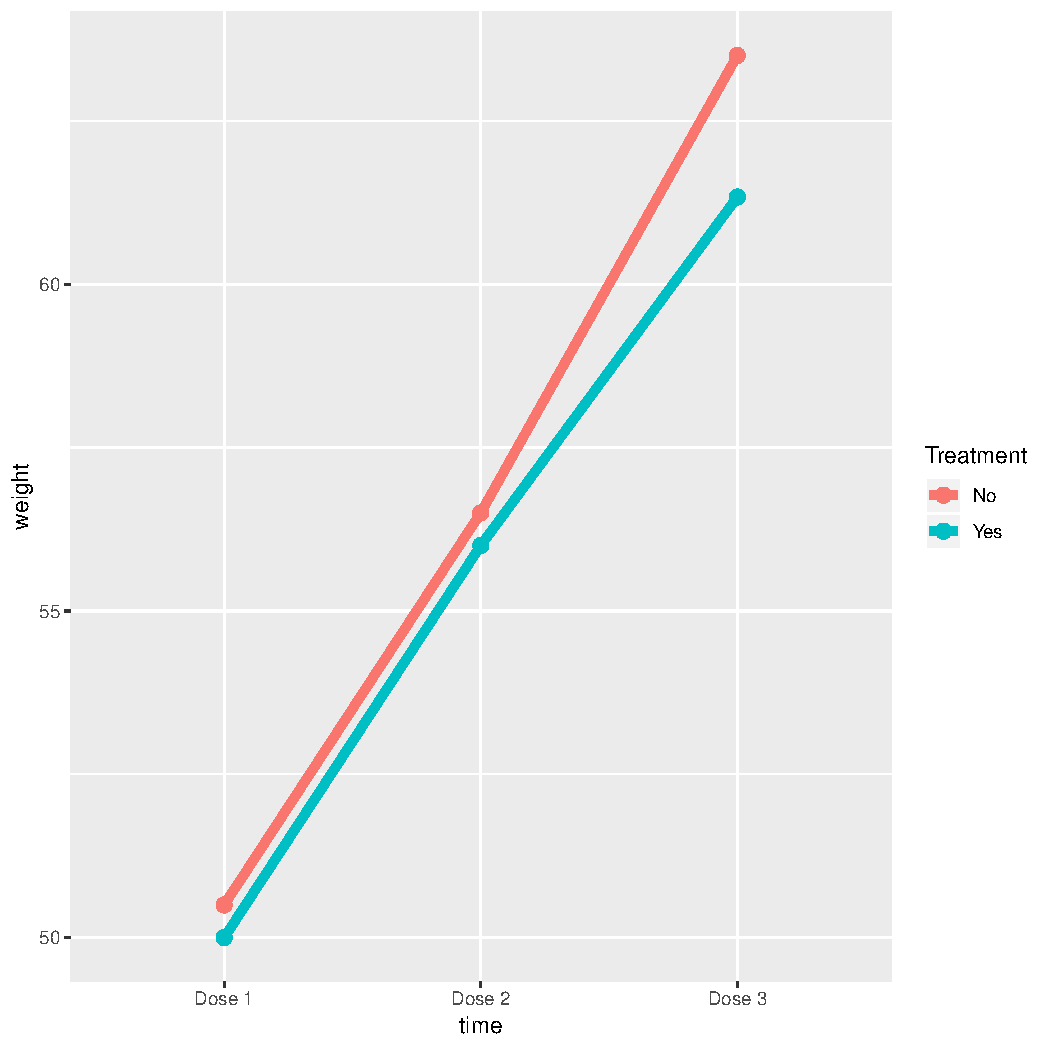
\includegraphics[width=.9\linewidth]{./figures/fig-meanTime5.pdf}
\end{center}

\clearpage

\subsubsection{Combine ggplots}
\label{sec:org90c681d}
(from \url{https://stackoverflow.com/questions/13649473/add-a-common-legend-for-combined-ggplots})

\lstset{language=r,label= ,caption= ,captionpos=b,numbers=none}
\begin{lstlisting}
library(ggpubr)

dsamp <- diamonds[sample(nrow(diamonds), 1000), ]
p1 <- qplot(carat, price, data = dsamp, colour = clarity)
p2 <- qplot(cut, price, data = dsamp, colour = clarity)
p3 <- qplot(color, price, data = dsamp, colour = clarity)
p4 <- qplot(depth, price, data = dsamp, colour = clarity) 

out <- ggarrange(p1, p2, p3, p4, ncol=2, nrow=2, common.legend = TRUE, legend="bottom")
\end{lstlisting}

\begin{center}
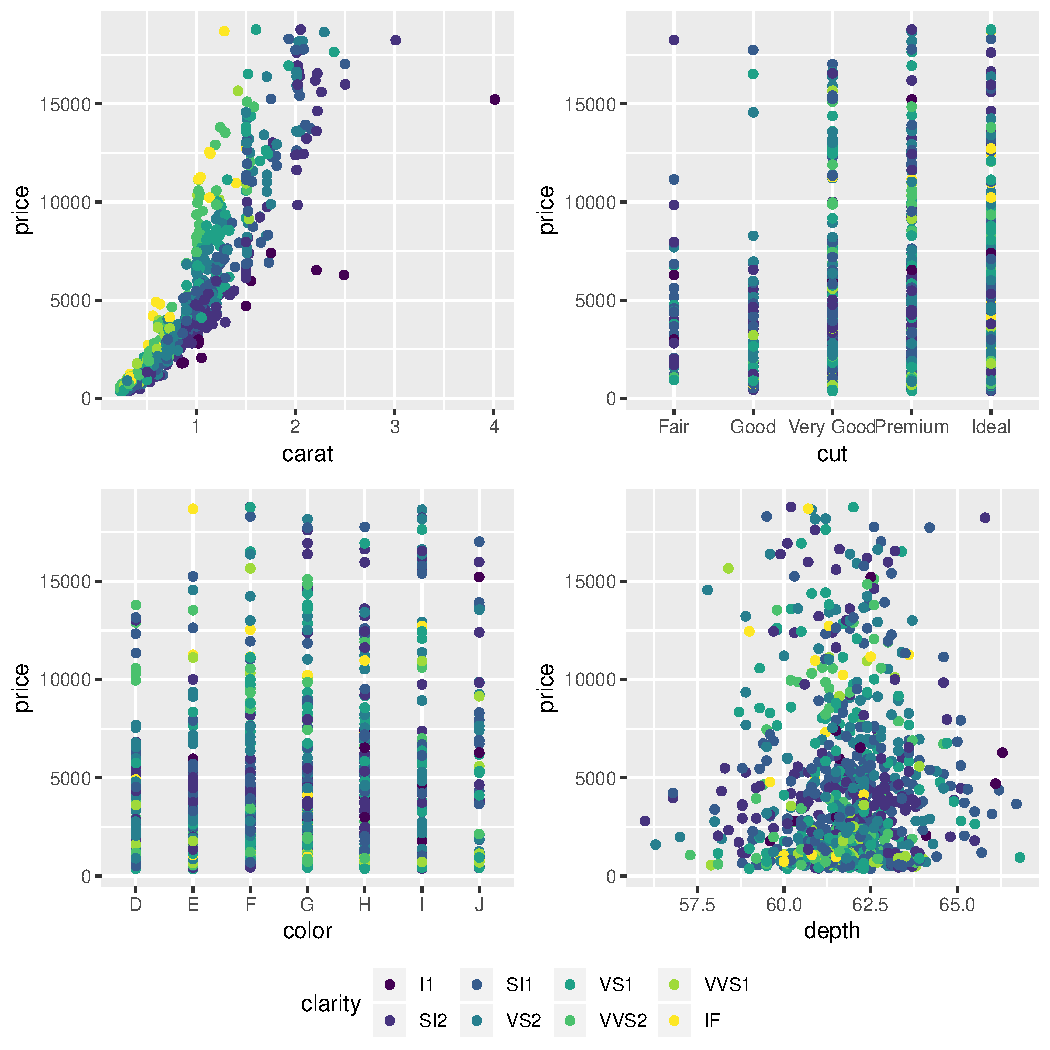
\includegraphics[width=.9\linewidth]{./figures/fig-combine.pdf}
\end{center}

\subsubsection{Symbols in facet names}
\label{sec:org5706b28}

\lstset{language=r,label= ,caption= ,captionpos=b,numbers=none}
\begin{lstlisting}
df <- data.frame(x = 1:5, y = rnorm(5), method = "df[num]+omega+sqrt(2)")
gg <- ggplot(df, aes(x,y)) + geom_point() + facet_grid(~method, labeller = label_parsed)
gg <- gg + theme(text = element_text(size=20))
gg
\end{lstlisting}

\begin{center}
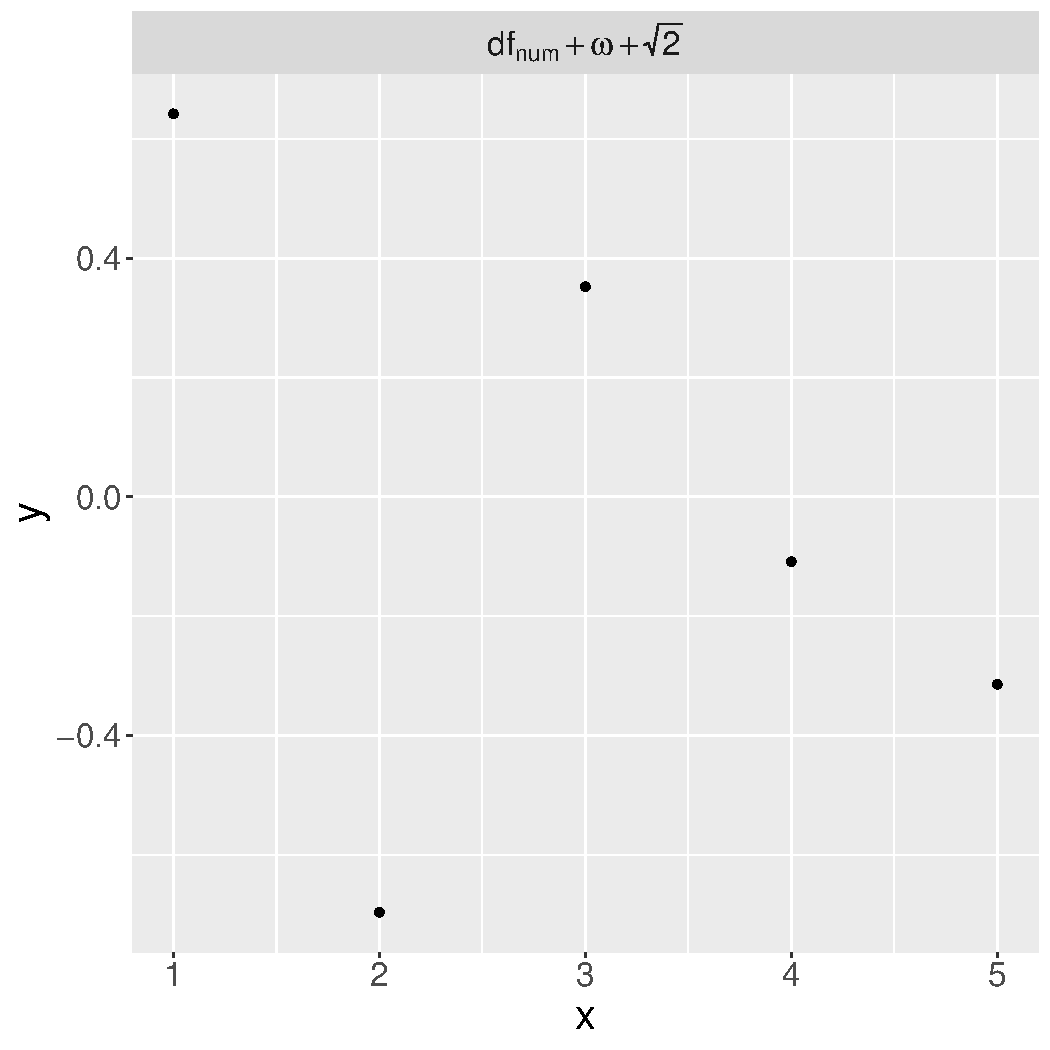
\includegraphics[trim={0 0 0 0},width=0.5\textwidth]{./figures/fig-symbolfacet.pdf}
\end{center}


\subsubsection{Extract labels of the x/y thicks}
\label{sec:org5fc3751}

\lstset{language=r,label= ,caption= ,captionpos=b,numbers=none}
\begin{lstlisting}
df <- rbind(data.frame(x = "a", y = rnorm(5)),
            data.frame(x = "b", y = rnorm(5)),
            data.frame(x = "c", y = rnorm(5)))

gg <- ggplot(df, aes(x,y)) + geom_boxplot()
ggplot_build(gg)$layout$panel_params[[1]]$x$get_labels()
\end{lstlisting}

\begin{verbatim}
[1] "a" "b" "c"
\end{verbatim}


\lstset{language=r,label= ,caption= ,captionpos=b,numbers=none}
\begin{lstlisting}
ggplot_build(gg)$layout$panel_params[[1]]$y$get_labels()
\end{lstlisting}

\begin{verbatim}
[1] "-2" "-1" "0"  "1"  NA
\end{verbatim}


\clearpage

\subsection{Path diagram}
\label{sec:orga8765d3}
Using lava:
\lstset{language=r,label= ,caption= ,captionpos=b,numbers=none}
\begin{lstlisting}
m <- lvm(Y~E+X1+X2+M,M~E,E~X2)
\end{lstlisting}

\lstset{language=r,label= ,caption= ,captionpos=b,numbers=none}
\begin{lstlisting}
plot(m, plot.engine="rgraphviz") 
\end{lstlisting}

Dynamic graph:
\lstset{language=r,label= ,caption= ,captionpos=b,numbers=none}
\begin{lstlisting}
plot(m, plot.engine="visnetwork")
\end{lstlisting}
\subsection{Lexis diagram}
\label{sec:org9504bce}

Simulate data
\lstset{language=r,label= ,caption= ,captionpos=b,numbers=none}
\begin{lstlisting}
library(riskRegression)
library(ggplot2)
library(data.table)

set.seed(10)
d <- sampleData(1000)
d[, id := as.character(1:.N)]
\end{lstlisting}

Reshape data
\lstset{language=r,label= ,caption= ,captionpos=b,numbers=none}
\begin{lstlisting}
d$Age <- d$X6
d$age.start <- d$Age
d$age.stop <- d$Age + d$time
d$start <- 0
d$stop <- d$time
dL <- rbind(d[,.(id = id, time = start, age = age.start, status = -1)],
            d[,.(id = id, time = stop, age = age.stop, status = event)])
dL[, event := factor(status, (-1):2, c("inclusion","censored","disease","death"))]
\end{lstlisting}
Display
\lstset{language=r,label= ,caption= ,captionpos=b,numbers=none}
\begin{lstlisting}
gg <- ggplot(dL, aes(x = time, y = age, group = id))
gg <- gg + geom_point(aes(color=event,shape=event)) 
gg <- gg + geom_line(alpha = 0.1) 
gg
\end{lstlisting}

\begin{center}
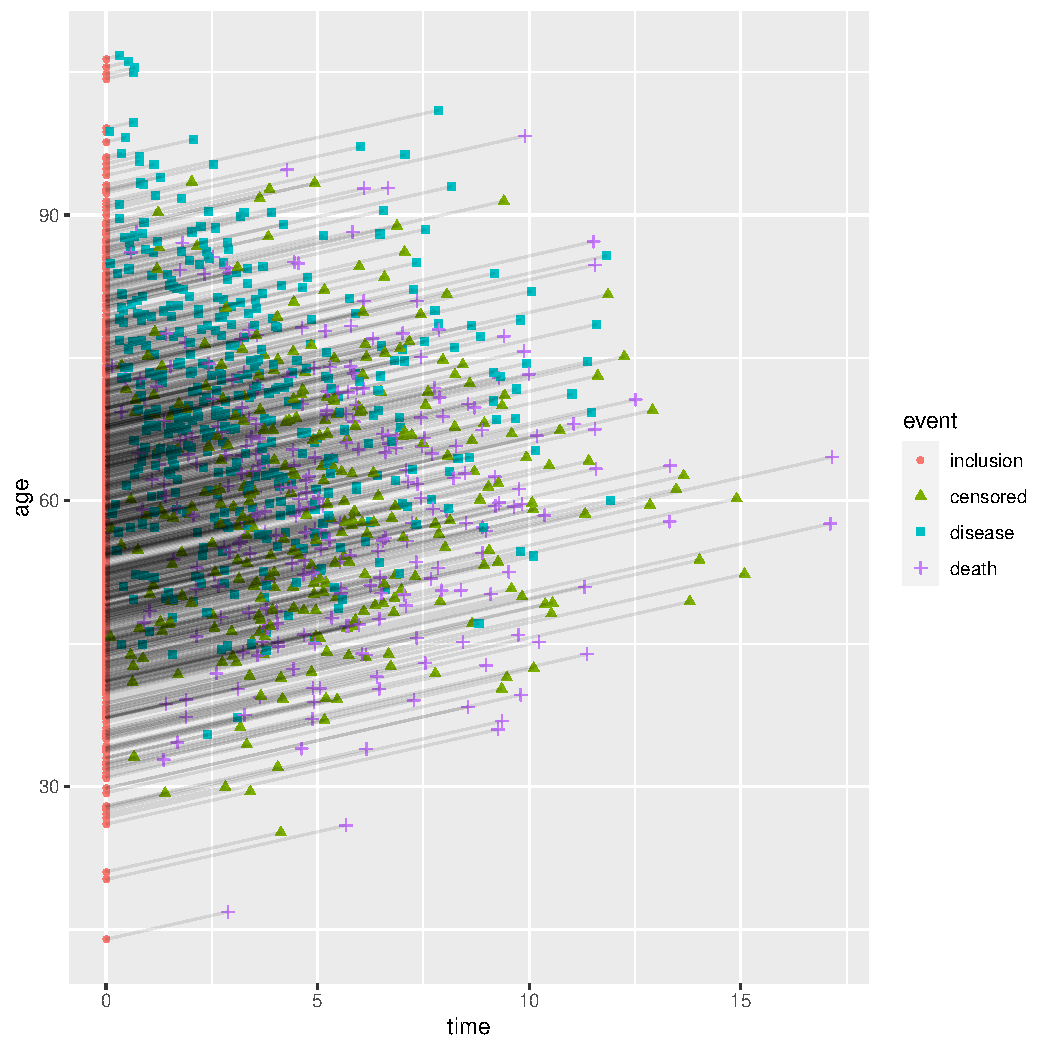
\includegraphics[width=1\textwidth]{./figures/fig-gg-lexis.pdf}
\end{center}

\subsection{Font}
\label{sec:org66c6812}
\subsubsection{Display available fonts}
\label{sec:orge4df73c}
\lstset{language=r,label= ,caption= ,captionpos=b,numbers=none}
\begin{lstlisting}
windowsFonts()
\end{lstlisting}

\begin{verbatim}
$serif
[1] "TT Times New Roman"

$sans
[1] "TT Arial"

$mono
[1] "TT Courier New"
\end{verbatim}


See also: \url{http://www.cookbook-r.com/Graphs/Fonts/}

\subsubsection{Add more fonts}
\label{sec:orgdc3c944}
\lstset{language=r,label= ,caption= ,captionpos=b,numbers=none}
\begin{lstlisting}
library(extrafont)
## font_import() ## only needed once
loadfonts(device = "win", quiet = TRUE)
head(windowsFonts())
\end{lstlisting}

\begin{verbatim}
$serif
[1] "TT Times New Roman"

$sans
[1] "TT Arial"

$mono
[1] "TT Courier New"

$`Agency FB`
[1] "Agency FB"

$Algerian
[1] "Algerian"

$`Arial Black`
[1] "Arial Black"
\end{verbatim}

\section{Modeling}
\label{sec:orgfc9cfed}
\subsection{Test proportions}
\label{sec:org1ef4a28}
\lstset{language=r,label= ,caption= ,captionpos=b,numbers=none}
\begin{lstlisting}
binom.exact(c(15,4), p = 0.5) ## 15 success, 4 failures
\end{lstlisting}

\begin{verbatim}

	Exact two-sided binomial test (central method)

data:  c(15, 4)
number of successes = 15, number of trials = 19, p-value = 0.01921
alternative hypothesis: true probability of success is not equal to 0.5
95 percent confidence interval:
 0.5443469 0.9394755
sample estimates:
probability of success 
             0.7894737
\end{verbatim}

\subsection{Compare proportions between groups}
\label{sec:orge5781a2}

Data:
\lstset{language=r,label= ,caption= ,captionpos=b,numbers=none}
\begin{lstlisting}
tab <- rbind(c(6,12),
             c(12,5))
colnames(tab) <- c("worse","better")
rownames(tab) <- c("Dalteparin","Placebo")
tab
\end{lstlisting}

\begin{verbatim}
           worse better
Dalteparin     6     12
Placebo       12      5
\end{verbatim}


\bigskip

\begin{itemize}
\item test conditional only on the sample sizes
\end{itemize}
\lstset{language=r,label= ,caption= ,captionpos=b,numbers=none}
\begin{lstlisting}
uncondExact2x2(x1 = tab[1,2],
               x2 = tab[2,2],
               n1 = sum(tab[1,]),
               n2 = sum(tab[2,]),
               conf.int = TRUE)
\end{lstlisting}

\begin{verbatim}

	Unconditional Exact Test on Difference in Proportions, method= FisherAdj, central

data:  x1/n1=(12/18) and x2/n2= (5/17)
proportion 1 = 0.66667, proportion 2 = 0.29412, p-value = 0.03488
alternative hypothesis: true p2-p1 is not equal to 0
95 percent confidence interval:
 -0.64591599 -0.02557945
sample estimates:
    p2-p1 
-0.372549
\end{verbatim}

Approximate test:
\lstset{language=r,label= ,caption= ,captionpos=b,numbers=none}
\begin{lstlisting}
binomMeld.test(x1 = tab[1,2],
               x2 = tab[2,2],
               n1 = sum(tab[1,]),
               n2 = sum(tab[2,])
               )
\end{lstlisting}

\begin{verbatim}

	melded binomial test for difference

data:  sample 1:(12/18), sample 2:(5/17)
proportion 1 = 0.66667, proportion 2 = 0.29412, p-value = 0.06059
alternative hypothesis: true difference is not equal to 0
95 percent confidence interval:
 -0.67110802  0.01375096
sample estimates:
difference (p2-p1) 
         -0.372549
\end{verbatim}

\lstset{language=r,label= ,caption= ,captionpos=b,numbers=none}
\begin{lstlisting}
binomMeld.test(x1 = tab[1,2],
               x2 = tab[2,2],
               n1 = sum(tab[1,]),
               n2 = sum(tab[2,]),
               parmtype = "ratio"
               )
\end{lstlisting}

\begin{verbatim}

	melded binomial test for ratio

data:  sample 1:(12/18), sample 2:(5/17)
proportion 1 = 0.66667, proportion 2 = 0.29412, p-value = 0.06059
alternative hypothesis: true ratio is not equal to 1
95 percent confidence interval:
 0.1465276 1.0287320
sample estimates:
ratio (p2/p1) 
    0.4411765
\end{verbatim}

\bigskip

\begin{itemize}
\item test conditional on the sample sizes and the number of events
\end{itemize}
\lstset{language=r,label= ,caption= ,captionpos=b,numbers=none}
\begin{lstlisting}
fisher.exact(tab)
\end{lstlisting}

\begin{verbatim}

	Two-sided Fisher's Exact Test (usual method using minimum likelihood)

data:  tab
p-value = 0.04371
alternative hypothesis: true odds ratio is not equal to 1
95 percent confidence interval:
 0.0435 0.9170
sample estimates:
odds ratio 
 0.2189021
\end{verbatim}

which is better than
\lstset{language=r,label= ,caption= ,captionpos=b,numbers=none}
\begin{lstlisting}
fisher.test(tab)
\end{lstlisting}

\begin{verbatim}

	Fisher's Exact Test for Count Data

data:  tab
p-value = 0.04371
alternative hypothesis: true odds ratio is not equal to 1
95 percent confidence interval:
 0.03888003 1.05649145
sample estimates:
odds ratio 
 0.2189021
\end{verbatim}
where confidence intervals and p-values are not consistent.

\bigskip

\begin{itemize}
\item Paired: (mc-nemar test)
\end{itemize}
\lstset{language=r,label= ,caption= ,captionpos=b,numbers=none}
\begin{lstlisting}
mcnemar.exact(tab) 
\end{lstlisting}

\begin{verbatim}

	Exact McNemar test (with central confidence intervals)

data:  tab
b = 12, c = 12, p-value = 1
alternative hypothesis: true odds ratio is not equal to 1
95 percent confidence interval:
 0.4109184 2.4335733
sample estimates:
odds ratio 
         1
\end{verbatim}

\subsection{Estimate Mann Whitney parameter}
\label{sec:orge50702b}

Remove ties:
\lstset{language=r,label= ,caption= ,captionpos=b,numbers=none}
\begin{lstlisting}
set.seed(10)
sleep$Y <- sleep$extra + rnorm(NROW(sleep), sd = 0.1)
\end{lstlisting}

Original p-value:
\lstset{language=r,label= ,caption= ,captionpos=b,numbers=none}
\begin{lstlisting}
suppressWarnings(wilcox.test(Y ~ group, data = sleep, exact = FALSE)$p.value)
\end{lstlisting}

\begin{verbatim}
[1] 0.03763531
\end{verbatim}


Mann-Whitney parameter (method 1)
\lstset{language=r,label= ,caption= ,captionpos=b,numbers=none}
\begin{lstlisting}
library(asht)
wmwTest(Y ~ group, data = sleep, method = "asymptotic")
\end{lstlisting}

\begin{verbatim}

	Wilcoxon-Mann-Whitney test with continuity correction (confidence interval requires proportional odds assumption,
	but test does not)

data:  Y by group
Mann-Whitney estimate = 0.78, tie factor = 1, p-value = 0.03764
alternative hypothesis: two distributions are not equal
95 percent confidence interval:
 0.5158768 0.9172200
sample estimates:
Mann-Whitney estimate 
                 0.78
\end{verbatim}

Mann-Whitney parameter (method 2)
\lstset{language=r,label= ,caption= ,captionpos=b,numbers=none}
\begin{lstlisting}
library(BuyseTest)
BuyseTest.options(order.Hprojection=2)
e.BT <- BuyseTest(group ~ cont(Y), data = sleep, 
                  method.inference = "u-statistic")
confint(e.BT, statistic = "favorable")
\end{lstlisting}

\begin{verbatim}
        estimate     se  lower.ci  upper.ci    p.value
Y_1e-12     0.78 0.1049 0.5168762 0.9215649 0.03841179
attr(,"n.resampling")
Y_1e-12 
     NA
\end{verbatim}

\subsection{Permutation t-test: 2 group comparison}
\label{sec:orgbd3958b}

Data:
\lstset{language=r,label= ,caption= ,captionpos=b,numbers=none}
\begin{lstlisting}
set.seed(10)
X <- rlnorm(10, meanlog = 2, sdlog = 0.5)
Y <- rlnorm(10, meanlog = 1.8, sdlog = 0.5)
\end{lstlisting}

Approximation based on asymptotic result:
\lstset{language=r,label= ,caption= ,captionpos=b,numbers=none}
\begin{lstlisting}
permTS(x = X, y = Y, method = "pclt")
\end{lstlisting}

\begin{verbatim}

	Permutation Test using Asymptotic Approximation

data:  X and Y
Z = -1.5476, p-value = 0.1217
alternative hypothesis: true mean X - mean Y is not equal to 0
sample estimates:
mean X - mean Y 
      -1.533514
\end{verbatim}


Approximation based on simulations:
\lstset{language=r,label= ,caption= ,captionpos=b,numbers=none}
\begin{lstlisting}
permTS(x = X, y = Y, method = "exact.mc")
\end{lstlisting}

\begin{verbatim}

	Exact Permutation Test Estimated by Monte Carlo

data:  X and Y
p-value = 0.112
alternative hypothesis: true mean X - mean Y is not equal to 0
sample estimates:
mean X - mean Y 
      -1.533514 

p-value estimated from 999 Monte Carlo replications
99 percent confidence interval on p-value:
 0.07625212 0.15272627
\end{verbatim}

Exact:
\lstset{language=r,label= ,caption= ,captionpos=b,numbers=none}
\begin{lstlisting}
permTS(x = X, y = Y, method = "exact.ce")
\end{lstlisting}

\begin{verbatim}

	Exact Permutation Test (complete enumeration)

data:  X and Y
p-value = 0.1238
alternative hypothesis: true mean X - mean Y is not equal to 0
sample estimates:
mean X - mean Y 
      -1.533514
\end{verbatim}

\subsection{Permutation t-test: multiple group comparison}
\label{sec:org48c5a18}
Data:
\lstset{language=r,label= ,caption= ,captionpos=b,numbers=none}
\begin{lstlisting}
set.seed(10)
X <- rlnorm(10, meanlog = 2, sdlog = 0.5)
Y <- rlnorm(10, meanlog = 1.8, sdlog = 0.5)
Z <- rlnorm(10, meanlog = 1.5, sdlog = 0.5)
df <- rbind(data.frame(value = X, group = "X"),
            data.frame(value = Y, group = "Y"),
            data.frame(value = Z, group = "Z"))
\end{lstlisting}

NOT VALIDATED!!! 
\lstset{language=r,label= ,caption= ,captionpos=b,numbers=none}
\begin{lstlisting}
library("permuco")
lmperm(value ~ group, data = df, np = 1e4)
\end{lstlisting}

\begin{verbatim}
Table of marginal t-test of the betas
Permutation test using freedman_lane to handle nuisance variables and 10000 permutations.
            Estimate Std. Error t value parametric Pr(>|t|) permutation Pr(<t) permutation Pr(>t) permutation Pr(>|t|)
(Intercept)    6.091     0.5755  10.584           4.142e-11                                                           
groupY         1.534     0.8139   1.884           7.035e-02             0.9631             0.0370               0.0716
groupZ        -3.095     0.8139  -3.803           7.440e-04             0.0005             0.9996               0.0009
\end{verbatim}

\subsection{Testing median}
\label{sec:orga69fad6}

Data:
\lstset{language=r,label= ,caption= ,captionpos=b,numbers=none}
\begin{lstlisting}
set.seed(10)
X <- rlnorm(100, meanlog = 2, sdlog = 0.5) - 6.5
\end{lstlisting}

Median test
\lstset{language=r,label= ,caption= ,captionpos=b,numbers=none}
\begin{lstlisting}
quantileTest(X)
\end{lstlisting}

\begin{verbatim}

	Exact Test/Confidence Interval for Median

data:  X
quantile for prob = 0.5, pAG = 0.18410, pAL = 0.86437, pc = 0.36820, p-value = 0.3682
alternative hypothesis: true median is not equal to 0
95 percent confidence interval:
 -0.3701565  1.4997902
sample estimates:
   median 
0.2082777
\end{verbatim}

\lstset{language=r,label= ,caption= ,captionpos=b,numbers=none}
\begin{lstlisting}
df <- data.frame(value=X)
e <- rq(value~1, tau = 0.5, data = df)
summary(e, se = "nid")
\end{lstlisting}

\begin{verbatim}
Warning message:
In rq.fit.br(x, y, tau = tau, ...) : Solution may be nonunique

Call: rq(formula = value ~ 1, tau = 0.5, data = df)

tau: [1] 0.5

Coefficients:
            Value   Std. Error t value Pr(>|t|)
(Intercept) 0.20213 0.49381    0.40932 0.68319
\end{verbatim}

Other quantiles
\lstset{language=r,label= ,caption= ,captionpos=b,numbers=none}
\begin{lstlisting}
e2 <- rq(value~1, tau = c(0.25,0.5,0.75), data = df)
summary(e2, se = "nid")
\end{lstlisting}

\begin{verbatim}
Warning messages:
1: In rq.fit.br(x, y, tau = tau, ...) : Solution may be nonunique
2: In rq.fit.br(x, y, tau = tau, ...) : Solution may be nonunique
3: In rq.fit.br(x, y, tau = tau, ...) : Solution may be nonunique

Call: rq(formula = value ~ 1, tau = c(0.25, 0.5, 0.75), data = df)

tau: [1] 0.25

Coefficients:
            Value    Std. Error t value  Pr(>|t|)
(Intercept) -1.61744  0.37283   -4.33828  0.00003

Call: rq(formula = value ~ 1, tau = c(0.25, 0.5, 0.75), data = df)

tau: [1] 0.5

Coefficients:
            Value   Std. Error t value Pr(>|t|)
(Intercept) 0.20213 0.49381    0.40932 0.68319 

Call: rq(formula = value ~ 1, tau = c(0.25, 0.5, 0.75), data = df)

tau: [1] 0.75

Coefficients:
            Value   Std. Error t value Pr(>|t|)
(Intercept) 3.43848 0.68607    5.01186 0.00000
\end{verbatim}

\subsection{Testing linear hypotheses}
\label{sec:orgd7f75db}

Consider the linear model:
\lstset{language=r,label= ,caption= ,captionpos=b,numbers=none}
\begin{lstlisting}
e.lm <- lm(weight ~ Age + Treatment + size,
            data = dtL.data)
summary(e.lm)$coef
\end{lstlisting}

\begin{verbatim}
                Estimate Std. Error    t value     Pr(>|t|)
(Intercept)  13.11292977 5.84498969  2.2434479 2.559263e-02
Age          -0.05479836 0.13849481 -0.3956709 6.926272e-01
TreatmentYes -0.65247721 0.36126020 -1.8061143 7.189597e-02
size          0.81718969 0.03513376 23.2593869 2.743182e-69
\end{verbatim}


To test linear hypotheses we first need to define them using a contrast matrix:
\lstset{language=r,label= ,caption= ,captionpos=b,numbers=none}
\begin{lstlisting}
name.coef <- names(coef(e.lm))
n.coef <- length(name.coef)

C <- matrix(0,nrow = 3, ncol = n.coef, 
            dimnames = list (c("Age","2 Treatment","All"), name.coef))
C["Age","Age"] <- 1
C["2 Treatment","TreatmentYes"] <- 2
C["All",-1] <- 1
C
\end{lstlisting}

\begin{verbatim}
            (Intercept) Age TreatmentYes size
Age                   0   1            0    0
2 Treatment           0   0            2    0
All                   0   1            1    1
\end{verbatim}

\subsubsection{Separate Wald tests of linear hypotheses}
\label{sec:org69c2df7}

No adjustment for multiple comparison:
\lstset{language=r,label= ,caption= ,captionpos=b,numbers=none}
\begin{lstlisting}
summary(glht(e.lm, linfct = C), test = univariate())
\end{lstlisting}

\begin{verbatim}

	 Simultaneous Tests for General Linear Hypotheses

Fit: lm(formula = weight ~ Age + Treatment + size, data = dtL.data)

Linear Hypotheses:
                 Estimate Std. Error t value Pr(>|t|)  
Age == 0          -0.0548     0.1385  -0.396   0.6926  
2 Treatment == 0  -1.3050     0.7225  -1.806   0.0719 .
All == 0           0.1099     0.3513   0.313   0.7546  
---
Signif. codes:  0 '***' 0.001 '**' 0.01 '*' 0.05 '.' 0.1 ' ' 1
(Univariate p values reported)
\end{verbatim}

Adjustment using bonferroni:
\lstset{language=r,label= ,caption= ,captionpos=b,numbers=none}
\begin{lstlisting}
summary(glht(e.lm, linfct = C), test = adjusted("bonferroni"))
\end{lstlisting}

\begin{verbatim}

	 Simultaneous Tests for General Linear Hypotheses

Fit: lm(formula = weight ~ Age + Treatment + size, data = dtL.data)

Linear Hypotheses:
                 Estimate Std. Error t value Pr(>|t|)
Age == 0          -0.0548     0.1385  -0.396    1.000
2 Treatment == 0  -1.3050     0.7225  -1.806    0.216
All == 0           0.1099     0.3513   0.313    1.000
(Adjusted p values reported -- bonferroni method)
\end{verbatim}

Adjustment using the max statistic:
\lstset{language=r,label= ,caption= ,captionpos=b,numbers=none}
\begin{lstlisting}
summary(glht(e.lm, linfct = C), test = adjusted("single-step"))
\end{lstlisting}

\begin{verbatim}

	 Simultaneous Tests for General Linear Hypotheses

Fit: lm(formula = weight ~ Age + Treatment + size, data = dtL.data)

Linear Hypotheses:
                 Estimate Std. Error t value Pr(>|t|)
Age == 0          -0.0548     0.1385  -0.396    0.916
2 Treatment == 0  -1.3050     0.7225  -1.806    0.157
All == 0           0.1099     0.3513   0.313    0.948
(Adjusted p values reported -- single-step method)
\end{verbatim}

Alternative syntax (without contrast matrix):
\lstset{language=r,label= ,caption= ,captionpos=b,numbers=none}
\begin{lstlisting}
summary(glht(e.lm, 
             linfct = c("Age = 0",
                        "2*TreatmentYes = 0",
                        "Age + TreatmentYes + size = 0")), 
        test = adjusted("single-step"))
\end{lstlisting}

\begin{verbatim}

	 Simultaneous Tests for General Linear Hypotheses

Fit: lm(formula = weight ~ Age + Treatment + size, data = dtL.data)

Linear Hypotheses:
                               Estimate Std. Error t value Pr(>|t|)
Age == 0                        -0.0548     0.1385  -0.396    0.916
2 * TreatmentYes == 0           -1.3050     0.7225  -1.806    0.157
Age + TreatmentYes + size == 0   0.1099     0.3513   0.313    0.948
(Adjusted p values reported -- single-step method)
\end{verbatim}

\subsubsection{Confidence intervals associated with linear hypotheses}
\label{sec:org5c356ec}

With no adjustment for multiplicity:
\lstset{language=r,label= ,caption= ,captionpos=b,numbers=none}
\begin{lstlisting}
confint(glht(e.lm, linfct = C), calpha = univariate_calpha())
\end{lstlisting}

\begin{verbatim}

	 Simultaneous Confidence Intervals

Fit: lm(formula = weight ~ Age + Treatment + size, data = dtL.data)

Quantile = 1.9679
95% confidence level
 

Linear Hypotheses:
                 Estimate lwr     upr    
Age == 0         -0.0548  -0.3273  0.2177
2 Treatment == 0 -1.3050  -2.7268  0.1169
All == 0          0.1099  -0.5815  0.8013
\end{verbatim}

With adjustment for multiplicity:
\lstset{language=r,label= ,caption= ,captionpos=b,numbers=none}
\begin{lstlisting}
confint(glht(e.lm, linfct = C), calpha = adjusted_calpha())
\end{lstlisting}

\begin{verbatim}

	 Simultaneous Confidence Intervals

Fit: lm(formula = weight ~ Age + Treatment + size, data = dtL.data)

Quantile = 2.314
95% family-wise confidence level
 

Linear Hypotheses:
                 Estimate lwr     upr    
Age == 0         -0.0548  -0.3753  0.2657
2 Treatment == 0 -1.3050  -2.9769  0.3670
All == 0          0.1099  -0.7031  0.9229
\end{verbatim}

\subsubsection{Joint test of linear hypotheses}
\label{sec:orgb6382f0}

One can use the \texttt{Ftest()} or \texttt{Chisqtest()} to obtain a joint test:
\lstset{language=r,label= ,caption= ,captionpos=b,numbers=none}
\begin{lstlisting}
summary(glht(e.lm, 
             linfct = c("Age = 0",
                        "2*TreatmentYes = 0",
                        "Age + TreatmentYes + size = 0")), 
        test = Ftest())
\end{lstlisting}

\begin{verbatim}

	 General Linear Hypotheses

Linear Hypotheses:
                               Estimate
Age == 0                        -0.0548
2 * TreatmentYes == 0           -1.3050
Age + TreatmentYes + size == 0   0.1099

Global Test:
      F DF1 DF2    Pr(>F)
1 181.2   3 302 3.349e-67
\end{verbatim}

The same can be obtained using the \texttt{linearHypothesis} method from the \texttt{car} package:
\lstset{language=r,label= ,caption= ,captionpos=b,numbers=none}
\begin{lstlisting}
linearHypothesis(e.lm, hypothesis.matrix = C, rhs = c(0,0,0))
\end{lstlisting}

\begin{verbatim}
Linear hypothesis test

Hypothesis:
Age = 0
2 TreatmentYes = 0
Age  + TreatmentYes  + size = 0

Model 1: restricted model
Model 2: weight ~ Age + Treatment + size

  Res.Df    RSS Df Sum of Sq      F    Pr(>F)    
1    305 7748.5                                  
2    302 2767.2  3    4981.3 181.21 < 2.2e-16 ***
---
Signif. codes:  0 '***' 0.001 '**' 0.01 '*' 0.05 '.' 0.1 ' ' 1
\end{verbatim}

\subsection{Testing linearity assumptions in a linear model}
\label{sec:orgd07aca2}
\lstset{language=r,label= ,caption= ,captionpos=b,numbers=none}
\begin{lstlisting}
e.lm <- lm(weight ~ Age + Treatment + size,
           data = dtL.data)
gof::cumres(e.lm) 
\end{lstlisting}

\begin{verbatim}

Kolmogorov-Smirnov-test: p-value=0.022
Cramer von Mises-test: p-value=0.004
Based on 1000 realizations. Cumulated residuals ordered by predicted-variable.
---
Kolmogorov-Smirnov-test: p-value=0.555
Cramer von Mises-test: p-value=0.348
Based on 1000 realizations. Cumulated residuals ordered by Age-variable.
---
Kolmogorov-Smirnov-test: p-value=0.006
Cramer von Mises-test: p-value=0.006
Based on 1000 realizations. Cumulated residuals ordered by size-variable.
---
\end{verbatim}
\subsection{Compute and display partial residuals in a linear model}
\label{sec:orgee62cfa}

For a given model:
\lstset{language=r,label= ,caption= ,captionpos=b,numbers=none}
\begin{lstlisting}
e.lmm <- lmm(weight ~ Age + Treatment + size,
             data = dtL.data)
\end{lstlisting}

Compute the partial residual (i.e. removing Treatment and size effects):
\lstset{language=r,label= ,caption= ,captionpos=b,numbers=none}
\begin{lstlisting}
ePres.lmm <- residuals(e.lmm, var = c("(Intercept)","Age"), type = "partial")
head(ePres.lmm)
\end{lstlisting}

\begin{verbatim}
[1]  9.245476 10.928046  8.910788 11.102611  9.455830 12.307822
\end{verbatim}


Graphical display:
\lstset{language=r,label= ,caption= ,captionpos=b,numbers=none}
\begin{lstlisting}
residuals(e.lmm, var = c("(Intercept)","Age"), type = "partial", plot = "scatterplot")
\end{lstlisting}

\begin{verbatim}
`geom_smooth()` using method = 'loess' and formula 'y ~ x'
\end{verbatim}


To get the regression line on top:
\lstset{language=r,label= ,caption= ,captionpos=b,numbers=none}
\begin{lstlisting}
e.lm <- lm(weight ~ Age + Treatment + size, data = dtL.data)
autoplot(butils::partialResiduals(e.lm, var = "Age"))
\end{lstlisting}

Note that the default partial residuals:
\lstset{language=r,label= ,caption= ,captionpos=b,numbers=none}
\begin{lstlisting}
GS <- residuals(e.lm, type = "partial")[,"Age"]
\end{lstlisting}

also remove the overall average (i.e. intercept) and are computed for
a average covariate value:
\lstset{language=r,label= ,caption= ,captionpos=b,numbers=none}
\begin{lstlisting}
table(round(GS - ePres.lmm,5))
\end{lstlisting}

\begin{verbatim}

-10.90649 
      306
\end{verbatim}


This is what is obtained with \texttt{"partial-center"}:
\lstset{language=r,label= ,caption= ,captionpos=b,numbers=none}
\begin{lstlisting}
range(GS - residuals(e.lmm, var = c("(Intercept)","Age"), type = "partial-center"))
\end{lstlisting}

\subsection{Equivalence Poisson and Cox model}
\label{sec:orgef60e8b}

Load veteran dataset and subset it to ease visualization:
\lstset{language=r,label= ,caption= ,captionpos=b,numbers=none}
\begin{lstlisting}
library(survival) 
veteranR <- veteran[veteran$celltype=="large" & veteran$status == 1,]
\end{lstlisting}

Make sure there is not ties:
\lstset{language=r,label= ,caption= ,captionpos=b,numbers=none}
\begin{lstlisting}
any(duplicated(veteranR$time))
\end{lstlisting}

\begin{verbatim}
[1] FALSE
\end{verbatim}


For reference here is the treatment effect estimated by a Cox model:
\lstset{language=r,label= ,caption= ,captionpos=b,numbers=none}
\begin{lstlisting}
e.coxph <- coxph(Surv(time,status)~trt, data = veteranR, x = TRUE)
eBeta.coxph <- summary(e.coxph)$coef
eBeta.coxph
\end{lstlisting}

\begin{verbatim}
         coef exp(coef)  se(coef)         z  Pr(>|z|)
trt 0.3673965   1.44397 0.4061045 0.9046847 0.3656324
\end{verbatim}


and the baseline hazards:
\lstset{language=r,label= ,caption= ,captionpos=b,numbers=none}
\begin{lstlisting}
ePred.coxph <- predictCox(e.coxph, centered = FALSE,
                          type = c("hazard","cumhazard","survival"))
eLambda.coxph <- as.data.table(ePred.coxph)[1:3,]
eLambda.coxph
\end{lstlisting}

\begin{verbatim}
   observation times     hazard  cumhazard  survival
1:           1    12 0.02210619 0.02210619 0.9781364
2:           2    15 0.02283511 0.04494130 0.9560536
3:           3    19 0.02397669 0.06891800 0.9334032
\end{verbatim}


We can emulate a Cox model using a Poisson model. This can be achieved
by using fine enough time intervals:
\lstset{language=r,label= ,caption= ,captionpos=b,numbers=none}
\begin{lstlisting}
timeInterval <- sort(unique(veteranR$time))
n.interval <- length(timeInterval)
\end{lstlisting}

First we split the data per interval:
\lstset{language=r,label= ,caption= ,captionpos=b,numbers=none}
\begin{lstlisting}
veteranRexpanded <- survSplit(Surv(time,status)~id+trt, data = veteranR,
                              cut = timeInterval, episode = "interval")
\end{lstlisting}

\clearpage

We note that we can retrive the previous Cox model with this data
format:
\lstset{language=r,label= ,caption= ,captionpos=b,numbers=none}
\begin{lstlisting}
e.coxph2 <- coxph(Surv(tstart,time,status) ~ trt, data = veteranRexpanded)
summary(e.coxph2)$coef
\end{lstlisting}

\begin{verbatim}
         coef exp(coef)  se(coef)         z  Pr(>|z|)
trt 0.3673965   1.44397 0.4061045 0.9046847 0.3656324
\end{verbatim}


We can now compute the at risk time as:
\lstset{language=r,label= ,caption= ,captionpos=b,numbers=none}
\begin{lstlisting}
veteranRexpanded$atrisk <- veteranRexpanded$time - veteranRexpanded$tstart
\end{lstlisting}

And fit the Poisson model:
\lstset{language=r,label= ,caption= ,captionpos=b,numbers=none}
\begin{lstlisting}
  e.pois <- glm(status ~ trt + factor(interval), family = poisson(link="log"),
                offset = log(atrisk), data = veteranRexpanded)
  logLik(e.pois)
  summary(e.pois)$coef["trt",,drop=FALSE]
\end{lstlisting}

\begin{verbatim}
'log Lik.' -86.85672 (df=27)
     Estimate Std. Error  z value  Pr(>|z|)
trt 0.3673965  0.4061043 0.904685 0.3656323
\end{verbatim}


We note that all subjects have the same at risk time within each
interval so the offset is in fact optional to estimate the treatment effect:
\lstset{language=r,label= ,caption= ,captionpos=b,numbers=none}
\begin{lstlisting}
e.pois2 <- glm(status ~ trt + factor(interval), family = poisson(link="log"),
               data = veteranRexpanded)
logLik(e.pois2)
summary(e.pois2)$coef["trt",,drop=FALSE]
\end{lstlisting}

\begin{verbatim}
'log Lik.' -86.85672 (df=27)
     Estimate Std. Error  z value  Pr(>|z|)
trt 0.3673965  0.4061043 0.904685 0.3656323
\end{verbatim}


The additional benefit is that the hazard can be more easily deduced
from this parametrisation:
\lstset{language=r,label= ,caption= ,captionpos=b,numbers=none}
\begin{lstlisting}
elambda.pois <- c(exp(coef(e.pois2)["(Intercept)"]),
                  exp(coef(e.pois2)["(Intercept)"] + coef(e.pois2)["factor(interval)2"]),
                  exp(coef(e.pois2)["(Intercept)"] + coef(e.pois2)["factor(interval)3"]))
cbind(times = timeInterval[1:3],
      hazard = unname(elambda.pois),
      cumhazard = unname(cumsum(elambda.pois)),
      survival = unname(exp(-cumsum(elambda.pois)))) 
\end{lstlisting}

\begin{verbatim}
     times     hazard  cumhazard  survival
[1,]    12 0.02210619 0.02210619 0.9781364
[2,]    15 0.02283511 0.04494130 0.9560536
[3,]    19 0.02397669 0.06891800 0.9334032
\end{verbatim}


than when specifying the time at risk:
\lstset{language=r,label= ,caption= ,captionpos=b,numbers=none}
\begin{lstlisting}
elambda.pois2 <- c(exp(coef(e.pois)["(Intercept)"])*timeInterval[1],
                   exp(coef(e.pois)["(Intercept)"] + coef(e.pois)["factor(interval)2"]) * diff(timeInterval)[1],
                   exp(coef(e.pois)["(Intercept)"] + coef(e.pois)["factor(interval)3"]) * diff(timeInterval)[2])
cbind(times = timeInterval[1:3],
      hazard = unname(elambda.pois2),
      cumhazard = unname(cumsum(elambda.pois2)),
      survival = unname(exp(-cumsum(elambda.pois2)))) 
\end{lstlisting}

\begin{verbatim}
     times     hazard  cumhazard  survival
[1,]    12 0.02210619 0.02210619 0.9781364
[2,]    15 0.02283511 0.04494130 0.9560536
[3,]    19 0.02397669 0.06891800 0.9334032
\end{verbatim}

\subsection{Displaying incidence rates with confidence intervals}
\label{sec:org369b1c8}

Load veteran dataset and split the dataset into 3 time periods:
\lstset{language=r,label= ,caption= ,captionpos=b,numbers=none}
\begin{lstlisting}
library(survival) 
timeInterval <- c(50,200)
veteran$id <- 1:NROW(veteran)
veteranE <- survSplit(Surv(time,status)~id+trt, data = veteran,
                      cut = timeInterval, episode = "interval")
head(veteranE)
\end{lstlisting}

\begin{verbatim}
  id trt tstart time status interval
1  1   1      0   50      0        1
2  1   1     50   72      1        2
3  2   1      0   50      0        1
4  2   1     50  200      0        2
5  2   1    200  411      1        3
6  3   1      0   50      0        1
\end{verbatim}


Introducing the time spent in each interval:
\lstset{language=r,label= ,caption= ,captionpos=b,numbers=none}
\begin{lstlisting}
veteranE$atrisk <- veteranE$time - veteranE$tstart
head(veteranE)
\end{lstlisting}

\begin{verbatim}
  id trt tstart time status interval atrisk
1  1   1      0   50      0        1     50
2  1   1     50   72      1        2     22
3  2   1      0   50      0        1     50
4  2   1     50  200      0        2    150
5  2   1    200  411      1        3    211
6  3   1      0   50      0        1     50
\end{verbatim}


We can compute the incidence rate by counting the number of events
divided the total time spent in each interval:
\lstset{language=r,label= ,caption= ,captionpos=b,numbers=none}
\begin{lstlisting}
veteranE$interval.trt <- interaction(veteranE$interval,veteranE$trt)
by(veteranE,veteranE$interval.trt,
   function(iData){sum(iData$status)/sum(iData$atrisk)}
   )
\end{lstlisting}

\begin{verbatim}
veteranE$interval.trt: 1.1
[1] 0.008139105
------------------------------------------------------------ 
veteranE$interval.trt: 2.1
[1] 0.008012406
------------------------------------------------------------ 
veteranE$interval.trt: 3.1
[1] 0.008011653
------------------------------------------------------------ 
veteranE$interval.trt: 1.2
[1] 0.01160542
------------------------------------------------------------ 
veteranE$interval.trt: 2.2
[1] 0.007243991
------------------------------------------------------------ 
veteranE$interval.trt: 3.2
[1] 0.003875969
\end{verbatim}

Alternatively we can fit a Poisson model:
\lstset{language=r,label= ,caption= ,captionpos=b,numbers=none}
\begin{lstlisting}
veteranE$trt.f <- as.factor(veteranE$trt)
veteranE$interval.f <- as.factor(veteranE$interval)

e.pois <- glm(status ~ 0+interval.f:trt.f, family = poisson(link="log"),
              offset = log(atrisk), data = veteranE)
logLik(e.pois)
summary(e.pois)$coef
\end{lstlisting}

\begin{verbatim}
'log Lik.' -316.1628 (df=6)
                    Estimate Std. Error   z value      Pr(>|z|)
interval.f1:trt.f1 -4.811075  0.2131883 -22.56726 9.090518e-113
interval.f2:trt.f1 -4.826764  0.1796051 -26.87431 4.385988e-159
interval.f3:trt.f1 -4.826858  0.3015113 -16.00888  1.107909e-57
interval.f1:trt.f2 -4.456283  0.1825727 -24.40827 1.397279e-131
interval.f2:trt.f2 -4.927583  0.2131745 -23.11526 3.252023e-118
interval.f3:trt.f2 -5.552960  0.2886751 -19.23602  1.848808e-82
\end{verbatim}


and exponentiate the coefficient and confidence intervals to get the incidence rates:
\lstset{language=r,label= ,caption= ,captionpos=b,numbers=none}
\begin{lstlisting}
exp(cbind(coef(e.pois),confint(e.pois)))
\end{lstlisting}

\begin{verbatim}
Waiting for profiling to be done...
                                     2.5 %      97.5 %
interval.f1:trt.f1 0.008139105 0.005194146 0.012029059
interval.f2:trt.f1 0.008012406 0.005512570 0.011172997
interval.f3:trt.f1 0.008011653 0.004159865 0.013719853
interval.f1:trt.f2 0.011605416 0.007932257 0.016267460
interval.f2:trt.f2 0.007243991 0.004622910 0.010706140
interval.f3:trt.f2 0.003875969 0.002075417 0.006500046
\end{verbatim}


Note that here because treatment is coded 1 and 2 (and not 0 and 1),
using treatment as numeric does not (directly) lead to the log incidence rates:
\lstset{language=r,label= ,caption= ,captionpos=b,numbers=none}
\begin{lstlisting}
e.pois2 <- glm(status ~ 0+interval.f+interval.f:trt, family = poisson(link="log"),
               offset = log(atrisk), data = veteranE)
logLik(e.pois)
summary(e.pois2)$coef
\end{lstlisting}

\begin{verbatim}
'log Lik.' -316.1628 (df=6)
                  Estimate Std. Error     z value     Pr(>|z|)
interval.f1     -5.1658668  0.4638208 -11.1376351 8.227506e-29
interval.f2     -4.7259453  0.4177025 -11.3141421 1.116895e-29
interval.f3     -4.1007567  0.6685579  -6.1337344 8.583980e-10
interval.f1:trt  0.3547917  0.2806814   1.2640372 2.062167e-01
interval.f2:trt -0.1008188  0.2787496  -0.3616824 7.175894e-01
interval.f3:trt -0.7261015  0.4174235  -1.7394837 8.194972e-02
\end{verbatim}

\subsection{Twin study}
\label{sec:org87fb87b}
\subsubsection{Data}
\label{sec:orgb8b0f2c}

\lstset{language=r,label= ,caption= ,captionpos=b,numbers=none}
\begin{lstlisting}
head(mydf)
\end{lstlisting}
\begin{verbatim}
  grp pair nr    y
1   1    1  1 17.2
2   1    1  2 16.5
3   1    2  1 18.7
4   1    2  2 18.2
5   1    3  1 17.5
6   1    3  2 16.5
\end{verbatim}


Move to wide format
\lstset{language=r,label= ,caption= ,captionpos=b,numbers=none}
\begin{lstlisting}
library(reshape2)
mydfW <- dcast(mydf, id.vars = c("pair"), formula = pair+grp ~ nr, value.var = "y")
colnames(mydfW)[3:4] <- paste0("y",colnames(mydfW)[3:4])
head(mydfW)
\end{lstlisting}

\begin{verbatim}
  pair grp   y1   y2
1    1   1 17.2 16.5
2   10   1 18.6 20.0
3  100   2 23.9 21.6
4   11   1 19.4 20.1
5   12   1 18.3 19.5
6   13   1 19.3 20.5
\end{verbatim}

\subsubsection{REML solution}
\label{sec:org88f337a}
Estimation using a different residual correlation and variable for each group:
\lstset{language=r,label= ,caption= ,captionpos=b,numbers=none}
\begin{lstlisting}
library(nlme)
e.lme <- lme(y ~ grp,
             random = list(pair = pdDiag(~grp-1)),
             weight = varIdent(form =~ 1|grp),
             data = mydf)
2*logLik(e.lme)
\end{lstlisting}

\begin{verbatim}
'log Lik.' -681.5524 (df=6)
\end{verbatim}


\clearpage

Variance-covariance structure:
\lstset{language=r,label= ,caption= ,captionpos=b,numbers=none}
\begin{lstlisting}
list(getVarCov(e.lme, indiv = 1, type = "marginal"),
     getVarCov(e.lme, indiv = 51, type = "marginal"))
\end{lstlisting}

\begin{verbatim}
[[1]]
pair 1 
Marginal variance covariance matrix
       1      2
1 2.6521 1.7993
2 1.7993 2.6521
  Standard Deviations: 1.6285 1.6285 

[[2]]
pair 51 
Marginal variance covariance matrix
        1       2
1 1.66730 0.51944
2 0.51944 1.66730
  Standard Deviations: 1.2913 1.2913
\end{verbatim}

Inference mean structure
\lstset{language=r,label= ,caption= ,captionpos=b,numbers=none}
\begin{lstlisting}
## difference in mean between the two groups (H0: est.=0 i.e. equal means)
intervals(e.lme)$fixed["grp2",]
## better calculation of the degree of freedom for the mean comparison
library(emmeans)
summary(pairs(emmeans(e.lme, specs = ~grp), reverse = TRUE), infer = TRUE)
\end{lstlisting}

\begin{verbatim}
    lower      est.     upper 
0.3937073 0.9050000 1.4162927
 contrast estimate    SE df lower.CL upper.CL t.ratio p.value
 2 - 1       0.905 0.258 98    0.394     1.42 3.513   0.0007 

Degrees-of-freedom method: containment 
Confidence level used: 0.95
\end{verbatim}


\clearpage

Inference variance structure (WARNING: residual variance)
\lstset{language=r,label= ,caption= ,captionpos=b,numbers=none}
\begin{lstlisting}
## ratio between the variances (H0: est.=1 i.e. equal variance)
as.data.frame(intervals(e.lme)$varStruct)
\end{lstlisting}

\begin{verbatim}
     lower     est.    upper
2 0.879652 1.160188 1.530192
\end{verbatim}


Inference covariance/correlation structure
\lstset{language=r,label= ,caption= ,captionpos=b,numbers=none}
\begin{lstlisting}
## standard deviation of the random effects
as.data.frame(intervals(e.lme)$reStruct)
## correlation
getCor <- function(x){
    tau <- intervals(x)$reStruct$pair[,"est."]^2
    sigma2 <- c(1,intervals(x)$varStruct[,"est."]^2)*sigma(x)^2
    c(tau/(sigma2+tau),
      diff(tau/(sigma2+tau)))
}
getCor(e.lme)
\end{lstlisting}

\begin{verbatim}
         pair.lower pair.est. pair.upper
sd(grp1)  1.0463670 1.3413858   1.719584
sd(grp2)  0.4505184 0.7207221   1.152984
[1]  0.6784453  0.3115382 -0.3669071
\end{verbatim}


No straightforward solution for testing. Resampling is an option:
\lstset{language=r,label= ,caption= ,captionpos=b,numbers=none}
\begin{lstlisting}
library(lmeresampler)
set.seed(10)
lmeresampler::bootstrap(e.lme, fn=getCor,type="parametric",B=100)
\end{lstlisting}

\begin{verbatim}

PARAMETRIC BOOTSTRAP


Call:
parametric_bootstrap.lme(model = model, fn = fn, B = B)


Bootstrap Statistics :
      original      bias    std. error
t1*  0.6784453 -0.04854023  0.08868033
t2*  0.3115382  0.05187772  0.12314478
t3* -0.3669071  0.10041795  0.11675326
\end{verbatim}

\clearpage

\subsubsection{ML solution}
\label{sec:org4f85754}
Estimation using a different residual correlation and variable for each group:
\lstset{language=r,label= ,caption= ,captionpos=b,numbers=none}
\begin{lstlisting}
library(lava)
m1 <- lvm(y1[muGRP1:sigmaGRP1] ~ 1, y2[muGRP1:sigmaGRP1] ~ 1)
covariance(m1) <- y1~y2
m2 <- lvm(y1[muGRP2:sigmaGRP2] ~ 1, y2[muGRP2:sigmaGRP2] ~ 1)
covariance(m2) <- y1~y2

e.lvm <- estimate(list(m1,m2), data = split(mydfW, mydfW$grp))
2*logLik(e.lvm)
\end{lstlisting}

\begin{verbatim}
'log Lik.' -678.2732 (df=6)
\end{verbatim}


Variance-covariance structure:
\lstset{language=r,label= ,caption= ,captionpos=b,numbers=none}
\begin{lstlisting}
rbind(c(variance = coef(e.lvm)["y1~~y1@1"], covariance = coef(e.lvm)["y1~~y2@1"]),
      c(variance = coef(e.lvm)["y1~~y1@2"], covariance = coef(e.lvm)["y1~~y2@2"]))
\end{lstlisting}

\begin{verbatim}
     variance.y1~~y1@1 covariance.y1~~y2@1
[1,]          2.607600            1.754800
[2,]          1.645475            0.497575
\end{verbatim}


Inference using delta-method:
\lstset{language=r,label= ,caption= ,captionpos=b,numbers=none}
\begin{lstlisting}
estimate(e.lvm, robust = FALSE, f = function(x){
    c("mu1" = as.double(x["y1@1"]),
      "mu2" = as.double(x["y1@2"]),
      "mu2-mu1" = as.double(x["y1@2"]-x["y1@1"]),
      "sd1" = as.double(sqrt(x["y1~~y1@1"]-x["y1~~y2@1"])),
      "sd2" = as.double(sqrt(x["y1~~y1@2"]-x["y1~~y2@2"])),
      "sd2/sd1" = as.double(sqrt((x["y1~~y1@2"]-x["y1~~y2@2"])/(x["y1~~y1@1"]-x["y1~~y2@1"]))),
      "rho1" = as.double(x["y1~~y2@1"]/x["y1~~y1@1"]),
      "rho2" = as.double(x["y1~~y2@2"]/x["y1~~y1@2"]),
      "rho2-rho1" = as.double(x["y1~~y2@2"]/x["y1~~y1@2"]-x["y1~~y2@1"]/x["y1~~y1@1"])
      )
})
\end{lstlisting}

\begin{verbatim}
          Estimate Std.Err     2.5%    97.5%   P-value
mu1        20.0600 0.20886 19.65063 20.46937 0.000e+00
mu2        20.9650 0.14639 20.67808 21.25192 0.000e+00
mu2-mu1     0.9050 0.25506  0.40510  1.40490 3.879e-04
sd1         0.9235 0.09235  0.74247  1.10447 1.524e-23
sd2         1.0714 0.10714  0.86141  1.28139 1.524e-23
sd2/sd1     1.1602 0.16408  0.83861  1.48177 1.537e-12
rho1        0.6730 0.07738  0.52130  0.82461 3.401e-18
rho2        0.3024 0.12849  0.05055  0.55423 1.860e-02
rho2-rho1  -0.3706 0.14999 -0.66454 -0.07659 1.349e-02
\end{verbatim}

By hand:
\lstset{language=r,label= ,caption= ,captionpos=b,numbers=none}
\begin{lstlisting}
library(numDeriv)
fn <- function(x){ c("mu1" = as.double(x["y1@1"]),
                     "mu2" = as.double(x["y1@2"]),
                     "mu2-mu1" = as.double(x["y1@2"]-x["y1@1"]),
                     "var1" = as.double(x["y1~~y1@1"]),
                     "sd1" = as.double(sqrt(x["y1~~y1@1"]-x["y1~~y2@1"])),
                     "sd2" = as.double(sqrt(x["y1~~y1@2"]-x["y1~~y2@2"])),
                     "sd2/sd1" = as.double(sqrt((x["y1~~y1@2"]-x["y1~~y2@2"])/(x["y1~~y1@1"]-x["y1~~y2@1"]))),
                     "rho1" = as.double(x["y1~~y2@1"]/x["y1~~y1@1"]),
                     "rho2" = as.double(x["y1~~y2@2"]/x["y1~~y1@2"]),
                     "rho2-rho1" = as.double(x["y1~~y2@2"]/x["y1~~y1@2"]-x["y1~~y2@1"]/x["y1~~y1@1"])
                     ) }
dfn <- jacobian(fn, coef(e.lvm), method="Richardson")
cbind(fn(coef(e.lvm)),sqrt(diag(dfn %*% vcov(e.lvm) %*% t(dfn))))
\end{lstlisting}

\begin{verbatim}
                [,1]       [,2]
mu1       20.0600000 0.20886359
mu2       20.9650000 0.14639160
mu2-mu1    0.9050000 0.25505784
var1       2.6076000 0.44449749
sd1        0.9234717 0.09234717
sd2        1.0714010 0.10714010
sd2/sd1    1.1601882 0.16407538
rho1       0.6729560 0.07737590
rho2       0.3023899 0.12848984
rho2-rho1 -0.3705661 0.14998890
\end{verbatim}

\section{Loops and parallel computations}
\label{sec:orge574283}
\subsection{Apply with progress bar}
\label{sec:org92ec9fa}

\lstset{language=r,label= ,caption= ,captionpos=b,numbers=none}
\begin{lstlisting}
ls.res <- pbapply::pblapply(1:5, FUN = rnorm)
\end{lstlisting}

\begin{verbatim}

   |                                                  | 0 % ~calculating  
   |++++++++++                                        | 20% ~00s          
   |++++++++++++++++++++                              | 40% ~00s          
   |++++++++++++++++++++++++++++++                    | 60% ~00s          
   |++++++++++++++++++++++++++++++++++++++++         | 80% ~00s          
   |++++++++++++++++++++++++++++++++++++++++++++++++++| 100% elapsed = 00s
\end{verbatim}

\subsection{Parallel computation}
\label{sec:org090f866}
\subsubsection{Detect the number of cores}
\label{sec:org710be49}

\lstset{language=r,label= ,caption= ,captionpos=b,numbers=none}
\begin{lstlisting}
cores <- parallel::detectCores()
cores
\end{lstlisting}

\begin{verbatim}
[1] 4
\end{verbatim}

\subsubsection{Start a cluster}
\label{sec:org3c35df0}
\lstset{language=r,label= ,caption= ,captionpos=b,numbers=none}
\begin{lstlisting}
cpus <- 2

cl <- snow::makeSOCKcluster(cpus)
doSNOW::registerDoSNOW(cl)
\end{lstlisting}

\subsubsection{Get the name of each core}
\label{sec:org6cce9b9}

\lstset{language=r,label= ,caption= ,captionpos=b,numbers=none}
\begin{lstlisting}
cpus.name <- unlist(parallel::clusterCall(cl = cl, function(x){
    myName <- paste(Sys.info()[['nodename']], Sys.getpid(), sep='-')
    return(myName)
}))
cpus.name
\end{lstlisting}

\begin{verbatim}
[1] "SUND31034-5800" "SUND31034-5992"
\end{verbatim}

\subsubsection{Export element to cluster}
\label{sec:orgb2b1e6b}
\lstset{language=r,label= ,caption= ,captionpos=b,numbers=none}
\begin{lstlisting}
parallel::clusterExport(cl, varlist = "cpus.name")

parallel::clusterCall(cl = cl, function(x){
    indexCPU <- which(cpus.name == paste(Sys.info()[['nodename']], Sys.getpid(), sep='-'))
    indexCPU
})
\end{lstlisting}

\begin{verbatim}
[[1]]
[1] 1

[[2]]
[1] 2
\end{verbatim}

\subsubsection{Show progress bar (in console)}
\label{sec:org5dcd1d3}

\lstset{language=r,label= ,caption= ,captionpos=b,numbers=none}
\begin{lstlisting}
n.sim <- 20

pb <- txtProgressBar(max = n.sim, style=3)
opts <- list(progress = function(n) setTxtProgressBar(pb, n))

ls.res <- foreach::`%dopar%`(
                       foreach::foreach(i=1:n.sim, .options.snow=opts), {
                           Sys.sleep(0.1)
                       })
\end{lstlisting}

\subsubsection{Show progress bar (external)}
\label{sec:orgc46113d}

\lstset{language=r,label= ,caption= ,captionpos=b,numbers=none}
\begin{lstlisting}
n.sim <- 20
parallel::clusterExport(cl, varlist = "n.sim")

ls.res <- foreach::`%dopar%`(
                       foreach::foreach(iCpus=1:cpus), {
                           pb <- tcltk::tkProgressBar(paste0("CPU ",iCpus), min = 0, max = n.sim, initial = 0)

                           for(iSim in 1:n.sim){
                               Sys.sleep(0.1)
                               tcltk::setTkProgressBar(pb = pb, value = iSim,
                                                       label = paste(iSim," over ",n.sim," iterations done") )
                           }

                           close(pb)
                       })
\end{lstlisting}

\subsubsection{Stop a cluster}
\label{sec:org9e22f6e}

\lstset{language=r,label= ,caption= ,captionpos=b,numbers=none}
\begin{lstlisting}
parallel::stopCluster(cl)
\end{lstlisting}
\subsubsection{Parallel computation in C++}
\label{sec:orgaec390c}
\url{https://github.com/boennecd/pedmod/blob/main/src/r-api.cpp}

Header:
\lstset{language=C++,label= ,caption= ,captionpos=b,numbers=none}
\begin{lstlisting}
#ifdef _OPENMP
#include <omp.h>
#endif
\end{lstlisting}


\lstset{language=C++,label= ,caption= ,captionpos=b,numbers=none}
\begin{lstlisting}
    #ifdef _OPENMP
    #pragma omp parallel num_threads(n_threads)
    {
    #endif

    #ifdef _OPENMP
    #pragma omp for schedule(static) reduction(+:n_fails)
    #endif

    for(int i = 0; i < all_idx.size(); ++i){
      n_fails += did_fail;
    }

#ifdef _OPENMP
}
#endif
\end{lstlisting}

\section{\emph{lava} package}
\label{sec:org84ffe57}
\subsection{Generate repeated measurements}
\label{sec:org94967d6}
Model:
Simulation:
\lstset{language=r,label= ,caption= ,captionpos=b,numbers=none}
\begin{lstlisting}
set.seed(10)
dfW.data <- sim(m, n = 102, latent = FALSE)
\end{lstlisting}

Display simulated data:
\lstset{language=r,label= ,caption= ,captionpos=b,numbers=none}
\begin{lstlisting}
head(dfW.data)
\end{lstlisting}

\begin{verbatim}
  weight_t1 Gender Treatment weight_t2 weight_t3  size_t1  size_t2  size_t3      Age Id
1  49.59633   Male       Yes  56.62904  55.58780 50.66805 55.88362 61.69410 39.54546  1
2  52.35484 Female        No  56.68563  63.21026 50.26003 55.72930 60.36953 37.70748  2
3  46.53011   Male        No  54.36636  62.05018 46.61315 50.89281 56.52237 40.80342  3
4  48.48417 Female       Yes  54.79413  59.72995 45.95248 53.09941 59.82107 40.94933  4
5  52.17022 Female       Yes  55.71550  64.21010 52.86341 58.40516 63.79082 42.06512  5
6  52.18837   Male       Yes  58.86797  64.51316 49.36853 57.90530 64.45437 37.68392  6
\end{verbatim}


Modify simulated data 
\lstset{language=r,label= ,caption= ,captionpos=b,numbers=none}
\begin{lstlisting}
  dtW.data <- as.data.table(dfW.data)
  dtW.data[,paste0("weight_t",1:3) := lapply(.SD,round),
           .SDcols = paste0("weight_t",1:3)]
  dtW.data[,paste0("size_t",1:3) := lapply(.SD,round, digit = 2),
           .SDcols = paste0("size_t",1:3)]
  dtW.data[,Age := round(Age)]

  setcolorder(dtW.data, c("Id","Age","Gender","Treatment",
                          paste0("weight_t",1:3),paste0("size_t",1:3)))
  head(dtW.data)
\end{lstlisting}

\begin{verbatim}
   Id Age Gender Treatment weight_t1 weight_t2 weight_t3 size_t1 size_t2 size_t3
1:  1  40   Male       Yes        50        57        56   50.67   55.88   61.69
2:  2  38 Female        No        52        57        63   50.26   55.73   60.37
3:  3  41   Male        No        47        54        62   46.61   50.89   56.52
4:  4  41 Female       Yes        48        55        60   45.95   53.10   59.82
5:  5  42 Female       Yes        52        56        64   52.86   58.41   63.79
6:  6  38   Male       Yes        52        59        65   49.37   57.91   64.45
\end{verbatim}


Export data:
\lstset{language=r,label= ,caption= ,captionpos=b,numbers=none}
\begin{lstlisting}
fwrite(dtW.data, file = "./mydata.csv", sep = ";", dec = ",")
fwrite(dtW.data, file = "./mydata.txt", sep = " ", dec = ".")
\end{lstlisting}

\subsection{Generate data with heteroschadasticity}
\label{sec:orga2efab5}

Model:
\lstset{language=r,label= ,caption= ,captionpos=b,numbers=none}
\begin{lstlisting}
mSim <- lvm(y[m:v]~x)
constrain(mSim, v ~ x + a + b) <- function(x){ x[,2] + x[,3] * exp(x[,1]) }
parameter(mSim, start = c(0,1)) <- ~ a + b
\end{lstlisting}

Simulation:
\lstset{language=r,label= ,caption= ,captionpos=b,numbers=none}
\begin{lstlisting}
set.seed(10)
n <- 1e3
df.tempo <- sim(mSim, n = n)
\end{lstlisting}

Display:
\begin{center}
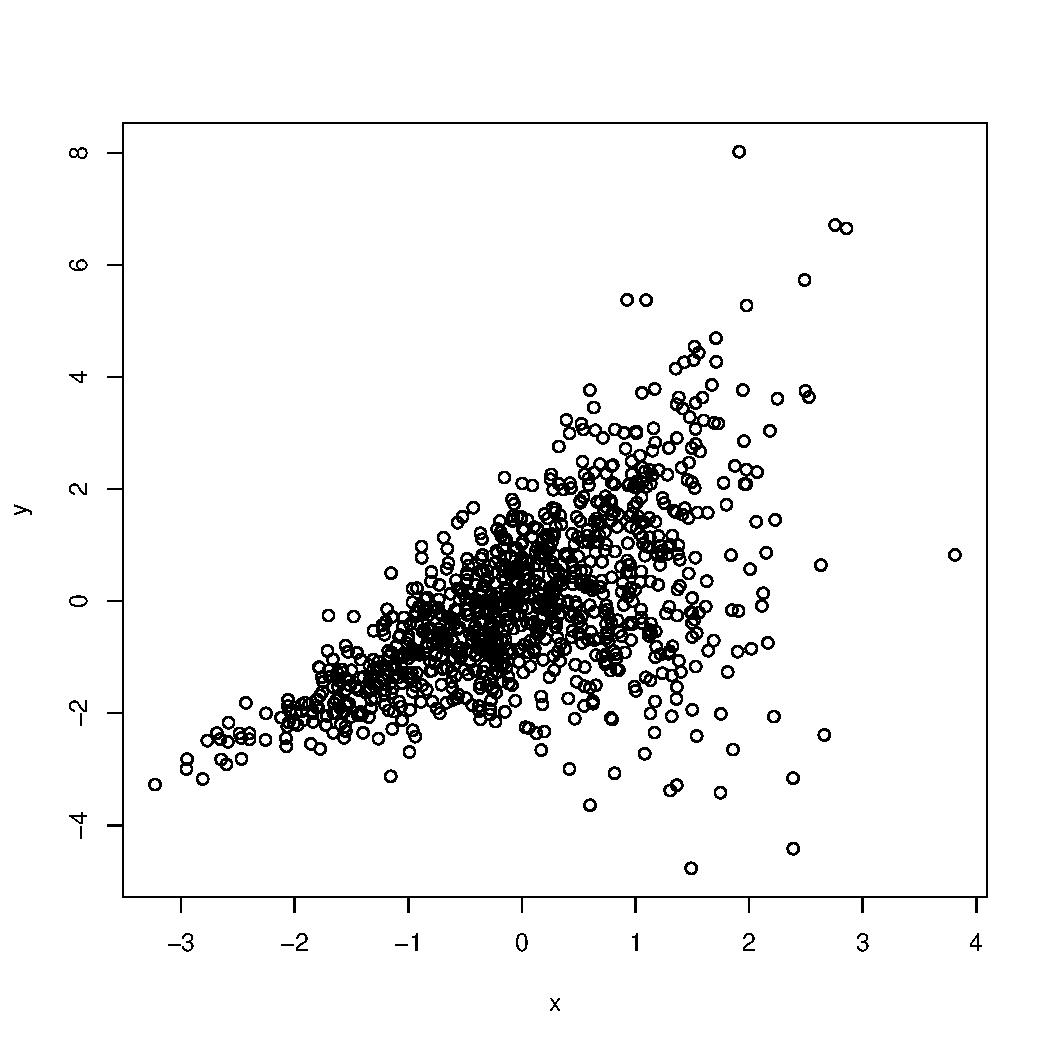
\includegraphics[width=.9\linewidth]{./figures/fig-hetero.pdf}
\end{center}

\subsection{Generate survival time under non proportional hazard (non-PH)}
\label{sec:org3a9eece}

Model:
\lstset{language=r,label= ,caption= ,captionpos=b,numbers=none}
\begin{lstlisting}
mSim <- lvm()
regression(mSim) <- eventtime ~ Gender + Age
regression(mSim) <- s ~ exp(0.6 * Treatment - 0.5 * Gender)
distribution(mSim,~ Treatment + Gender) <- binomial.lvm()
distribution(mSim,~cens) <- coxWeibull.lvm(scale = 1)
distribution(mSim,~eventtime) <- coxWeibull.lvm(scale = 0.3,shape =~ s)
eventTime(mSim) <- time ~ min(eventtime = 1, cens = 0)
\end{lstlisting}

Simulation:
\lstset{language=r,label= ,caption= ,captionpos=b,numbers=none}
\begin{lstlisting}
set.seed(10)
n <- 1e3
df.tempo <- sim(mSim, n = n)
\end{lstlisting}

Display:
\begin{center}
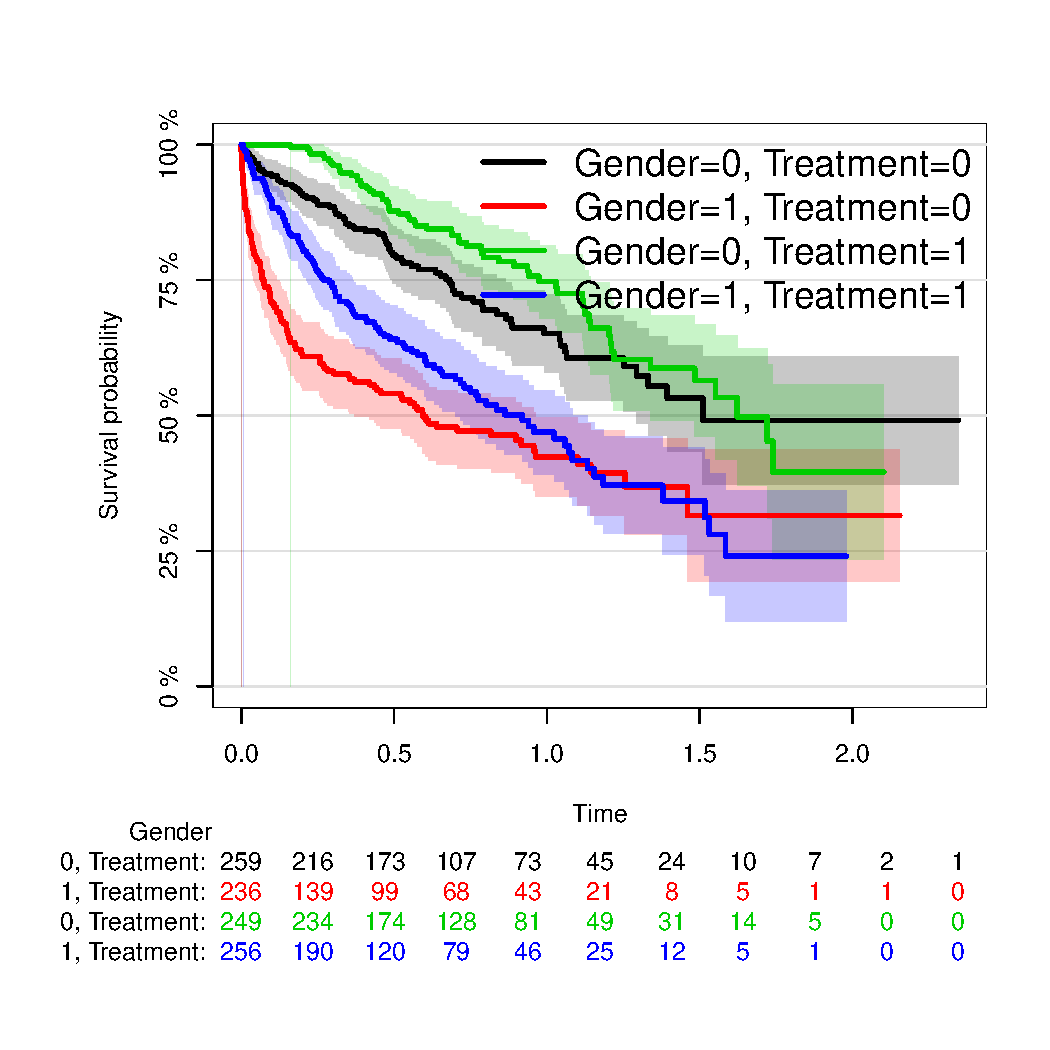
\includegraphics[width=.9\linewidth]{./figures/fig-nonPH.pdf}
\end{center}

\subsection{Generate survival time with delayed treatment effect}
\label{sec:orgb7d5132}

Generative model with non-PH group effect but no Age effect:
\lstset{language=r,label= ,caption= ,captionpos=b,numbers=none}
\begin{lstlisting}
rates1 <- c(0.25,0.5,0.1); cuts <- c(0,3,5)
rates2 <- c(0.25,0.1,0.1); cuts <- c(0,3,5)
lasttime <- 20

m1 <- lvm(Age[50:5]~1)
m2 <- lvm(Age[50:5]~1)
distribution(m1,~eventtime) <- coxExponential.lvm(rate=rates1,timecut=cuts)
distribution(m2,~eventtime) <- coxExponential.lvm(rate=rates2,timecut=cuts)
transform(m1,status~eventtime) <- function(x){as.numeric(x[,1]<= lasttime)}
transform(m2,status~eventtime) <- function(x){as.numeric(x[,1]<= lasttime)}
transform(m1,time~eventtime) <- function(x){pmin(lasttime,x[,1])}
transform(m2,time~eventtime) <- function(x){pmin(lasttime,x[,1])}
latent(m1) <- ~eventtime
latent(m2) <- ~eventtime
\end{lstlisting}

Simulate data:
\lstset{language=r,label= ,caption= ,captionpos=b,numbers=none}
\begin{lstlisting}
set.seed(12)
n <- 500
d1 <- as.data.table(sim(m1,n,latent=FALSE))
d2 <- as.data.table(sim(m2,n,latent=FALSE))
dt.data <- rbind(cbind(d1,group="treatment"),cbind(d2,group="placebo"))
dt.data
\end{lstlisting}

\begin{verbatim}
           Age status       time     group
   1: 46.68935      1  3.8755119 treatment
   2: 53.52666      1  3.2816799 treatment
   3: 47.86065      1  0.8515517 treatment
   4: 47.94281      1 10.1313180 treatment
   5: 45.53314      1  2.6198951 treatment
  ---                                     
 996: 46.47948      1  2.1560011   placebo
 997: 52.78256      1  6.6831242   placebo
 998: 45.10627      1  6.0589065   placebo
 999: 49.24545      1 12.5248064   placebo
1000: 49.08839      1  1.9096902   placebo
\end{verbatim}

Display survival curves by group:
\begin{center}
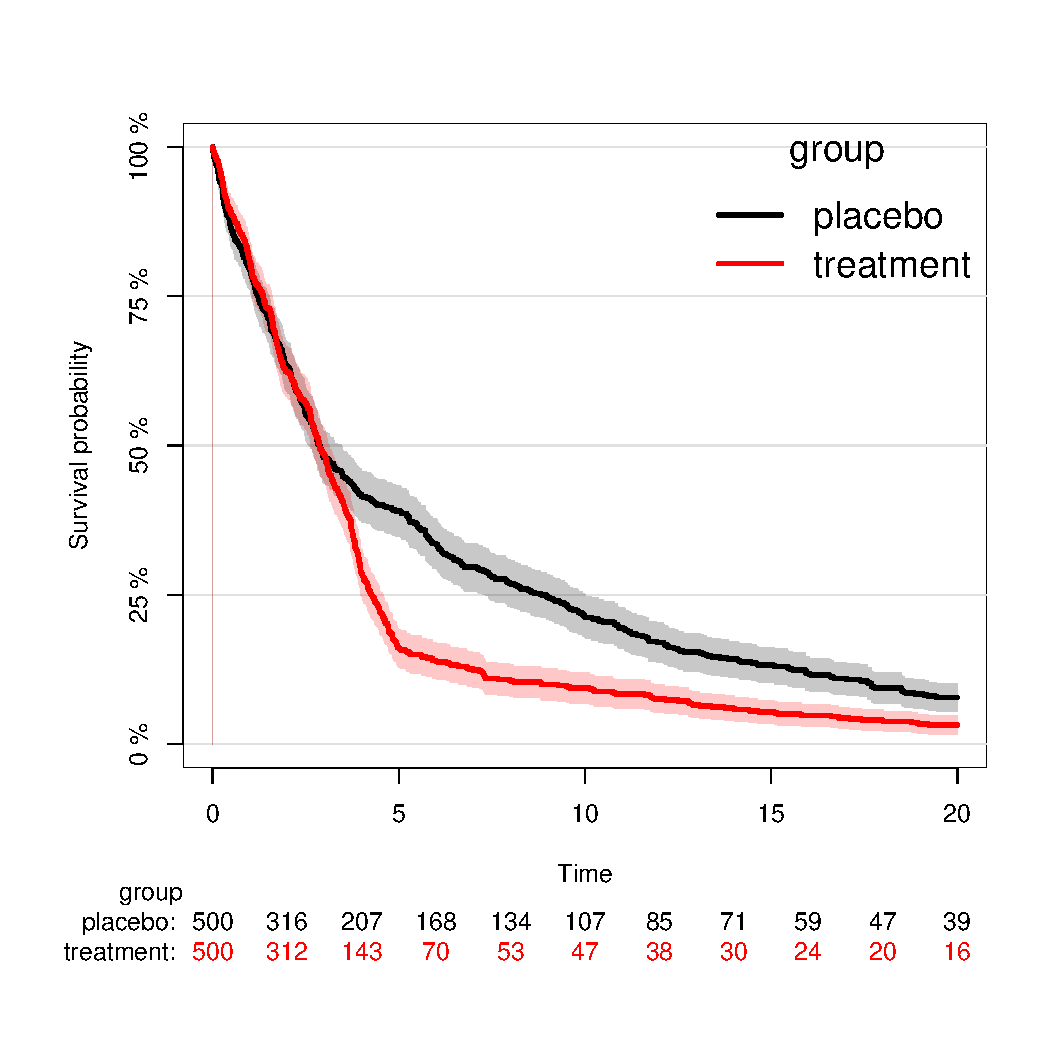
\includegraphics[width=.9\linewidth]{./figures/fig-delayedTreatmentEffect.pdf}
\end{center}

\subsection{Tune optimization parameters}
\label{sec:org5e5a55f}
\subsection{Interaction in lava (mean coefficients)}
\label{sec:orgdf5955a}

\lstset{language=r,label= ,caption= ,captionpos=b,numbers=none}
\begin{lstlisting}
library(lava)
set.seed(10)
data(mtcars, package = "datasets")
mtcars$vs <- as.factor(mtcars$vs)

e.lmI <- lm(mpg ~ vs*drat, data = mtcars)
coef(e.lmI)

e.lmI.bis <- lm(mpg ~ vs + drat:vs, data = mtcars)
coef(e.lmI.bis)
\end{lstlisting}

\begin{verbatim}
(Intercept)         vs1        drat    vs1:drat 
 -0.2127763   1.6821904   4.9611853   1.0211986
(Intercept)         vs1    vs0:drat    vs1:drat 
 -0.2127763   1.6821904   4.9611853   5.9823839
\end{verbatim}


With lava using a single latent variable model (LVM):
\lstset{language=r,label= ,caption= ,captionpos=b,numbers=none}
\begin{lstlisting}
mtcars$vs0drat <- (mtcars$vs=="0")*mtcars$drat
mtcars$vs1drat <- (mtcars$vs=="1")*mtcars$drat

e.lvm <- estimate(lvm(mpg ~ vs + vs0drat+ vs1drat), data = mtcars)
coef(e.lvm)
estimate(e.lvm, function(p){
  p["mpg~vs1drat"] - p["mpg~vs0drat"]
})
\end{lstlisting}

\begin{verbatim}
        mpg mpg~vs0drat mpg~vs1drat     mpg~vs1    mpg~~mpg 
 -0.2127763   4.9611853   5.9823839   1.6821904  13.0157822
            Estimate Std.Err  2.5% 97.5% P-value
mpg~vs1drat    1.021   2.169 -3.23 5.272  0.6378
\end{verbatim}


An alternative implementation uses two LVMs, one per group and where
the variance coefficients are constrain to be the same between groups:
\lstset{language=r,label= ,caption= ,captionpos=b,numbers=none}
\begin{lstlisting}
e2.lvm <- estimate(list(lvm(mpg[mu0:sigma] ~ beta0*drat),
                        lvm(mpg[mu1:sigma] ~ beta1*drat)),
                   data = split(mtcars,mtcars$vs))
coef(e2.lvm)
\end{lstlisting}

\begin{verbatim}
     mpg@1      mpg@2 mpg~drat@1 mpg~~mpg@1 mpg~drat@2 
-0.2127763  1.4694141  4.9611853 13.0157822  5.9823839
\end{verbatim}


Note that \texttt{stats::lm} and \texttt{lava::estimate} should return the same
point estimate but will not quantify the uncertainty similarly. The
standard error \texttt{stats::lm} is more precise as it uses restricted
maximum likelihood (REML) instead of maximum likelihood
(ML). \texttt{stats::lm} also uses a Student's t-distribution instead of a
Gaussian distribution which provides better type 1 error control in
finite samples. 

\subsection{Output correlation between two endogenous variables}
\label{sec:org16c2fb1}
Simulate some data:
\lstset{language=r,label= ,caption= ,captionpos=b,numbers=none}
\begin{lstlisting}
library(lava)
mSim <-lvm(c(gene1,gene2,gene3,gene4,gene5)~expression,
           expression~score)
covariance(mSim) <- gene2 ~ gene3
latent(mSim) <- ~expression

set.seed(10)
d <- lava::sim(mSim, n = 400, latent = FALSE)
\end{lstlisting}

Fit the lvm:
\lstset{language=r,label= ,caption= ,captionpos=b,numbers=none}
\begin{lstlisting}
m <- mSim
e <- lava::estimate(m, data = d)
\end{lstlisting}
Estimate correlation via \emph{lava}:
\lstset{language=r,label= ,caption= ,captionpos=b,numbers=none}
\begin{lstlisting}
cov2cor(attr(predict(e),"cond.var"))
\end{lstlisting}

\begin{verbatim}
          gene1     gene2     gene3     gene4     gene5
gene1 1.0000000 0.5236249 0.5204666 0.4945280 0.5354561
gene2 0.5236249 1.0000000 0.7623392 0.4711268 0.5101182
gene3 0.5204666 0.7623392 1.0000000 0.4682851 0.5070414
gene4 0.4945280 0.4711268 0.4682851 1.0000000 0.4817718
gene5 0.5354561 0.5101182 0.5070414 0.4817718 1.0000000
\end{verbatim}


Estimate correlation via \texttt{lvmCov2Cor} (only correlation through the latent variable):
\lstset{language=r,label= ,caption= ,captionpos=b,numbers=none}
\begin{lstlisting}
lvmCov2Cor(e, var1 = "gene1", var2 = "gene2")
\end{lstlisting}

\begin{verbatim}
                        variable  estimate         se     lower     upper null p.value
variance 1                 gene1 2.0942854 0.13667200 1.8264133 2.3621576   NA      NA
variance 2                 gene2 2.2976185 0.14862591 2.0063171 2.5889200   NA      NA
direct covariance  (gene1,gene2) 0.0000000 0.00000000 0.0000000 0.0000000    0     NaN
total covariance   (gene1,gene2) 1.1486221 0.10851604 0.9359345 1.3613096    0       0
direct correlation (gene1,gene2) 0.0000000 0.00000000 0.0000000 0.0000000    0     NaN
total correlation  (gene1,gene2) 0.5236249 0.03010923 0.4646119 0.5826379    0       0
\end{verbatim}


Estimate correlation via \texttt{lvmCov2Cor} (direct and indirect correlation):
\lstset{language=r,label= ,caption= ,captionpos=b,numbers=none}
\begin{lstlisting}
lvmCov2Cor(e, var1 = "gene2", var2 = "gene3")
\end{lstlisting}

\begin{verbatim}
                        variable  estimate         se     lower     upper null      p.value
variance 1                 gene2 2.2976185 0.14862591 2.0063171 2.5889200   NA           NA
variance 2                 gene3 1.9920357 0.12875100 1.7396884 2.2443830   NA           NA
direct covariance  (gene2,gene3) 0.5701469 0.08197808 0.4094728 0.7308210    0 3.528955e-12
total covariance   (gene2,gene3) 1.6309317 0.12469211 1.3865396 1.8753237    0 0.000000e+00
direct correlation (gene2,gene3) 0.2665012 0.03458231 0.1987212 0.3342813    0 1.287859e-14
total correlation  (gene2,gene3) 0.7623392 0.02017803 0.7227910 0.8018874    0 0.000000e+00
\end{verbatim}


Estimate the correlation via \emph{lava} (manual version):
\lstset{language=r,label= ,caption= ,captionpos=b,numbers=none}
\begin{lstlisting}
estimate(e, function(x){
  var.gene1 <- x["gene1~~gene1"] + x["expression~~expression"]
  var.gene2 <- x["gene2~~gene2"] + x["gene2~expression"]^2 * x["expression~~expression"]
  cov.gene12 <- x["gene2~expression"] * x["expression~~expression"]
  c(var.gene1 = var.gene1,
    var.gene2 = var.gene2,
    cov = cov.gene12,
    cor = cov.gene12/sqrt(var.gene1 * var.gene2))
})
\end{lstlisting}

\begin{verbatim}
                       Estimate Std.Err   2.5%  97.5%   P-value
var.gene1.gene1~~gene1   2.0943 0.13327 1.8331 2.3555 1.191e-55
var.gene2.gene2~~gene2   2.2976 0.14104 2.0212 2.5741 1.163e-59
cov.gene2~expression     1.1486 0.10913 0.9347 1.3625 6.600e-26
cor.gene2~expression     0.5236 0.03115 0.4626 0.5847 2.024e-63
\end{verbatim}

\subsection{Output correlation between two latent variables}
\label{sec:org1122d7a}

Simulate some data:
\lstset{language=r,label= ,caption= ,captionpos=b,numbers=none}
\begin{lstlisting}
library(lava)
mSim <-lvm(c(PEQ_poslife,PEQ_posself,PEQ_posmood,PEQ_possoc,PEQ_posbehav)~lv.peq,
           c(MEQ_mystical,MEQ_mood) ~ 1*lv.meq,
           c(MEQ_timespace,MEQ_ineffability) ~ lv.meq,
           lv.meq[0:2]~1,
           lv.peq[0:0.25]~1)
covariance(mSim) <- lv.peq ~ lv.meq
covariance(mSim) <- MEQ_timespace~MEQ_ineffability
latent(mSim) <- ~lv.peq+lv.meq

set.seed(10)
d <- sim(mSim, n = 40, latent = FALSE)
\end{lstlisting}

Fit the lvm:
\lstset{language=r,label= ,caption= ,captionpos=b,numbers=none}
\begin{lstlisting}
m1 <-lvm(c(PEQ_poslife,PEQ_posself,PEQ_posmood,PEQ_possoc,PEQ_posbehav)~lv.peq,
         c(MEQ_mystical,MEQ_mood) ~ 1*lv.meq,
         c(MEQ_timespace,MEQ_ineffability) ~ lv.meq)
covariance(m1) <- lv.peq ~ lv.meq
covariance(m1) <- MEQ_timespace~MEQ_ineffability
latent(m1) <- ~lv.peq
latent(m1) <- ~lv.meq
e <- estimate(m1, d)
\end{lstlisting}

Estimate the correlation via \emph{lava}:
\lstset{language=r,label= ,caption= ,captionpos=b,numbers=none}
\begin{lstlisting}
estimate(e, function(x){
    c(var.meq = x["lv.meq~~lv.meq"],
      var.peq = x["lv.peq~~lv.peq"],
      cov = x["lv.peq~~lv.meq"],
      cor = x["lv.peq~~lv.meq"]/sqrt(x["lv.peq~~lv.peq"]*x["lv.meq~~lv.meq"]))
})
\end{lstlisting}

\begin{verbatim}
                       Estimate Std.Err     2.5%  97.5%   P-value
var.meq.lv.meq~~lv.meq   2.4150  0.6270  1.18606 3.6439 0.0001174
var.peq.lv.peq~~lv.peq   0.1808  0.1133 -0.04126 0.4030 0.1105233
cov.lv.peq~~lv.meq       0.4022  0.1885  0.03268 0.7717 0.0329009
cor.lv.peq~~lv.meq       0.6086  0.1638  0.28748 0.9296 0.0002034
\end{verbatim}


Estimate the correlation via \texttt{lvmCov2Cor}:
\lstset{language=r,label= ,caption= ,captionpos=b,numbers=none}
\begin{lstlisting}
lvmCov2Cor(e, var1 = "lv.meq", var2 = "lv.peq", robust = TRUE)
\end{lstlisting}

\begin{verbatim}
                          variable  estimate        se       lower     upper
variance 1                  lv.meq 2.4149694 0.6270062  1.18605985 3.6438789
variance 2                  lv.peq 0.1808441 0.1133218 -0.04126259 0.4029509
direct covariance  (lv.meq,lv.peq) 0.4021716 0.1885216  0.03267591 0.7716672
total covariance   (lv.meq,lv.peq) 0.4021716 0.1885216  0.03267591 0.7716672
direct correlation (lv.meq,lv.peq) 0.6085599 0.1638215  0.28747555 0.9296442
total correlation  (lv.meq,lv.peq) 0.6085599 0.1638215  0.28747555 0.9296442
                   null     p.value
variance 1           NA          NA
variance 2           NA          NA
direct covariance     0 0.032900854
total covariance      0 0.032900854
direct correlation    0 0.000203386
total correlation     0 0.000203386
\end{verbatim}

\subsection{Handling left, right, and interval censored data}
\label{sec:org17abbb0}

Simulate data:
\lstset{language=r,label= ,caption= ,captionpos=b,numbers=none}
\begin{lstlisting}
n <- 10000
tau <- c(left = -2, right = 2)

set.seed(10)
X <- rnorm(n)
Y <- rnorm(n, mean = X)
df <- data.frame(Y=Y,X=X)
\end{lstlisting}

Right censoring:
\lstset{language=r,label= ,caption= ,captionpos=b,numbers=none}
\begin{lstlisting}
df$YobsR <- pmin(Y,tau["right"])
df$censR <- Y>tau["right"]

df$SurvR <- Surv(df$YobsR,df$censR==FALSE, type = "right")

rbind(naive = coef(lm(YobsR ~ X, data = df)),
      corrected = coef(estimate(lvm(SurvR ~ X), df))[1:2])
\end{lstlisting}

\begin{verbatim}
          (Intercept)         X
naive     -0.07039338 0.9290829
corrected -0.02081243 1.0065446
\end{verbatim}


Left censoring:
\lstset{language=r,label= ,caption= ,captionpos=b,numbers=none}
\begin{lstlisting}
df$YobsL <- pmax(Y,tau["left"])
df$censL <- Y< (tau["left"])

df$SurvL <- Surv(df$YobsL,df$censL==FALSE, type = "left")

rbind(naive = coef(lm(YobsL ~ X, data = df)),
      corrected = coef(estimate(lvm(SurvL ~ X), df))[1:2])
\end{lstlisting}

\begin{verbatim}
          (Intercept)         X
naive      0.03314233 0.9150299
corrected -0.02171591 0.9991420
\end{verbatim}


Interval censoring:
\lstset{language=r,label= ,caption= ,captionpos=b,numbers=none}
\begin{lstlisting}
df$Yobs <- pmax(pmin(Y,tau["right"]),tau["left"])
df$Surv <- Surv(time = ifelse(df$censL,-Inf,df$YobsR),
                time2 = ifelse(df$censR,+Inf,df$YobsL),
                type = "interval2")

rbind(naive = coef(lm(Yobs ~ X, data = df)),
      corrected = coef(estimate(lvm(Surv ~ X), df))[1:2]) ## FAILS
\end{lstlisting}

\subsection{LVM as a weighted mean}
\label{sec:org6107d64}
Simulate some data:
\lstset{language=r,label= ,caption= ,captionpos=b,numbers=none}
\begin{lstlisting}
library(lava)

mSim <- lvm(coldPain ~ 0.1*age + 1*etaPain,
            heatPain ~ 0.1*age + 2*etaPain,
            musclePain ~ 0.1*age + 0.5*etaPain,
            tolerancePain ~ 0.1*age + 2*etaPain,
            etaPain ~ status)
latent(mSim) <- ~etaPain
distribution(mSim, ~status) <- binomial.lvm()
## distribution(mSim, ~coldPain+heatPain+musclePain+tolerantcePain) <- Gamma.lvm(rate = 2, shape = 10)
distribution(mSim, ~age) <- gaussian.lvm(mean = 30, sd = 5)

set.seed(10)
d <- sim(mSim, 1e3, latent = FALSE)
\end{lstlisting}

Estimate LVM with constraints on the latent variable:
\lstset{language=r,label= ,caption= ,captionpos=b,numbers=none}
\begin{lstlisting}
m <- lvm(coldPain ~ age + etaPain,
         heatPain ~ age + etaPain,
         musclePain ~ age + etaPain,
         tolerancePain ~ age + etaPain,
         etaPain ~ status)
latent(m) <- ~etaPain
e <- estimate(m, data = d)
\end{lstlisting}

Extract fitted latent variable values:
\lstset{language=r,label= ,caption= ,captionpos=b,numbers=none}
\begin{lstlisting}
LV.predict <- predict(e, x = manifest(e), y = latent(e))
c(tapply(LV.predict,d$status,mean), coef(e)["etaPain~status"])
\end{lstlisting}

\begin{verbatim}
         0              1 etaPain~status 
0.01286411     0.92152131     0.90865707
\end{verbatim}


\clearpage

Manually compute weights: 
\lstset{language=r,label= ,caption= ,captionpos=b,numbers=none}
\begin{lstlisting}
## residuals
epsilon <- residuals(e) 
## all coef
e.allCoef <- summary(e)$coef[,"Estimate"]
## variance-covariance matrices matrices
lambda <- e.allCoef[paste0(endogenous(e),"~",latent(e))]
mu <- e.allCoef[endogenous(e)]
tau <- e.allCoef[paste0(latent(e),"~~",latent(e))]
sigma <- e.allCoef[paste0(endogenous(e),"~~",endogenous(e))]

Sigma22 <- tcrossprod(lambda)*tau + diag(sigma)
Sigma12 <- rbind(lambda*tau)
weight <- Sigma12 %*% solve(Sigma22)
weight
\end{lstlisting}

\begin{verbatim}
          [,1]      [,2]       [,3]      [,4]
[1,] 0.1108541 0.2186568 0.04547272 0.1854233
\end{verbatim}


and values of the latent variable:
\lstset{language=r,label= ,caption= ,captionpos=b,numbers=none}
\begin{lstlisting}
nu <- e.allCoef[latent(e)]
Gamma <- as.double(e.allCoef[paste0(latent(e),"~status")] %*% d$status)

LV.manual <- nu + Gamma + as.double(weight %*% t(epsilon))
range(LV.manual - LV.predict)
\end{lstlisting}

\begin{verbatim}
[1] -1.332268e-15  6.217249e-15
\end{verbatim}

\subsection{Standardized coefficients}
\label{sec:org9e6dbed}

"The standardized coefficients in the last column are interpreted as
the change in standard deviation of the outcome when increasing the
predictor one standard deviation" (Holst 2013).

\bigskip

Simulate some data:
\lstset{language=r,label= ,caption= ,captionpos=b,numbers=none}
\begin{lstlisting}
library(data.table);library(lava)
mSim <- lvm(Y1~X+1*eta,Y2~X+2*eta,Y3~X+3*eta)
latent(mSim) <- ~eta
n <- 2500
set.seed(10)
d <- sim(mSim, n=n, latent = FALSE)
\end{lstlisting}

Linear regression:
\lstset{language=r,label= ,caption= ,captionpos=b,numbers=none}
\begin{lstlisting}
## by hand
e <- estimate(lvm(Y1~Y2+Y3), data = d)
coef(e)["Y1~Y2"]*sd(d$Y2)/sd(d$Y1)
## via the dataset
eS <- estimate(lvm(Y1~Y2+Y3), data = scale(d))
as.data.frame(coef(eS, std = "xy", type = 9))[1,,drop=FALSE]
\end{lstlisting}

\begin{verbatim}
    Y1~Y2 
0.4167574
       Estimate Std. Error  Z-value     P-value    std.xy
Y1~Y2 0.4167574 0.02738807 15.21675 2.73795e-52 0.4167574
\end{verbatim}


LVM with saturated variance model:
\lstset{language=r,label= ,caption= ,captionpos=b,numbers=none}
\begin{lstlisting}
m <- lvm(Y1~X+eta,Y2~X+eta,Y3~X+eta)
latent(m) <- ~eta

## by hand
e <- estimate(m, data = d)
coef(e)["Y1~X"]*sd(d$X)/sd(d$Y1)

## via the dataset
eS <- estimate(m, data = scale(d))
as.data.frame(coef(eS, std = "xy", type = 9))[1,,drop=FALSE]

## in that case the marginal variance equals the modelled one
c(model=coef(e)["Y1~~Y1"]+coef(e)["eta~~eta"]+var(d$X)*coef(e)["Y1~X"]^2,
  marginal=var(d$Y1))
## minor difference due to /(n-1) instead of /n in var
\end{lstlisting}

\begin{verbatim}
     Y1~X 
0.5858683
      Estimate Std. Error  Z-value       P-value    std.xy
Y1~X 0.5858683 0.01620812 36.14658 4.209965e-286 0.5858683
model.Y1~~Y1     marginal 
    3.033911     3.034709
\end{verbatim}


Non-saturated LVM:
\lstset{language=r,label= ,caption= ,captionpos=b,numbers=none}
\begin{lstlisting}
m <- lvm(Y1~X+1*eta,Y2~X+1*eta,Y3~X+1*eta)
latent(m) <- ~eta

## by hand
e <- estimate(m, data = d)
coef(e)["Y1~X"]*sd(d$X)/sd(d$Y1)
coef(e)["Y1~X"]*sd(d$X)/sqrt(coef(e)["Y1~~Y1"]+coef(e)["eta~~eta"]+var(d$X)*coef(e)["Y1~X"]^2)
as.data.frame(coef(e, std = "xy", type = 9))[1,,drop=FALSE]

## real difference between modeled and marginal variance
c(model=coef(e)["Y1~~Y1"]+coef(e)["eta~~eta"]+var(d$X)*coef(e)["Y1~X"]^2,
  marginal=var(d$Y1))
\end{lstlisting}

\begin{verbatim}
     Y1~X 
0.5858683
     Y1~X 
0.5645535
      Estimate Std. Error  Z-value       P-value    std.xy
Y1~X 0.9977775 0.02918153 34.19209 3.169765e-256 0.5644766
model.Y1~~Y1     marginal 
    3.268187     3.034709
\end{verbatim}


After re-scaling the data, not sure what the \texttt{std.xy}:
\lstset{language=r,label= ,caption= ,captionpos=b,numbers=none}
\begin{lstlisting}
eS <- estimate(m, data = scale(d))
as.data.frame(coef(eS, std = "xy", type = 9))[1,,drop=FALSE]
\end{lstlisting}

\begin{verbatim}
      Estimate Std. Error  Z-value       P-value    std.xy
Y1~X 0.5858683 0.02003958 29.23556 6.852072e-188 0.5047583
\end{verbatim}


is though.

\section{Miscellaneous}
\label{sec:orgc698778}
\subsection{Profile code R}
\label{sec:org18d6aa9}

\lstset{language=r,label= ,caption= ,captionpos=b,numbers=none}
\begin{lstlisting}
library(lava)
m <- lvm(Y ~ X + G)
FUN <- function(n){
    d <- lava::sim(m, n = n)
    estimate(m,d)
}
\end{lstlisting}

\#+RESULTS[\textit{<2019-06-27 to 09:37> } a0d5077301cabedce939985d9ce7fb7eb9072578]:

\lstset{language=r,label= ,caption= ,captionpos=b,numbers=none}
\begin{lstlisting}
profvis::profvis(FUN(n = 500))
profvis::profvis(FUN(n = 5000))
profvis::profvis(FUN(n = 50000))
\end{lstlisting}

\begin{verbatim}
[1] 14.9 16.4 31.4 81.2
\end{verbatim}


\lstset{language=r,label= ,caption= ,captionpos=b,numbers=none}
\begin{lstlisting}
Rprof(tf <- "rprof.log", memory.profiling=TRUE)
xx <- FUN(n=500000)
Rprof(NULL)
max(summaryRprof(tf, memory = "both")$by.total$mem.total)

\end{lstlisting}

\begin{verbatim}
[1] 129.8
\end{verbatim}

\subsection{Profile code C}
\label{sec:org6bfbe11}
R -d "valgrind --tool=cachegrind" -f myfile.R
R -d "valgrind --tool=callgrind" -f myfile.R
\url{https://kcachegrind.github.io/html/Home.html}

\subsection{Debug}
\label{sec:org42fa067}
To not show to many line before debug:
\lstset{language=r,label= ,caption= ,captionpos=b,numbers=none}
\begin{lstlisting}
options(deparse.max.lines = 200)
\end{lstlisting}

To show at which line in the program an error occured:
\lstset{language=r,label= ,caption= ,captionpos=b,numbers=none}
\begin{lstlisting}
options(error = function()revTraceback(max.lines = 5))
\end{lstlisting}

\subsection{Find all function names from a package}
\label{sec:org7d5b5c0}
\lstset{language=r,label= ,caption= ,captionpos=b,numbers=none}
\begin{lstlisting}
r <- unclass(lsf.str(envir = asNamespace("lava"), all = T))
r[grep("coef", r)]
\end{lstlisting}

\begin{verbatim}
 [1] "coef.CrossValidated"   "coef.effects"          "coef.estimate"         "coef.estimate.list"   
 [5] "coef.lvm"              "coef.lvm.mixture"      "coef.lvmfit"           "coef.multigroup"      
 [9] "coef.multigroupfit"    "coef.multinomial"      "coef.ordreg"           "coef.pcor"            
[13] "coef.summary.estimate" "coef.summary.lvmfit"   "coef.twostageCV"       "coef.zibreg"          
[17] "describecoef"          "excoef"                "stdcoef"
\end{verbatim}

\subsection{Install development version of R}
\label{sec:org753085a}
\url{https://cran.r-project.org/bin/windows/base/rdevel.html}

\subsection{Install suggested packages}
\label{sec:org6cf2cdf}

\lstset{language=r,label= ,caption= ,captionpos=b,numbers=none}
\begin{lstlisting}
char.package <- utils::packageDescription("butils", fields = "Suggests")
vec.package <- unlist(strsplit(gsub("[[:blank:]]", "", charPackage), split = ","))
install.packages(vec.package)
\end{lstlisting}

\subsection{R version}
\label{sec:org6cd2f26}

\lstset{language=r,label= ,caption= ,captionpos=b,numbers=none}
\begin{lstlisting}
sessionInfo()
\end{lstlisting}

\begin{verbatim}
R version 3.5.1 (2018-07-02)
Platform: x86_64-w64-mingw32/x64 (64-bit)
Running under: Windows 7 x64 (build 7601) Service Pack 1

Matrix products: default

locale:
[1] LC_COLLATE=Danish_Denmark.1252  LC_CTYPE=Danish_Denmark.1252    LC_MONETARY=Danish_Denmark.1252
[4] LC_NUMERIC=C                    LC_TIME=Danish_Denmark.1252    

attached base packages:
[1] parallel  stats     graphics  grDevices utils     datasets  methods   base     

other attached packages:
 [1] ggpubr_0.2         magrittr_1.5       officer_0.3.2      Publish_2018.04.17 lava_1.6.5        
 [6] doSNOW_1.0.16      snow_0.4-3         iterators_1.0.10   foreach_1.4.4      pbapply_1.3-4     
[11] multcomp_1.4-8     TH.data_1.0-9      MASS_7.3-50        mvtnorm_1.0-8      survival_2.44-1.1 
[16] prodlim_2018.04.18 car_3.0-2          carData_3.0-2      ggplot2_3.1.0      data.table_1.12.0 

loaded via a namespace (and not attached):
 [1] Rcpp_1.0.1        lattice_0.20-35   visNetwork_2.0.4  zoo_1.8-4         assertthat_0.2.0 
 [6] digest_0.6.17     R6_2.3.0          cellranger_1.1.0  plyr_1.8.4        pillar_1.3.1     
[11] rlang_0.3.1       lazyeval_0.2.1    curl_3.2          readxl_1.1.0      uuid_0.1-2       
[16] Matrix_1.2-14     labeling_0.3      splines_3.5.1     stringr_1.3.1     foreign_0.8-70   
[21] htmlwidgets_1.3   munsell_0.5.0     compiler_3.5.1    pkgconfig_2.0.2   base64enc_0.1-3  
[26] htmltools_0.3.6   tidyselect_0.2.5  gridExtra_2.3     tibble_2.0.1      rio_0.5.10       
[31] codetools_0.2-15  viridisLite_0.3.0 crayon_1.3.4      dplyr_0.7.8       withr_2.1.2      
[36] grid_3.5.1        jsonlite_1.5      gtable_0.2.0      scales_1.0.0      zip_1.0.0        
[41] stringi_1.2.4     ggthemes_4.0.1    bindrcpp_0.2.2    xml2_1.2.0        sandwich_2.5-0   
[46] cowplot_0.9.3     openxlsx_4.1.0    tools_3.5.1       forcats_0.3.0     glue_1.3.0       
[51] purrr_0.3.0       hms_0.4.2         yaml_2.2.0        abind_1.4-5       colorspace_1.3-2 
[56] bindr_0.1.1       haven_1.1.2
\end{verbatim}

\subsection{Install a package from a zip file (windows)}
\label{sec:orgff69666}
\lstset{language=r,label= ,caption= ,captionpos=b,numbers=none}
\begin{lstlisting}
install.packages("package_version.zip", repos = NULL, type = "win.binary")
\end{lstlisting}
\subsection{Install and load two version of the same package}
\label{sec:orgc499782}

Install
\lstset{language=r,label= ,caption= ,captionpos=b,numbers=none}
\begin{lstlisting}
devtools::install_github("bozenne/BuyseTest") ## v1
install.packages("http://cran.r-project.org/src/contrib/Archive/BuyseTest/BuyseTest_1.0.tar.gz", 
                 lib = "C:/Users/hpl802/Downloads/LIBRTEMPO", type = "source", repos = NULL)
\end{lstlisting}

Load 
\lstset{language=r,label= ,caption= ,captionpos=b,numbers=none}
\begin{lstlisting}
library(BuyseTest) ## v1
detach("package:BuyseTest", unload = TRUE)
library(BuyseTest, lib.loc="C:/Users/hpl802/Downloads/LIBRTEMPO") ## v2
detach("package:BuyseTest", unload = TRUE)
\end{lstlisting}

\subsection{CRAN check rocker}
\label{sec:orgb194454}
\url{https://www.brodieg.com/2018/04/06/adventures-in-r-and-compiled-code/}

docker run --rm -ti -v \$(pwd):/mydir wch1/r-debug
RDvalgrind -e "install.packages('/mydir/fansi\textsubscript{0.2.1.tar.gz}')"
RDvalgrind -d valgrind  \# and run tests

RDcsan

wget -O - \url{https://github.com/bozenne/BuyseTest/tarball/master} | tar xz
\subsection{Regular expressions}
\label{sec:orge3bcf41}
\url{https://posit.co/wp-content/uploads/2022/10/regex.pdf}
\end{document}